%% The "\appendix" call has already been made in the declaration
%% of the "appendices" environment (see thesis.tex).


\chapter{Miscellaneous}
\label{app:noise}
\section{Jet Identification Criteria}
\label{app:jetcriteria}


For Calo jets the following criteria were applied:

\begin{table}[H]
\footnotesize
\begin{center}
\begin{tabulary}{0.80\textwidth}{LL}
\cline{1-2}
\multicolumn{2}{l}{Loose CaloJet Id} \\
Variable & Definition \\ 
\hline\hline
f$_{HPD} < 0.98$ \qquad\qquad\qquad\qquad\qquad\qquad & Fraction of jet energy contributed from ``hottest'' \ac{HPD}, which rejects \ac{HCAL} noise.  \\
f$_{EM} > 0.01$ & Noise from the \ac{HCAL} is further suppressed by requiring a minimal electromagnetic component to the jet f$_{EM}$. \\
N$^{90}_{hits} \geq$ 2 & Jets that have $>$ 90\% of its energy from a single chanel are rejected, to serve as a safety net that catches jets arising from undiagnosed noisy channels.\\
\hline
\end{tabulary}
\end{center}
\caption[Criteria for a reconstructed jet to pass the loose calorimeter jet id.]{Criteria for a reconstructed jet to pass the loose calorimeter jet id.}
\label{tabapp:calojetid}
\end{table}


For PF jets the following criteria were applied:
  
\begin{table}[H]
\footnotesize
\begin{center}
\begin{tabulary}{0.80\textwidth}{p{3.5cm}L}
\cline{1-2}
\multicolumn{2}{l}{Loose PF jet Id} \\
Variable & Definition \\ 
\hline\hline
nfhJet $<$ 0.99 & Fraction of jet composed of neutral hadrons. \ac{HCAL} noise tends to populate high values of neutral 
hadron fraction.\\
nemfJet $<$ 0.99 & Fraction of jet composed of neutral electromagnetic energy. \ac{ECAL} noise tends to populate high values of 
neutral EM fraction. \\
nmultiJet $>$ 1 & Number of constituents that jet is composed from. \\
chfJet $>$ 0 & Fraction of jet composed of charged hadrons. \\
cmultiJet $>$ 0 & Number of charged particles that compose jet. \\
cemfJet $<$ 0.99 & Fraction of jet composed of charged electromagnetic energy. \\
\hline
\end{tabulary}
\end{center}
\caption[Criteria for a reconstructed jet to pass the loose PF jet id.]{Criteria for a reconstructed jet to pass the loose PF jet id.}
\label{apptab:pfjetid}
\end{table}  
  
\section{Primary Vertices}

\label{app:primaryvertices}

The pile-up per event is defined by the number of 'good' reconstructed primary vertices in the event, with each vertex satisfying the following requirements:

\begin{table}[H]
\footnotesize
\begin{center}
\begin{tabulary}{0.80\textwidth}{p{3cm}L}
\cline{1-2}
\multicolumn{2}{l}{Good primary vertex requirement} \\
Variable & Definition \\ 
\hline\hline
$N_{dof} > 4$ \qquad\qquad\qquad & The number of degree of freedom, from the vertex fit to compute the best estimate of the vertex parameters. \\
$\vert \Delta z_{vtx} \vert < 24$cm &  The distance, $\vert\Delta z_{vex}\vert$, to the position of the closest \ac{HLT} primary vertex. \\ 
 $\rho < 2$cm & The perpendicular distance of track position to the beam spot. \\
\cline{1-2}
\end{tabulary}
\end{center}
\caption[Criteria for a vertex in an event to be classified as a 'good' reconstructed primary vertex.]{Criteria for a vertex in an event to be classified as a 'good' reconstructed primary vertex.}
\label{tabapp:primaryvertices}
\end{table}

\chapter{L1 Jets}

\section{Jet Matching Efficiencies}
\label{app:jetmatching}

The single jet turn-on curves are derived from events independent of whether the leading jet in an event is matched to a Level 1 jet using $\Delta R$ matching detailed in Section  (\ref{subsec:l1jettrigeff}) or not.  These turn-ons are produced from events which are not triggered on jet quantities and therefore it is not guaranteed that the lead jet of an event will be seeded by a Level 1 jet. Figure \ref{fig:leadjetmatcheff} shows the particular matching efficiency of a lead jet to a L1 jet.

\begin{figure}[htp]
\centering
\resizebox{.7\linewidth}{0.5\height}{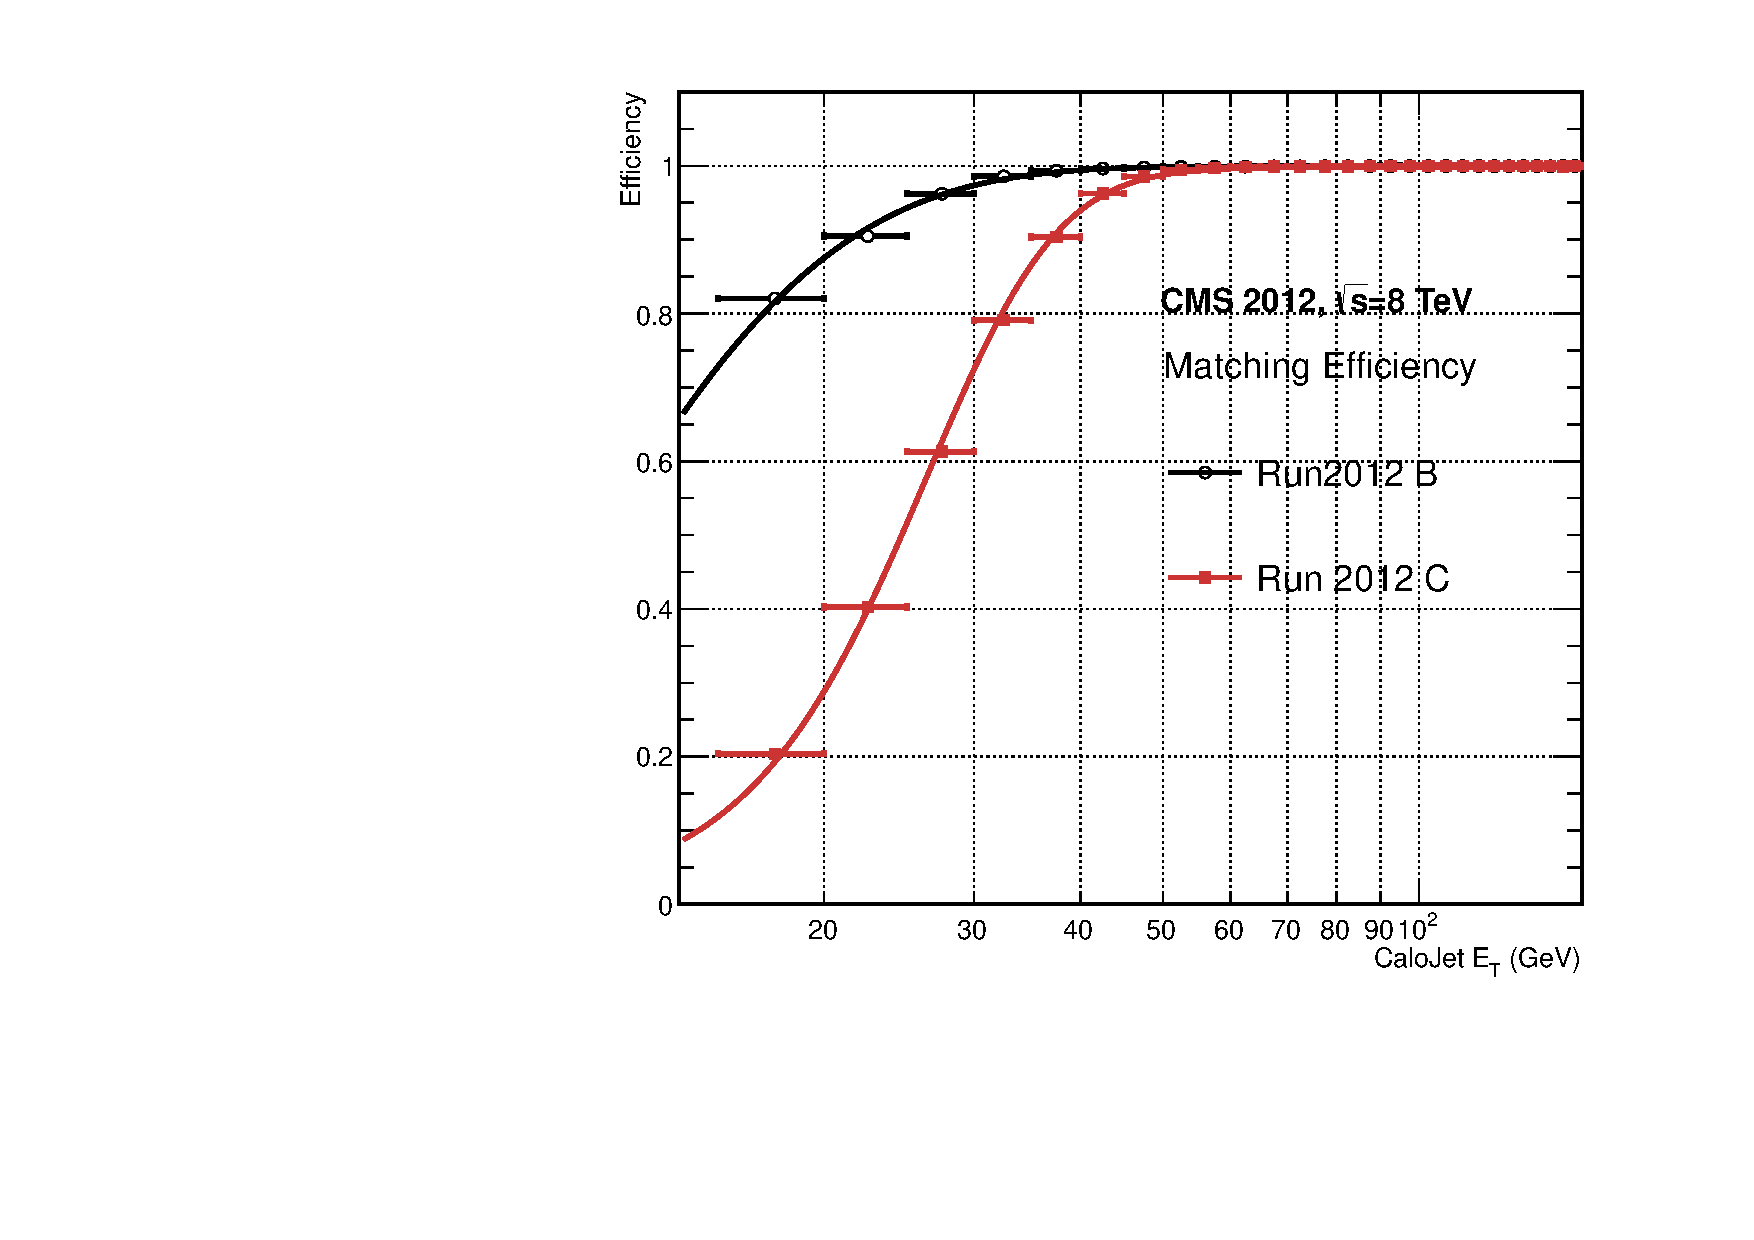
\includegraphics{plots/leadjet_matchingeff.pdf}}
\caption[Leading jet matching efficiency as a function of the offline CaloJet $\et$.]{Leading jet matching efficiency as a function of the offline CaloJet $\et$, measured in an isolated muon triggered dataset in the 2012B and 2012C run periods.}
  \label{fig:leadjetmatcheff}
\end{figure}

It can be seen that the turn on is sharper during the 2012B run period. The seed threshold requirement of a 5 \GeV jet seed in run 2012C results in more events in which even the lead offline jet does not have an associated L1 jet. For larger jet $\et$ thresholds, typical of thresholds used in physics analyses, 100$\%$ efficiency is observed, and therefore this effect has no impact to overall physics performance.

The matching efficiencies have a $\mu$ values of 6.62 GeV and 19.51 GeV for Run 2012B and 2012C respectively and is shown in Table~\ref{tab:matcheff}. 

\begin{table}
\begin{center}
\begin{tabular*}{0.5\textwidth}{ccc}
\cline{1-3}
\multicolumn{1}{c}{Run Period} & $\mu$ & $\sigma$ \\ \hline\hline
2012B & 6.62 $\pm$ 0.01 & 0.79 $\pm$ 0.03  \\ 
2012C & 19.51 $\pm$ 0.03 & 7.14 $\pm$ 0.02 \\ 
\end{tabular*}
\caption[Results of a cumulative EMG function fit to the turn-on
curves for the matching efficiency of the leading jet in an event to
a Level-1 jet in run 2012C and 2012B data.]{Results of a cumulative EMG function fit to the turn-on
curves for the matching efficiency of the leading jet in an event to
a Level-1 jet in run 2012C and 2012B data, measured in an isolated
muon triggered sample. The turn-on point, $\mu$, and resolution, $\sigma$, are measured with respect to offline Calo Jet $\et$.} \label{tab:matcheff}
\end{center}
\end{table}

\section{Leading Jet Energy Resolution}
\label{app:jetpuresolution}

\begin{figure}[ht]
    \centering
    \begin{minipage}[b]{0.98\linewidth}
    \centering
   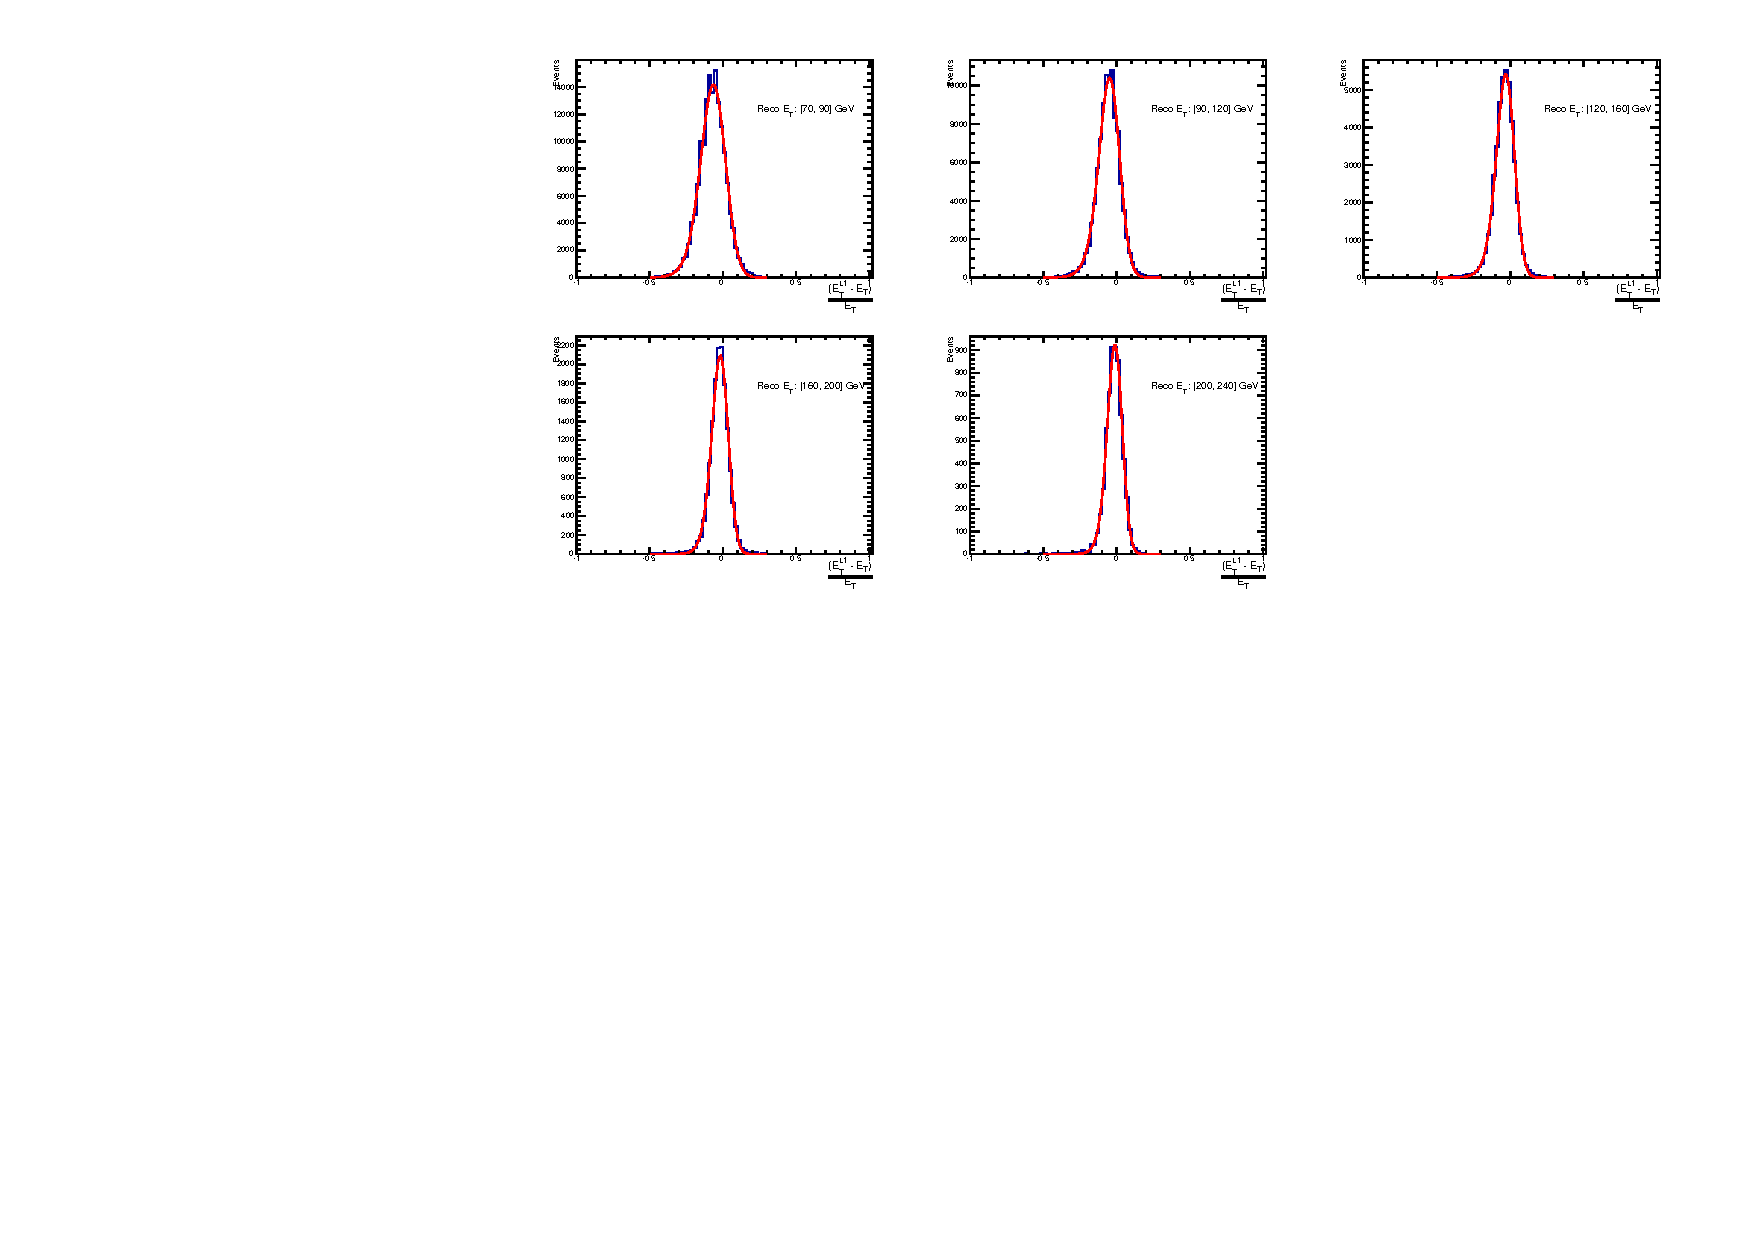
\includegraphics[width = 1.0\linewidth]{plots/calo_ptresolution_low.pdf}
   \centering (a)
     \end{minipage}
\end{figure}

\begin{figure}
    \centering
    \begin{minipage}[b]{0.98\linewidth}
    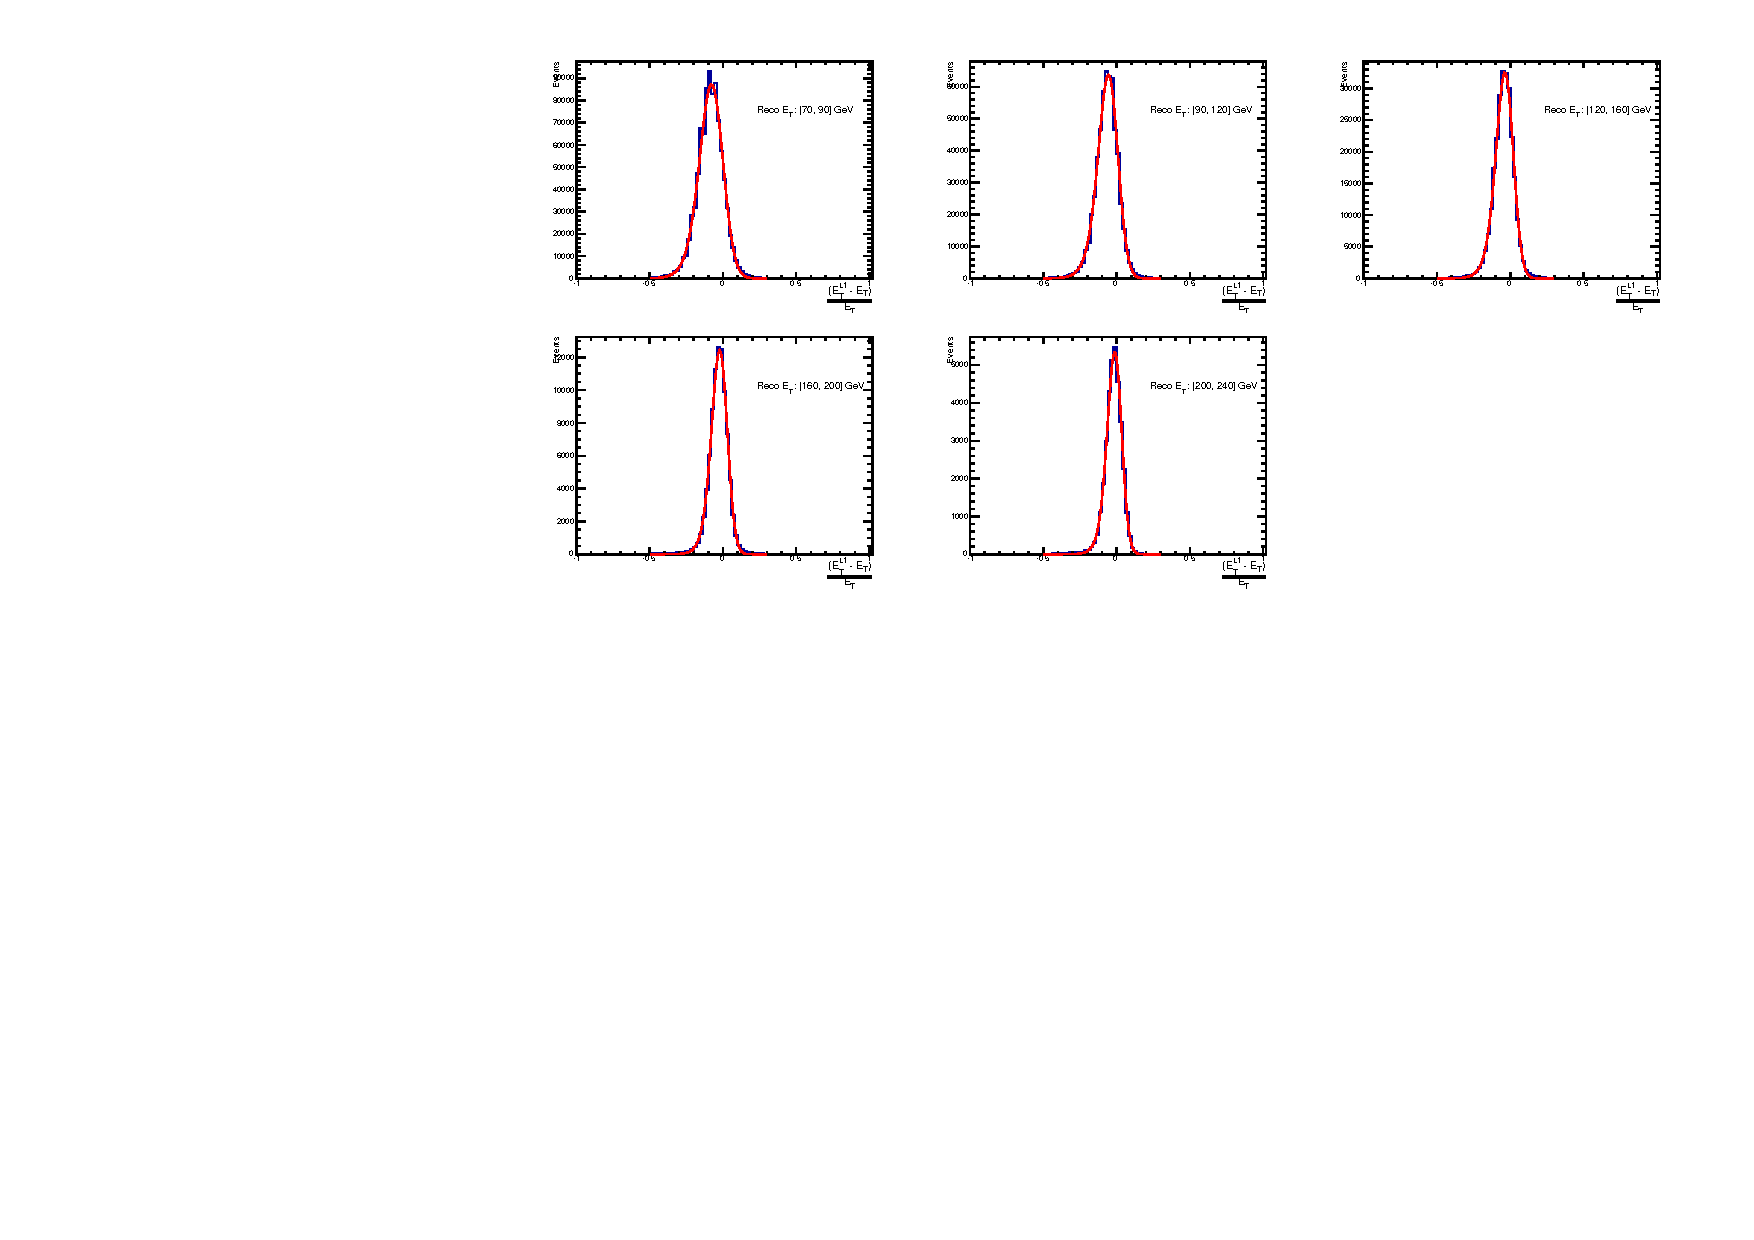
\includegraphics[width=1.0\textwidth]{plots/calo_ptresolution_medium.pdf}
    \centering (b)
    \end{minipage}
    \quad
    \begin{minipage}[b]{0.98\linewidth}
    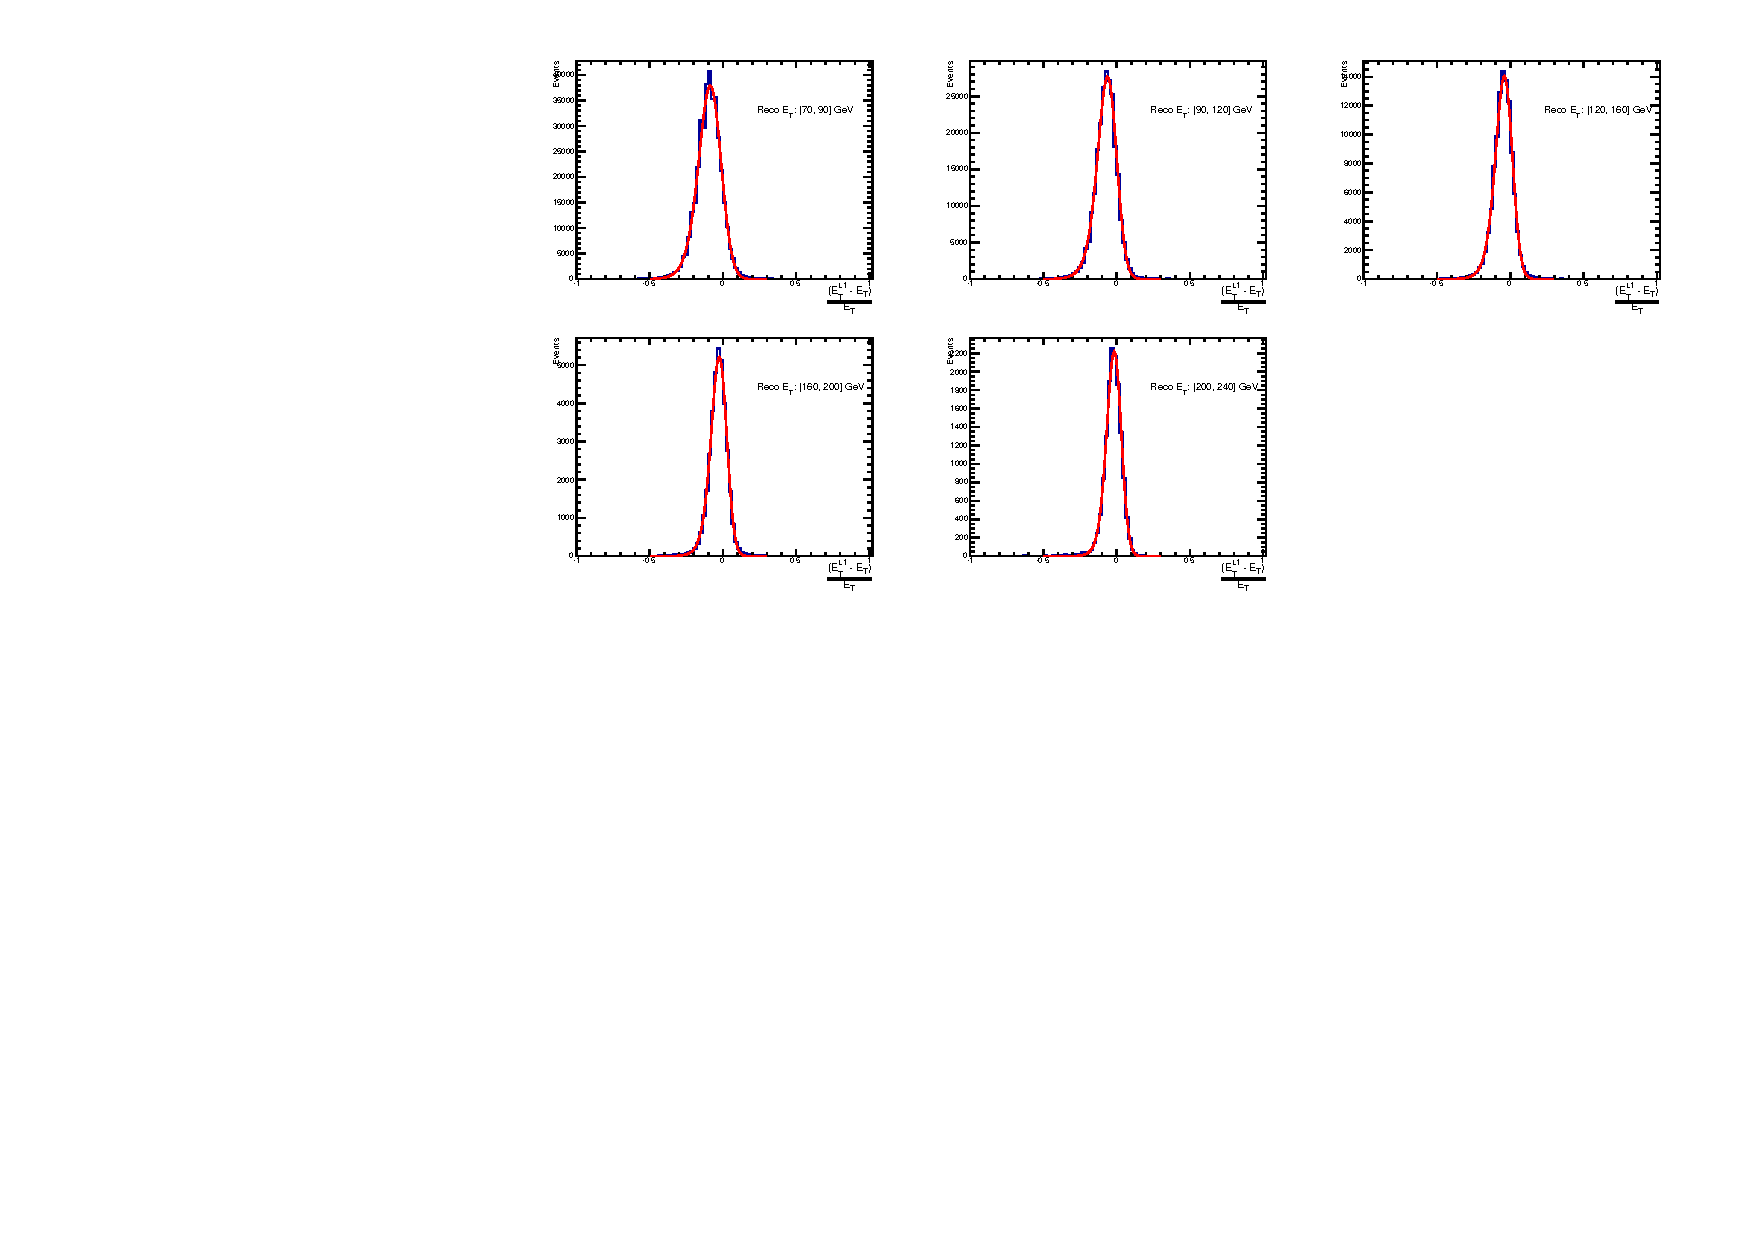
\includegraphics[width=1.0\textwidth]{plots/calo_ptresolution_high.pdf}
    \centering (c$)$ 
    \end{minipage}
     \caption[ Resolution plots of the leading offline \Calo $\et$ measured as a function of  $\frac{(\text{L1 E}_{T} -  \text{Offline E}_{T})}{\text{Offline E}_{T}}$ for  low (a), medium (b) and high (c) pile-up conditions.] { Resolution plots of the leading offline jet \Calo $\et$ measured as a function of  $\frac{(\text{L1 E}_{T} -  \text{Offline E}_{T})}{\text{Offline E}_{T}}$ for  low (a), medium (b) and high (c) pile-up conditions as defined in Section (\ref{subsec:l1jetseedpu}). }
\end{figure}

\begin{figure}[htpb]

    \centering
    \begin{minipage}[b]{0.98\linewidth}
    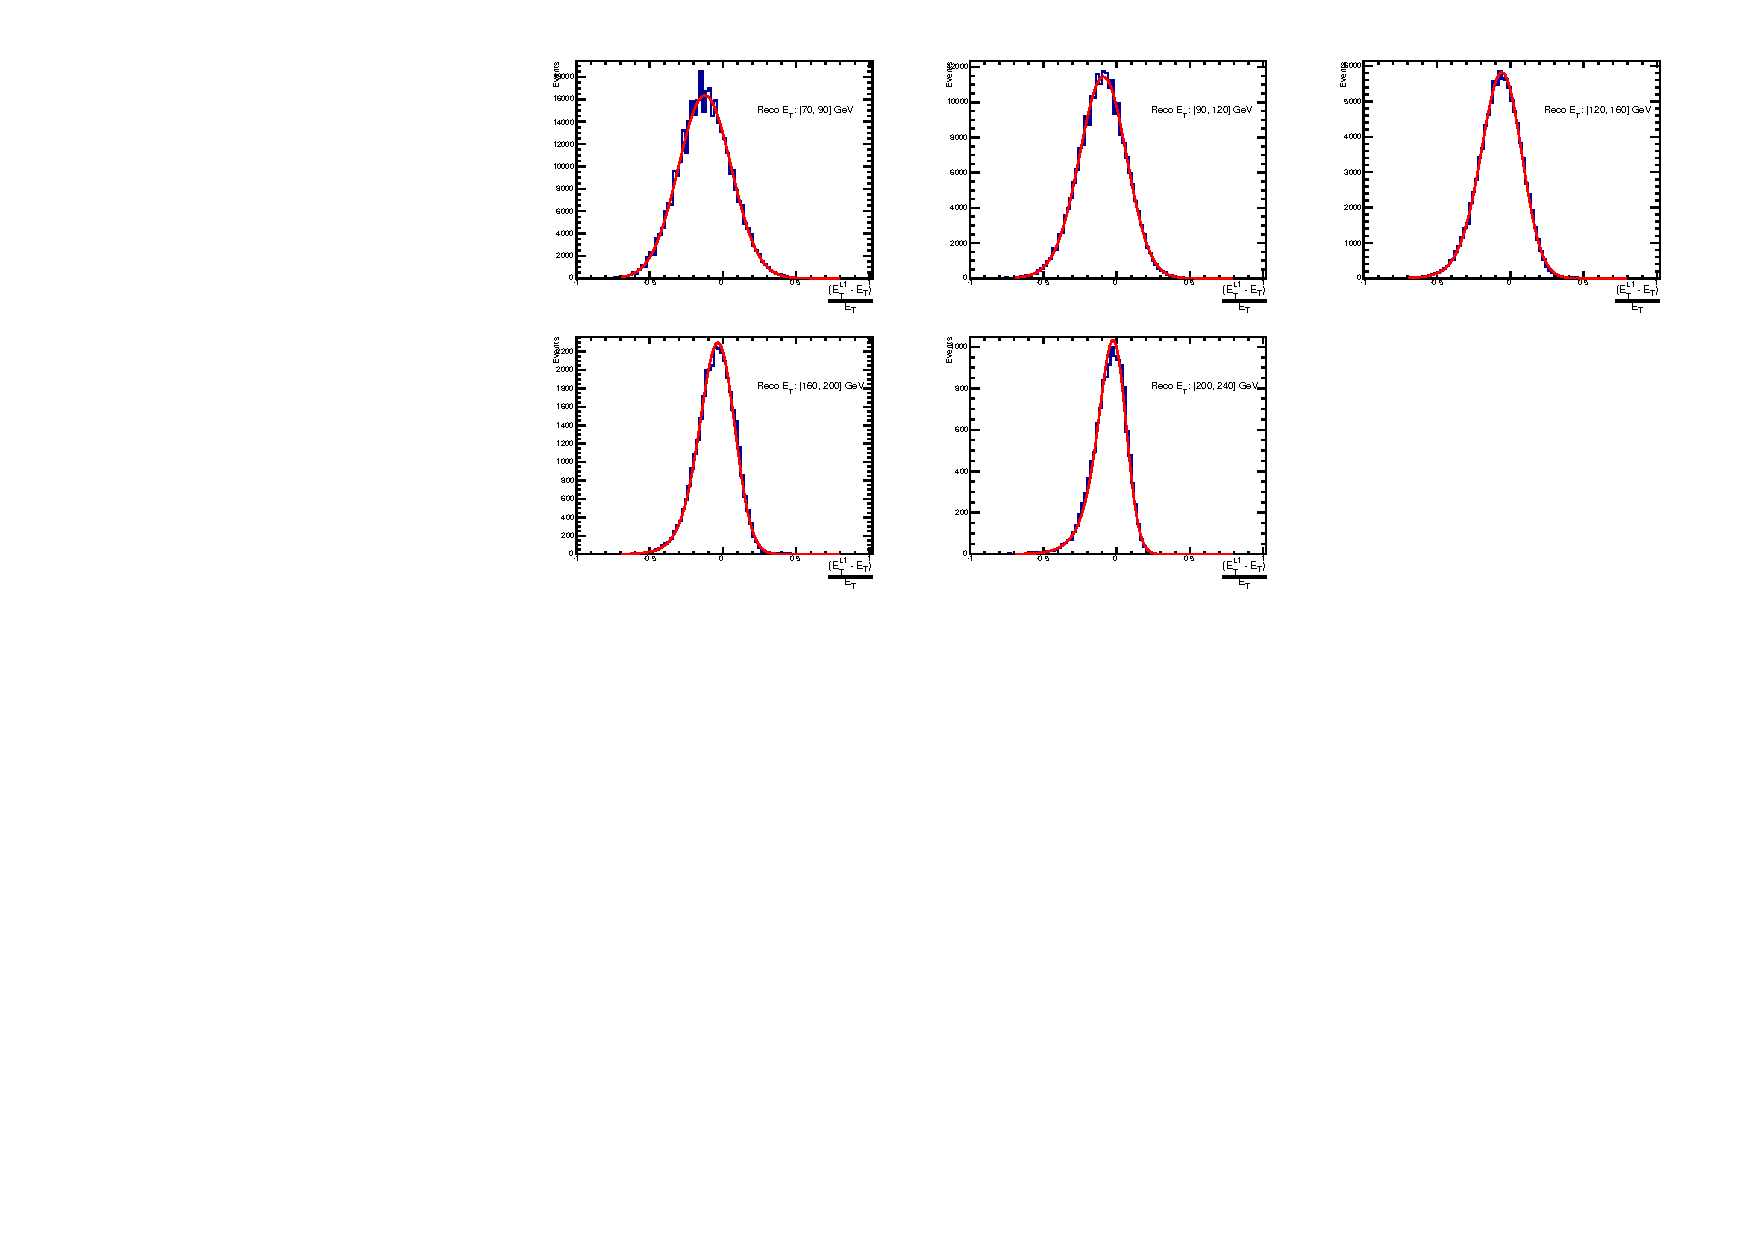
\includegraphics[width=1.0\textwidth]{plots/pf_ptresolution_low.pdf}
    \centering (a)
    \end{minipage}
    \quad
    \begin{minipage}[b]{0.98\linewidth}
    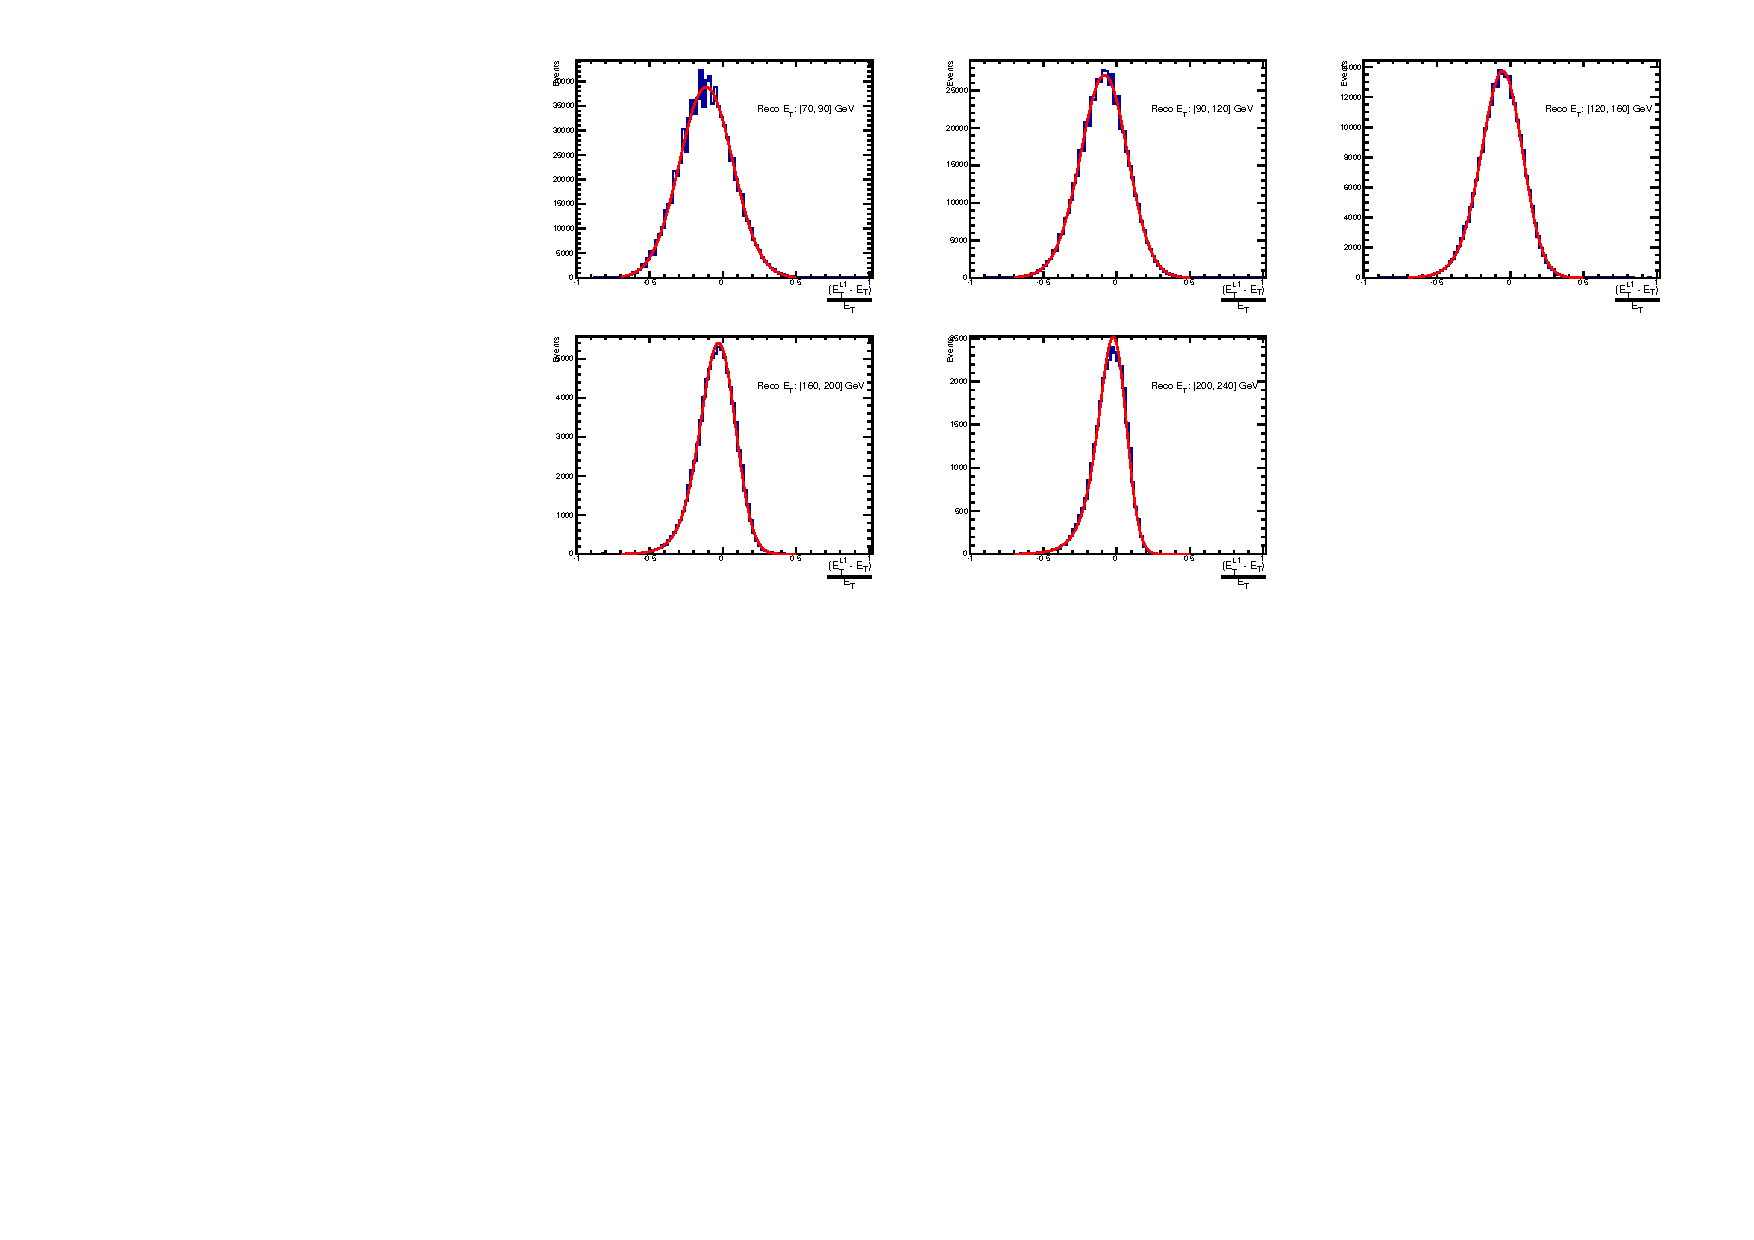
\includegraphics[width=1.0\textwidth]{plots/pf_ptresolution_medium.pdf}
    \centering (b) 
    \end{minipage}
\end{figure}

\begin{figure}
    \begin{minipage}[b]{0.98\linewidth}
    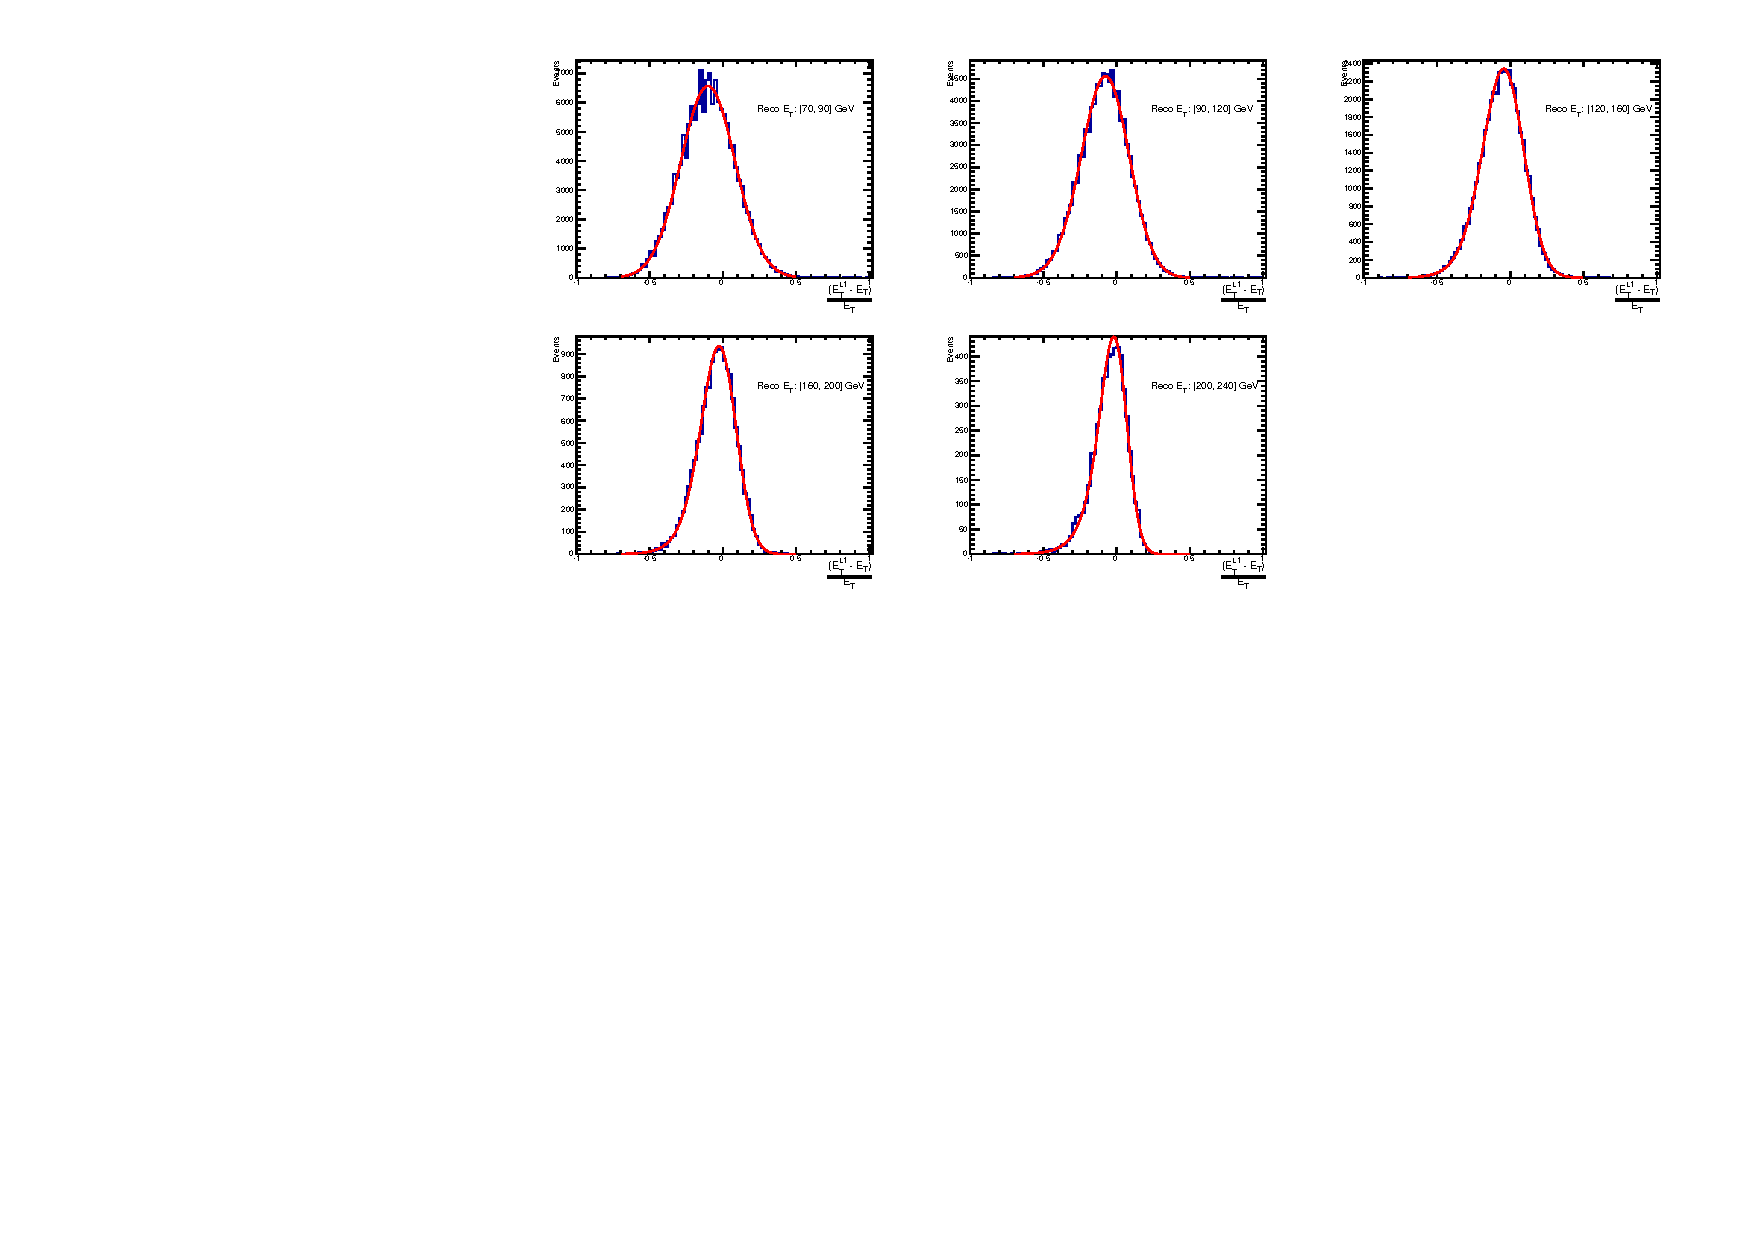
\includegraphics[width=1.0\textwidth]{plots/pf_ptresolution_high.pdf}
    \centering (c$)$ 
    \end{minipage}
      \caption[ Resolution plots of the leading off-line PF $\et$ measured as a function of  $\frac{(\text{L1 E}_{T} -  \text{Offline E}_{T})}{\text{Offline E}_{T}}$ for  low (a), medium (b) and high (c) pile-up conditions.] { Resolution plots of the leading offline jet \PF $\et$ measured as a function of  $\frac{(\text{L1 E}_{T} -  \text{Offline E}_{T})}{\text{Offline E}_{T}}$ for  low (a), medium (b) and high (c) pile-up conditions as defined in Section (\ref{subsec:l1jetseedpu}). }
\end{figure}


\newpage
\section{Resolution for Energy Sum Quantities}
\label{app:jetenergysums}

The following plots show the resolution parameters for energy sum quantities as a function of the quantity (q) itself. In this case, the $\mu$, $\sigma$ and $\lambda$ fit values to an \ac{EMG} function defined by Equation (\ref{eq:emg}) for each of the individual $\frac{(\text{L1 q } -  \text{Offline q})}{\text{Offline q}}$ distributions, in bins of the quantity (q) is displayed. 


\begin{figure}[h!]
  \vspace{20pt}
        \centering
        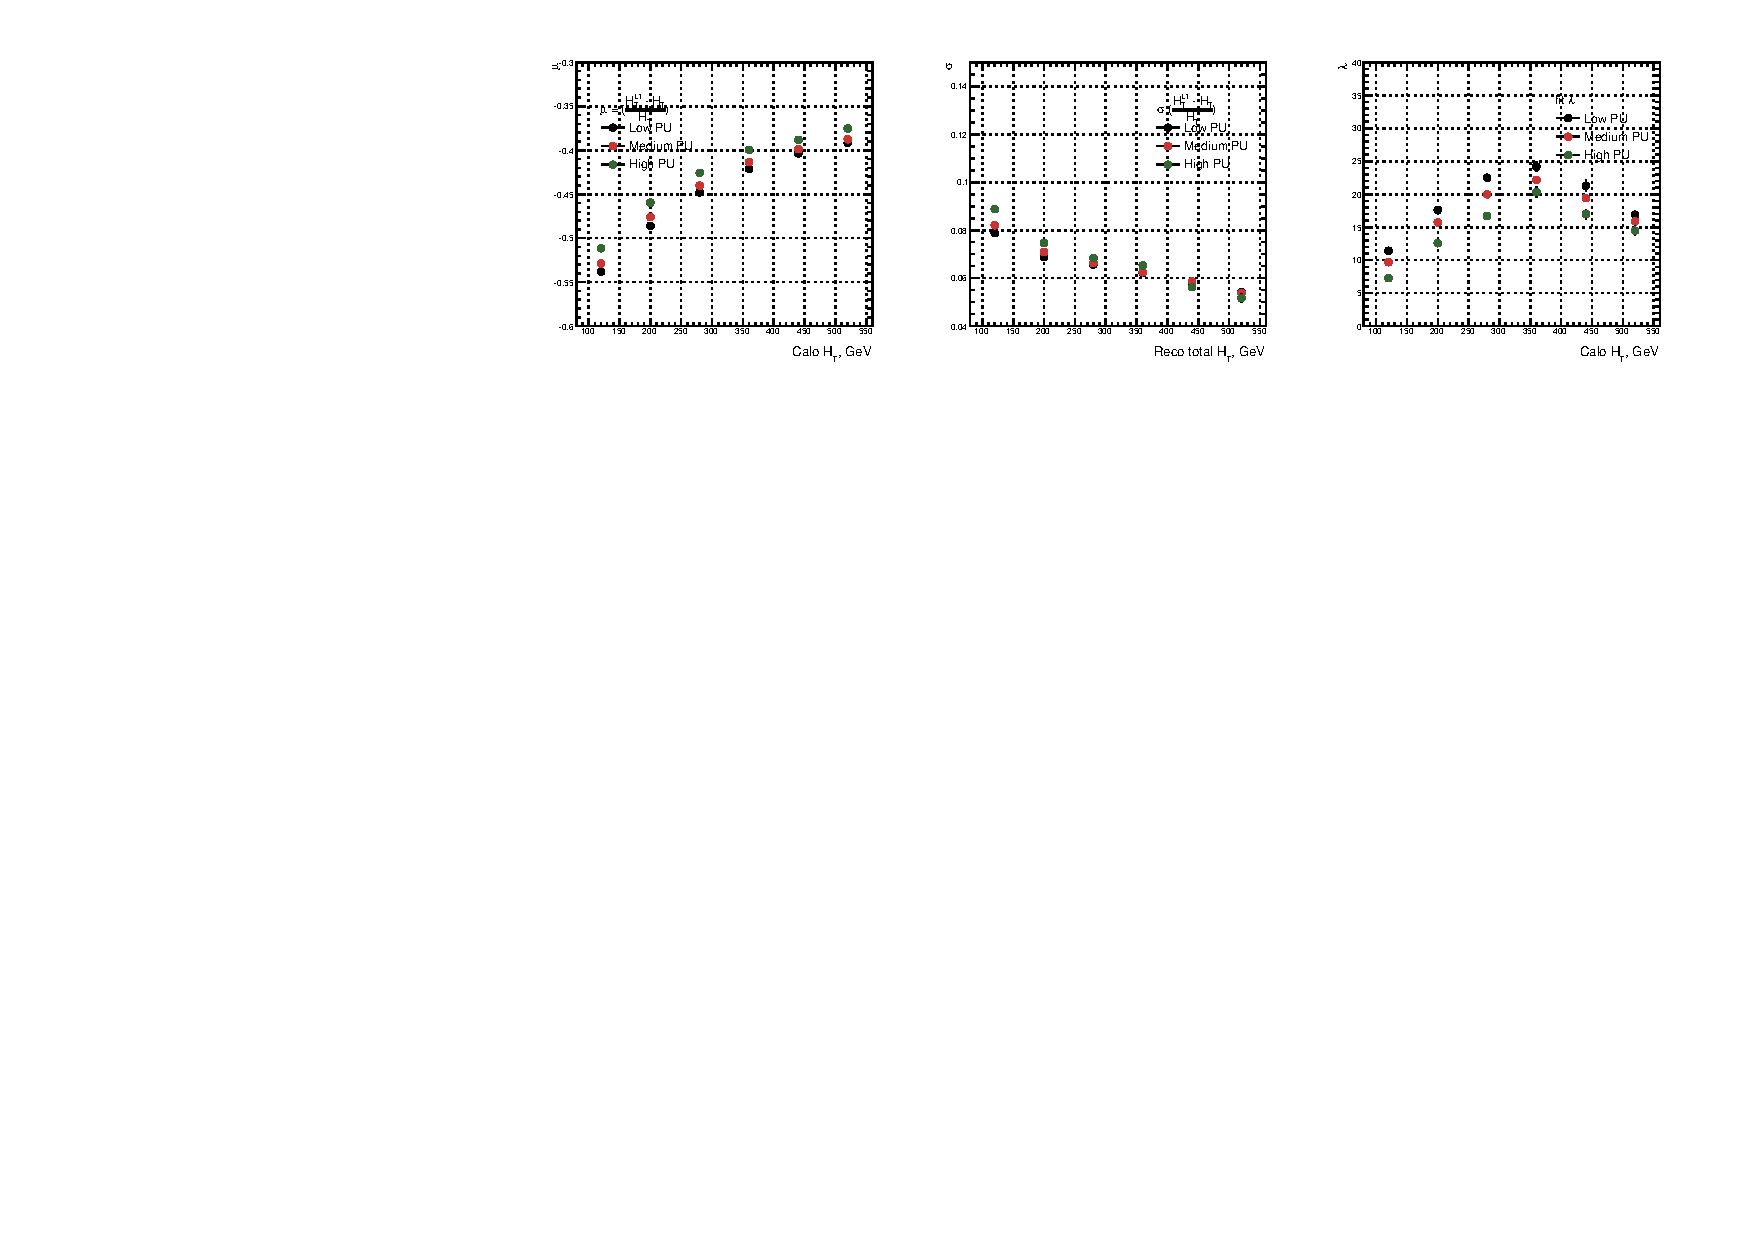
\includegraphics[width=1.0\textwidth]{plots/res_CaloHT_summary_v2.pdf}
        \caption[$\theht$~resolution parameters in bins of Calo $\theht$~measured in the defined low, medium and high pile up conditions.]{$\theht$~resolution parameters in bins of Calo $\theht$~measured for the defined low, medium and high pile-up conditions. Shown are the mean $\mu$ (left), resolution $\sigma$ (middle) and $\lambda$ (right) fit values to an \ac{EMG} function for the $\frac{(L1 \theht - \theht)}{\theht}$ distributions.}
        \label{fig:calohtresultspu}
\end{figure}
\begin{figure}[h!]
  \vspace{20pt}
        \centering
        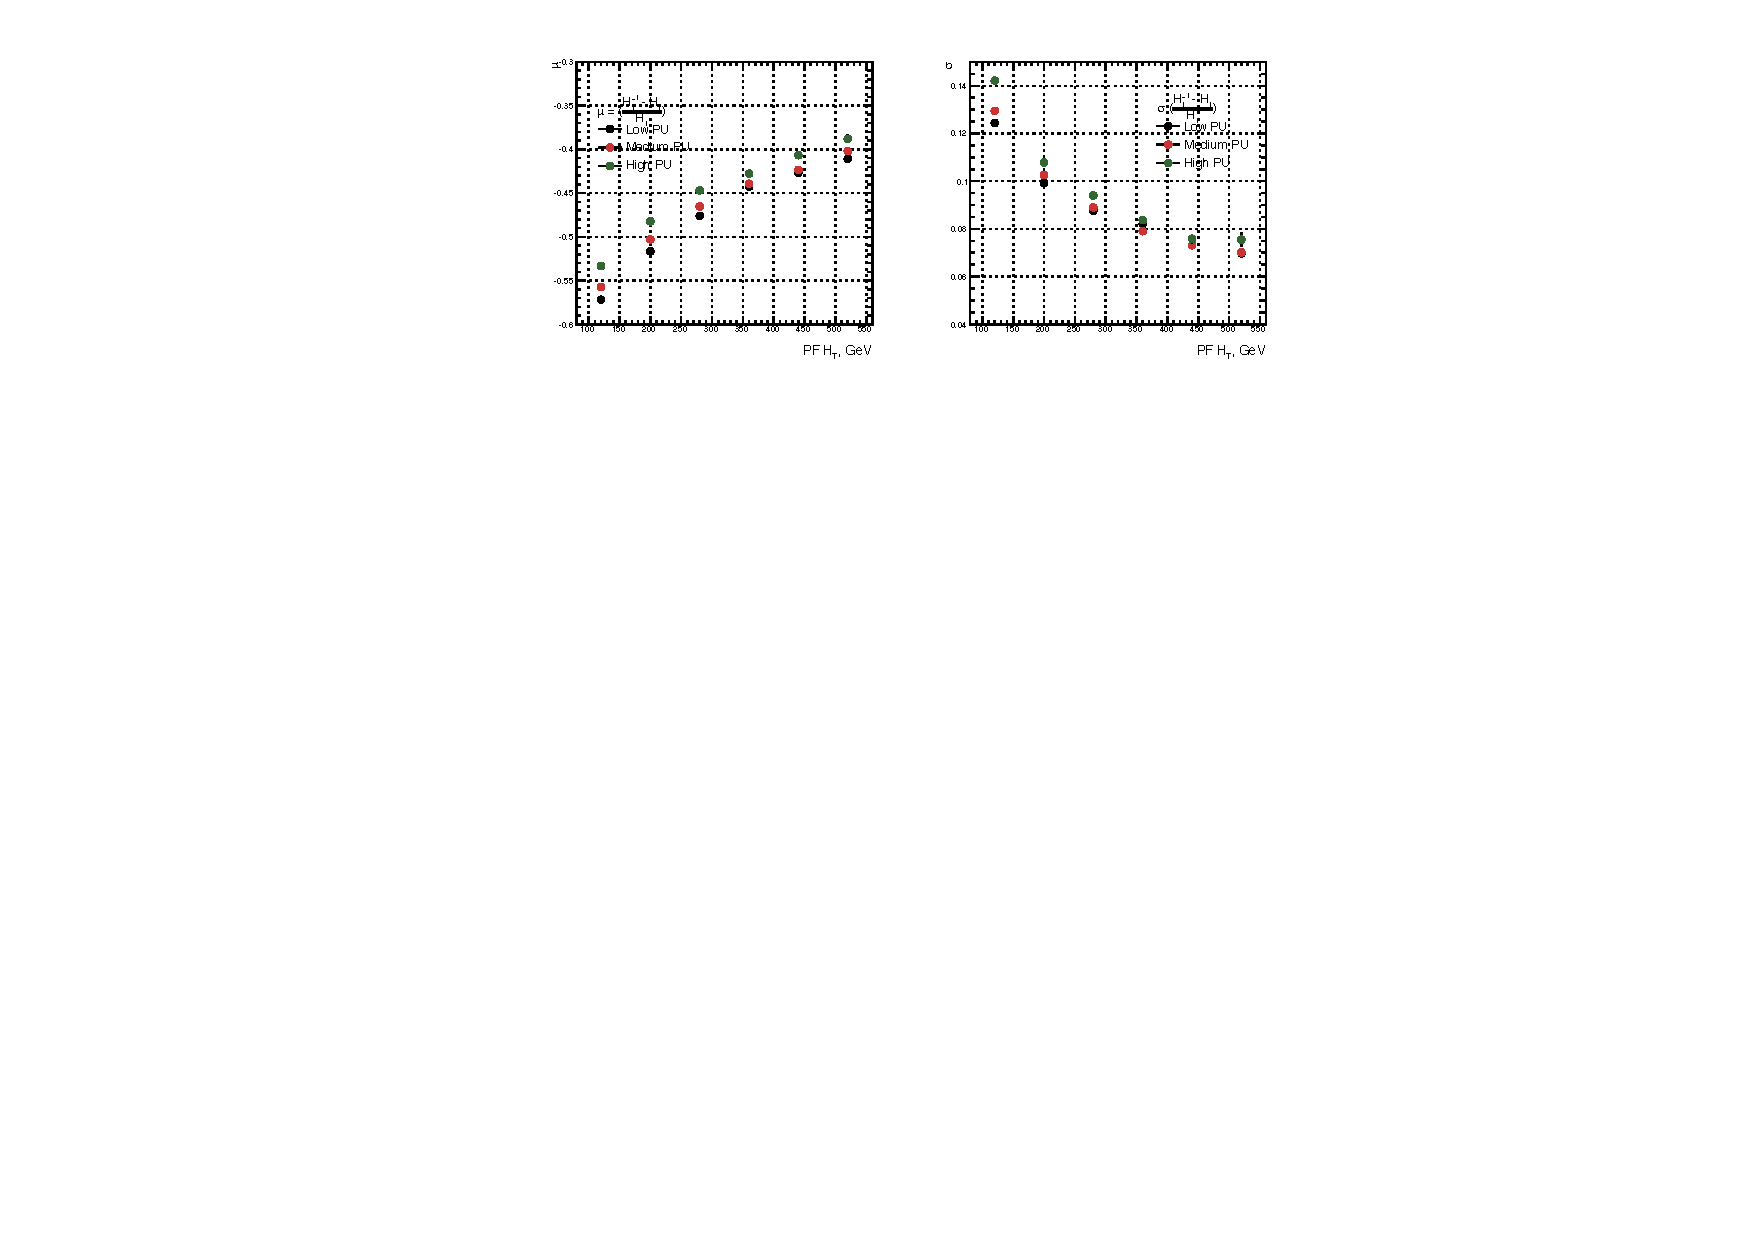
\includegraphics[width=1.0\textwidth]{plots/res_pfHT_summary_v2.pdf}
        \caption[$\theht$~resolution parameters in bins of PF $\theht$~measured in the defined low, medium and high pile up conditions.]{$\theht$~resolution parameters in bins of PF $\theht$~measured for the defined low, medium and high pile-up conditions. Shown are the mean $\mu$ (left), resolution $\sigma$ (middle) and $\lambda$ (right) fit values to an \ac{EMG} function for the $\frac{(L1 \theht - \theht)}{\theht}$ distributions.}
        \label{fig:pfhtresultspu}
\end{figure}

\begin{figure}[h!]
  \vspace{20pt}
        \centering
        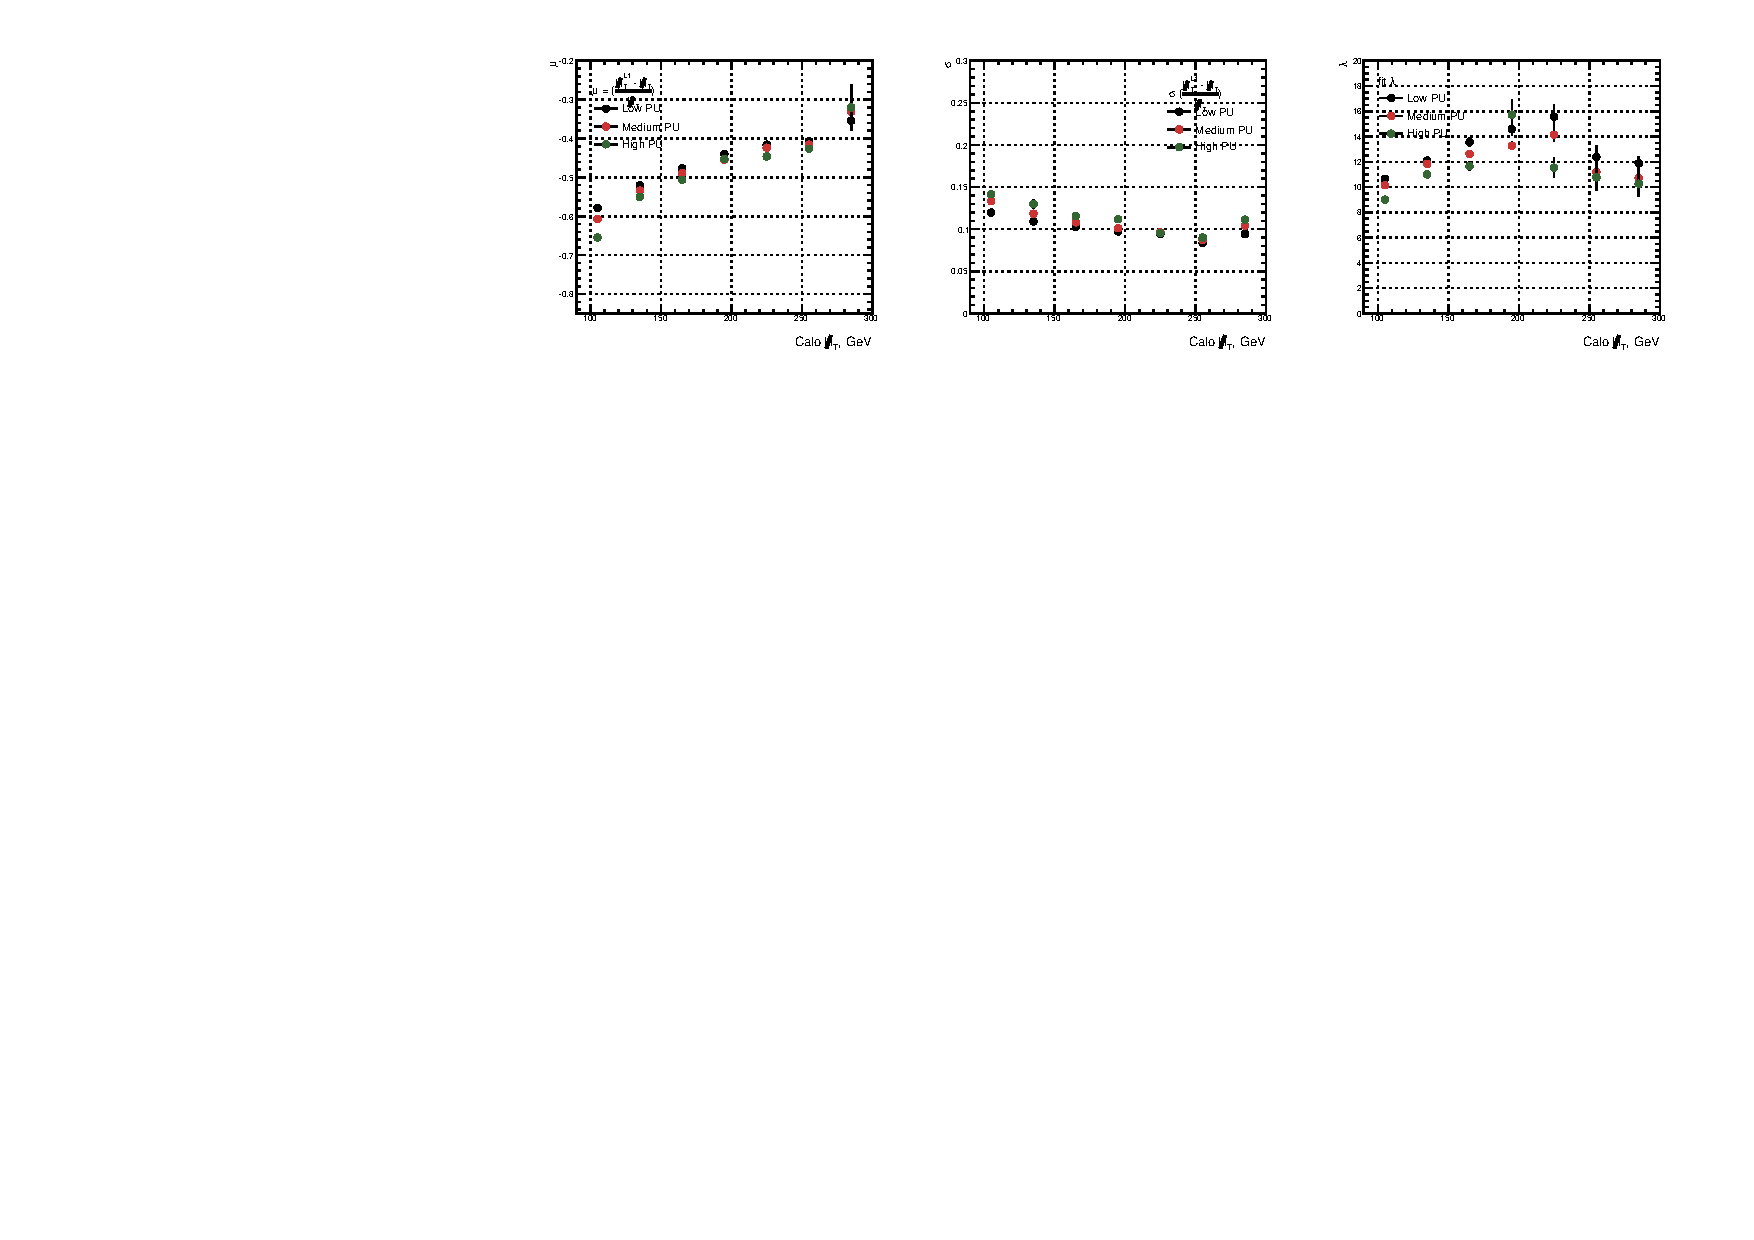
\includegraphics[width=1.0\textwidth]{plots/res_CaloMHT_summary_v2.pdf}
        \caption[$\mht$~resolution parameters in bins of $\mht$~measured in the defined low, medium and high pile up conditions.]{$\mht$~resolution parameters in bins of $\mht$~measured for the defined low, medium and high pile-up conditions. Shown are the mean $\mu$ (left), resolution $\sigma$ (middle) and $\lambda$ (right) fit values to an \ac{EMG} function for the $\frac{(L1 \mht - \mht)}{\mht}$ distributions.}
        \label{fig:calomhtresultspu}
\end{figure}
\begin{figure}[h!]
  \vspace{20pt}
        \centering
        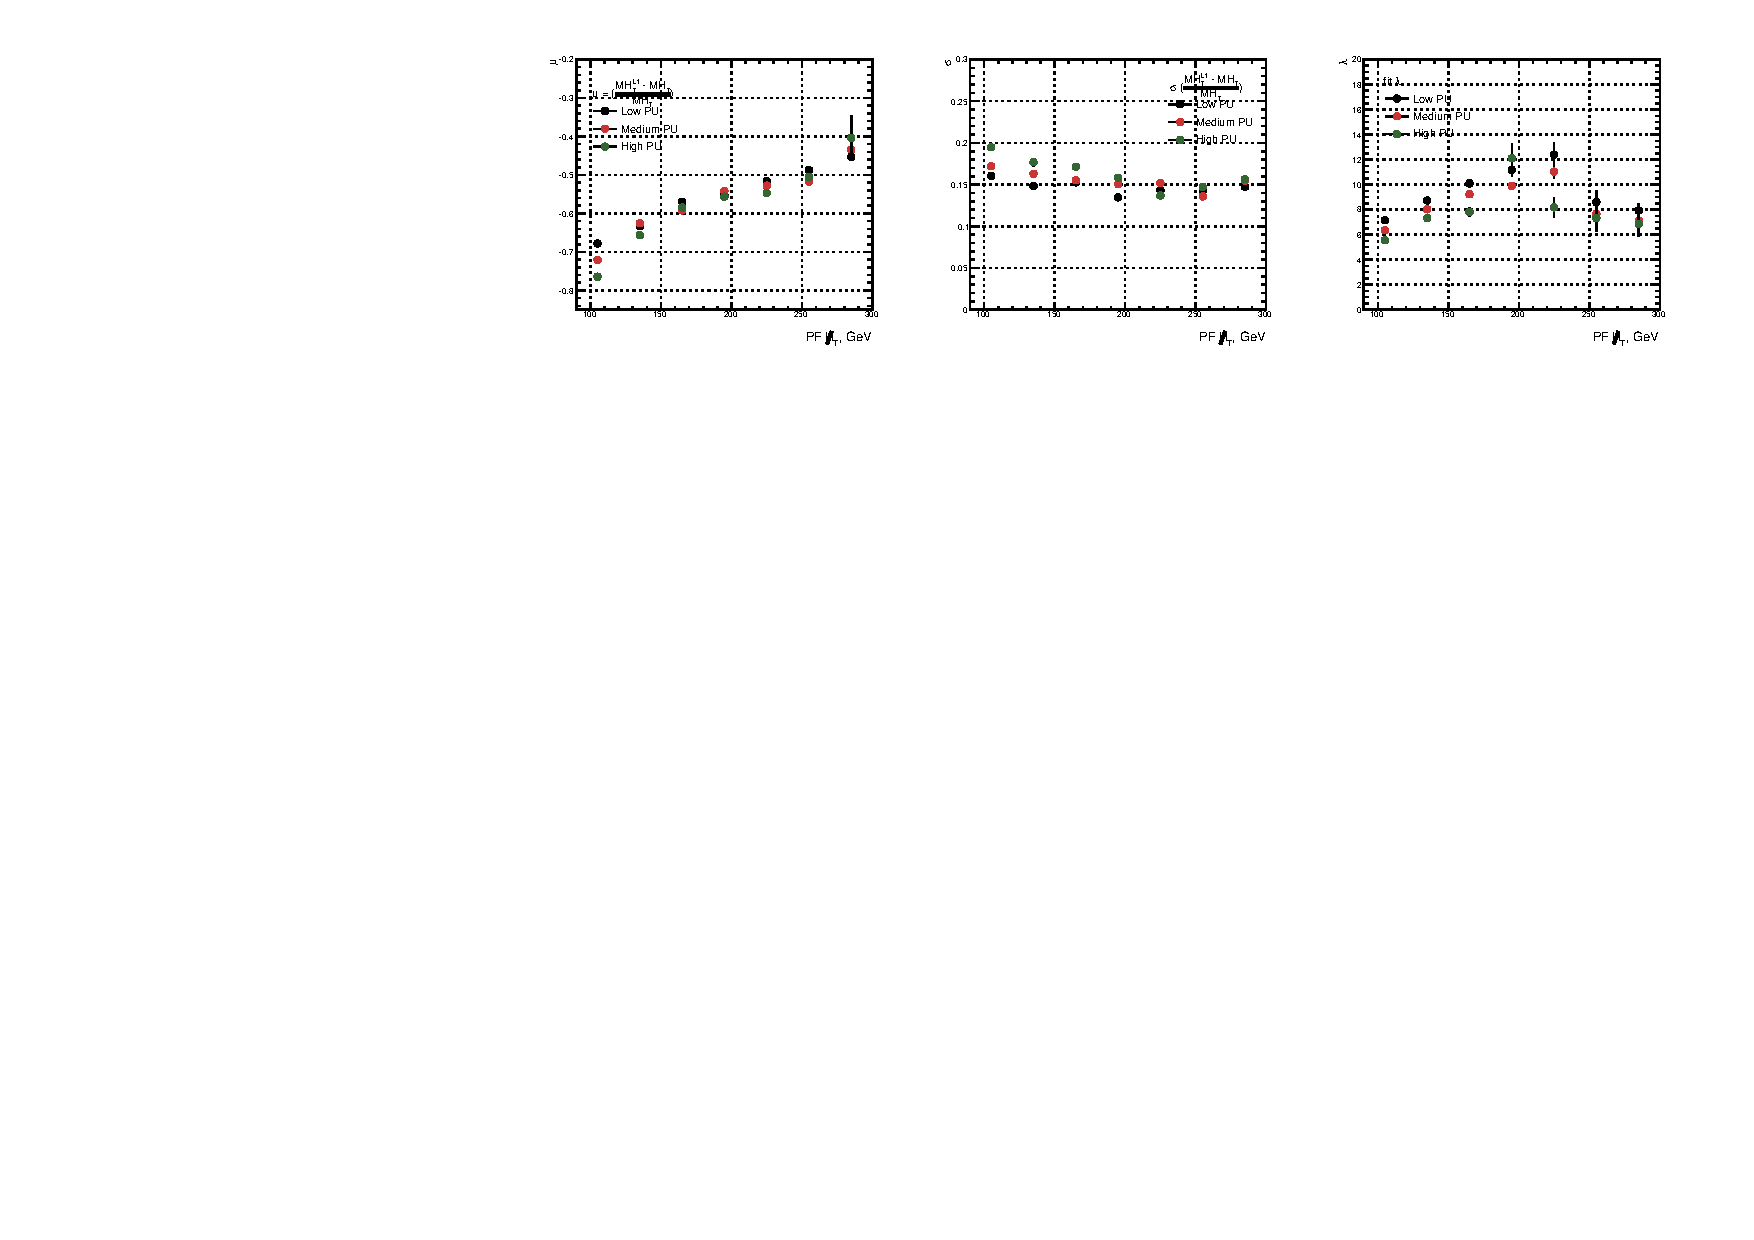
\includegraphics[width=1.0\textwidth]{plots/res_pfMHT_summary_v2.pdf}
        \caption[$\mht$~resolution parameters in bins of PF $\mht$~measured in the defined low, medium and high pile up conditions.]{$\mht$~resolution parameters in bins of PF $\mht$~measured for the defined low, medium and high pile-up conditions. Shown are the mean $\mu$ (left), resolution $\sigma$ (middle) and $\lambda$ (right) fit values to an \ac{EMG} function for the $\frac{(L1 \mht - \mht)}{\mht}$ distributions.} \label{fig:pfmhtresultspu}
\end{figure}

\chapter{Additional material on background estimation methods}
\label{app:backgroundestimation}
\section{Determination of $k_{QCD}$}
\label{app:kqcd}


\begin{minipage}{\linewidth}
\centering
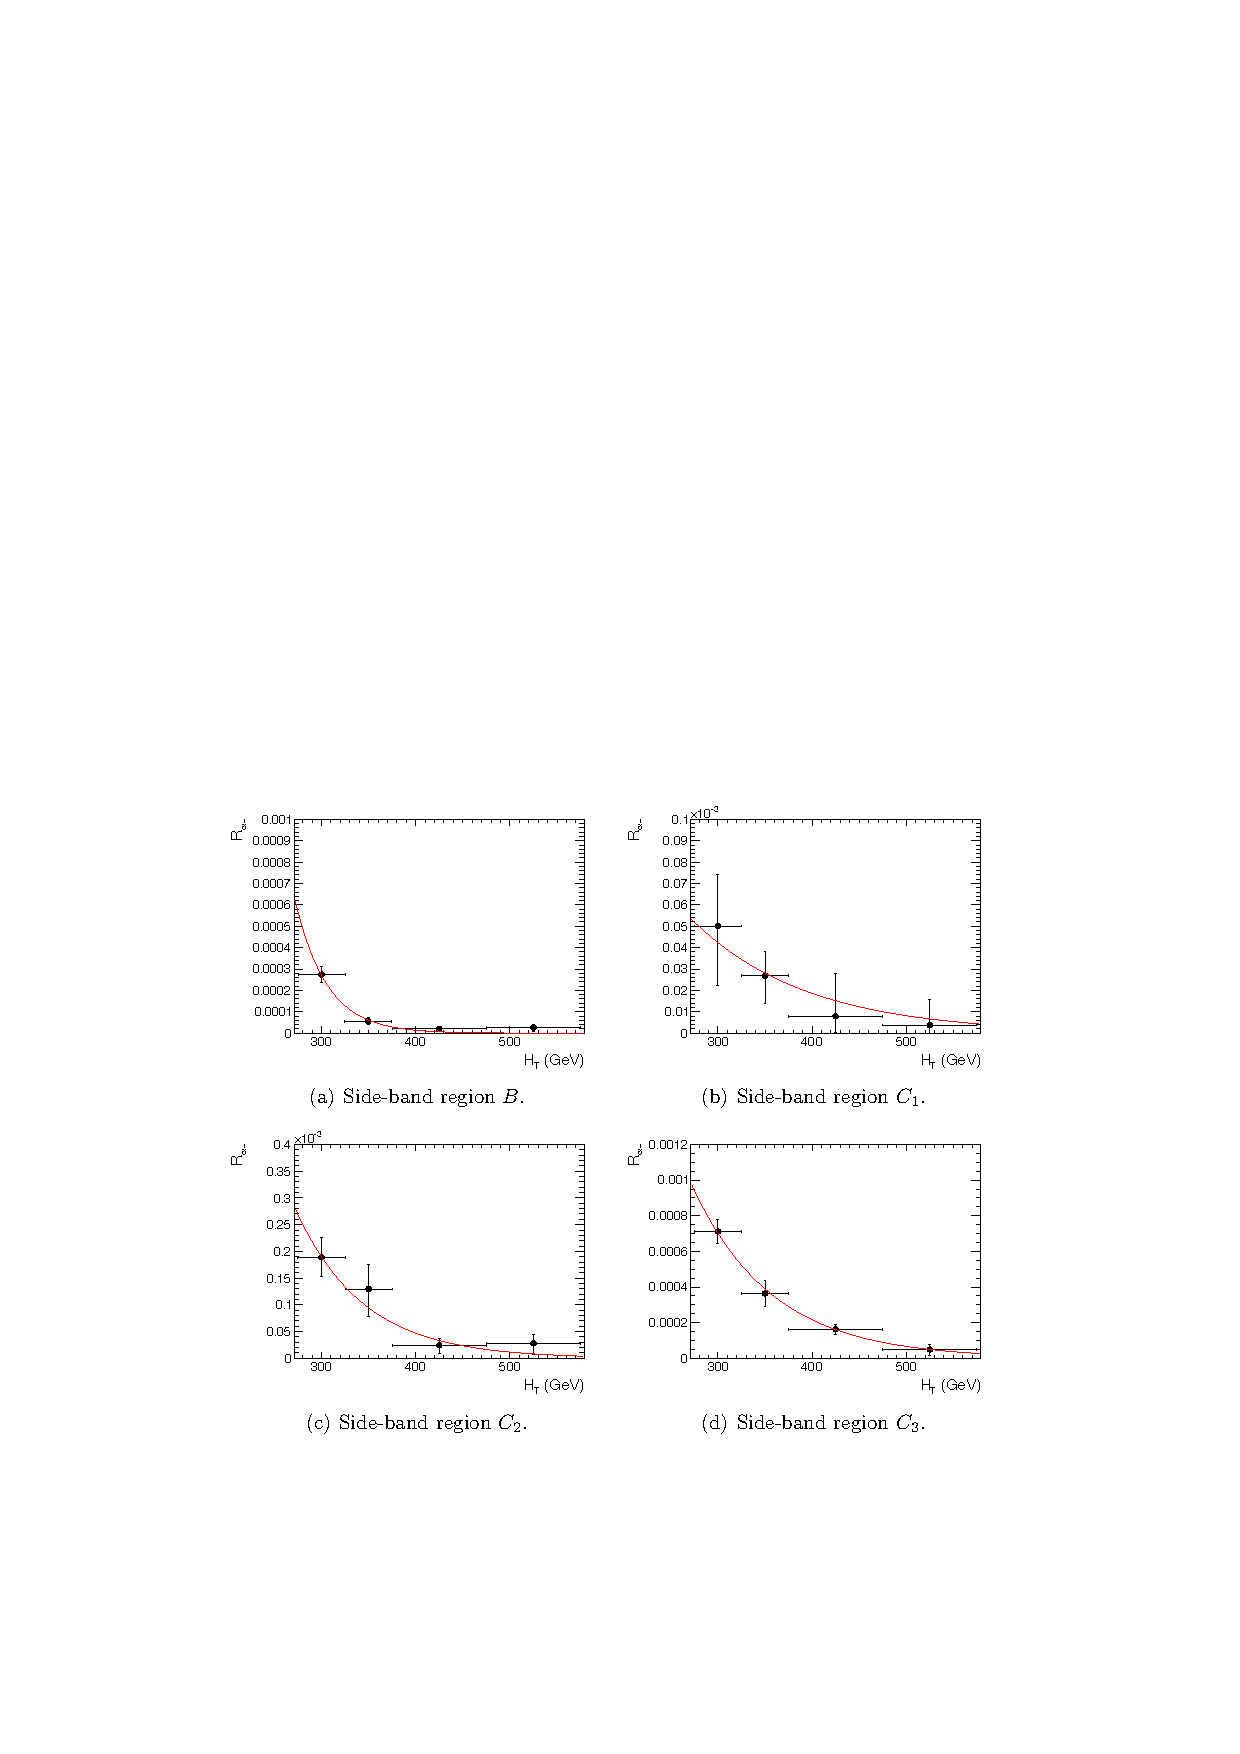
\includegraphics[width = 4.9in]{plots/qcd_sideband_fits.pdf}
\captionof{figure}[$R_{\alphat}$(\theht) and exponential fits for each of the data sideband regions. Fit is conducted between the \theht region 275 $<$ \theht $<$ 575.]{$R_{\alphat}$(\theht) and exponential fits for each of the data sideband regions. Fit is conducted between the \theht region 275 $<$ \theht $<$ 575.}
\label{fig:qcd_sideband_fits}
\end{minipage}

\section{Effect of Varying Background Cross-sections on Closure Tests }
\label{app:xsecvariation}

Closure tests with cross section variations of +20\% and -20\% applied to W + jets and \ttbar processes respectively.

\begin{figure}[ht]
\centering
\begin{minipage}[b]{0.48 \linewidth}
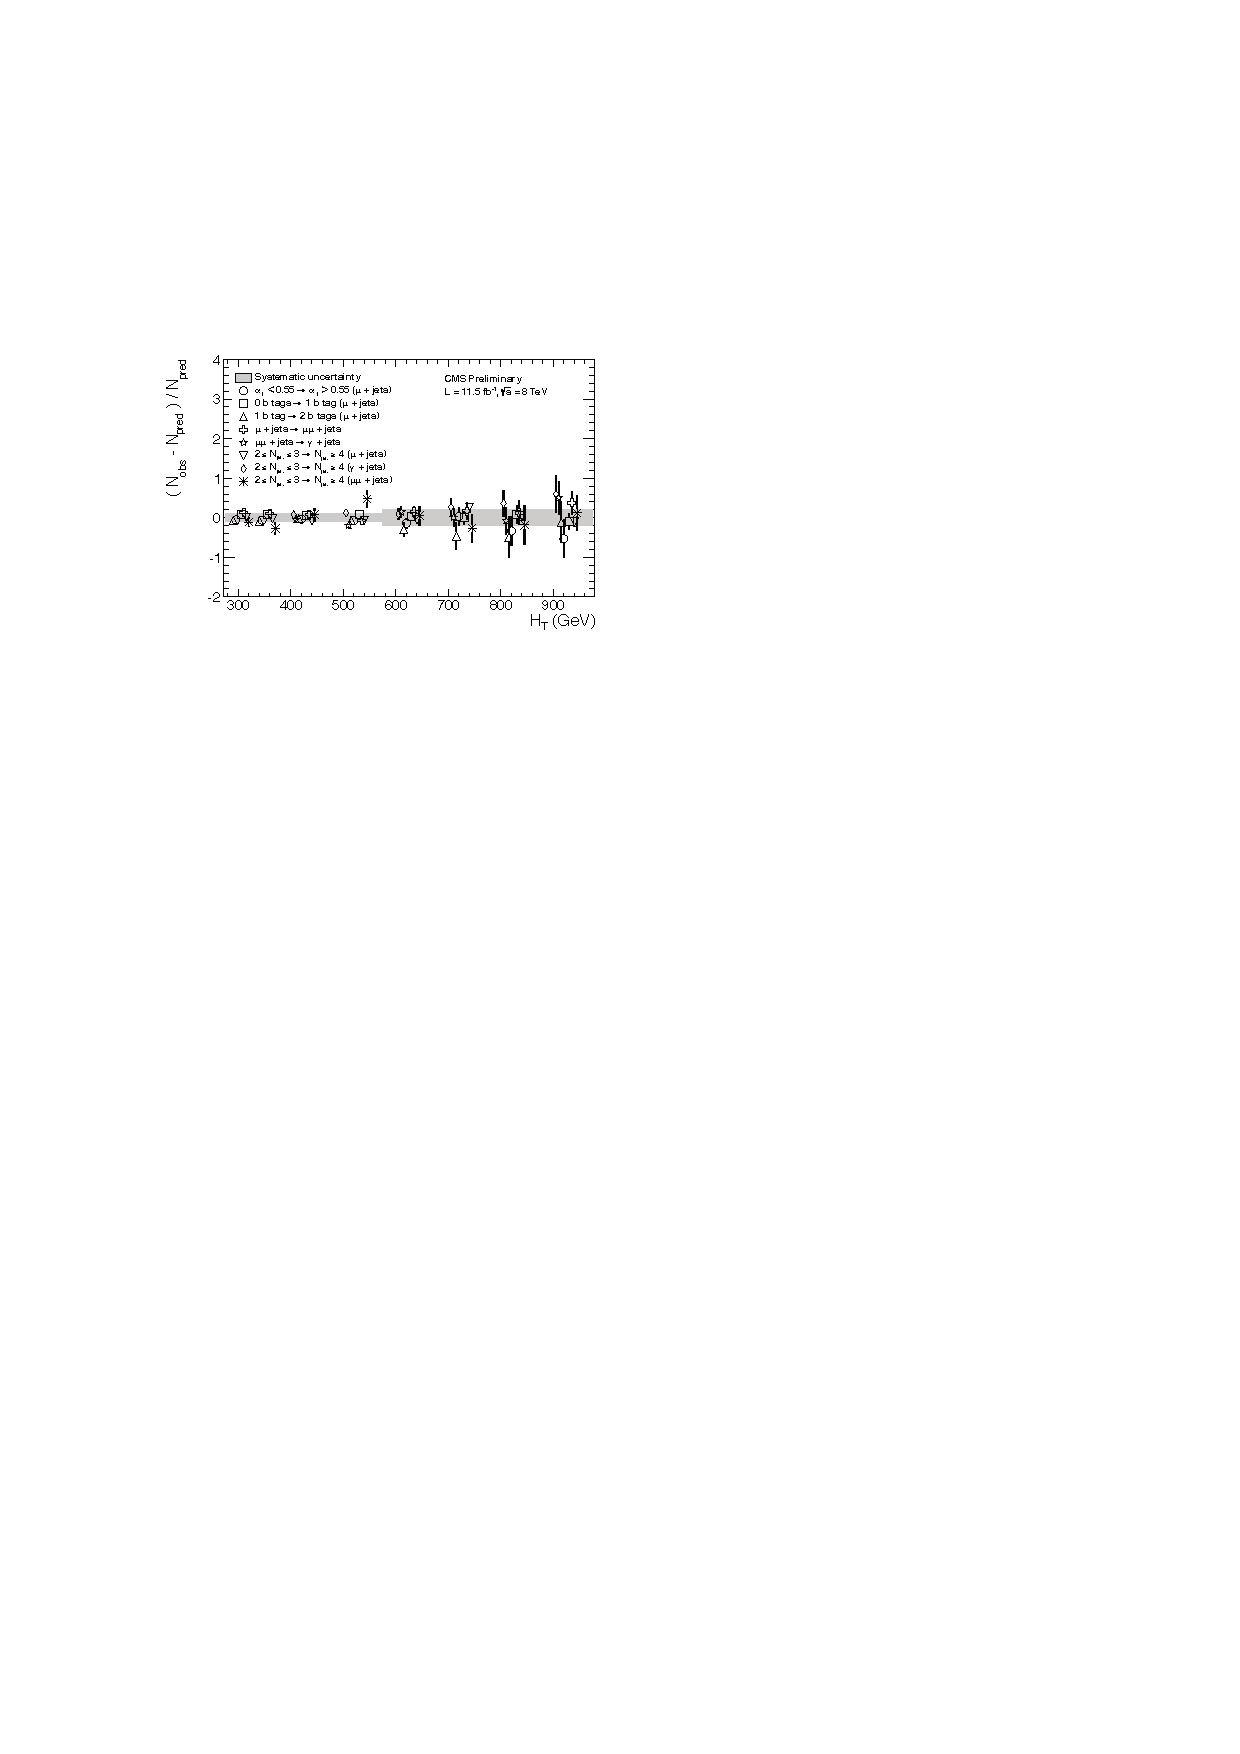
\includegraphics[width = 1.0\linewidth]{plots/syst-le3j_nominal.pdf}
\centering
(a)  
\end{minipage}
\quad
\begin{minipage}[b]{0.48\linewidth}
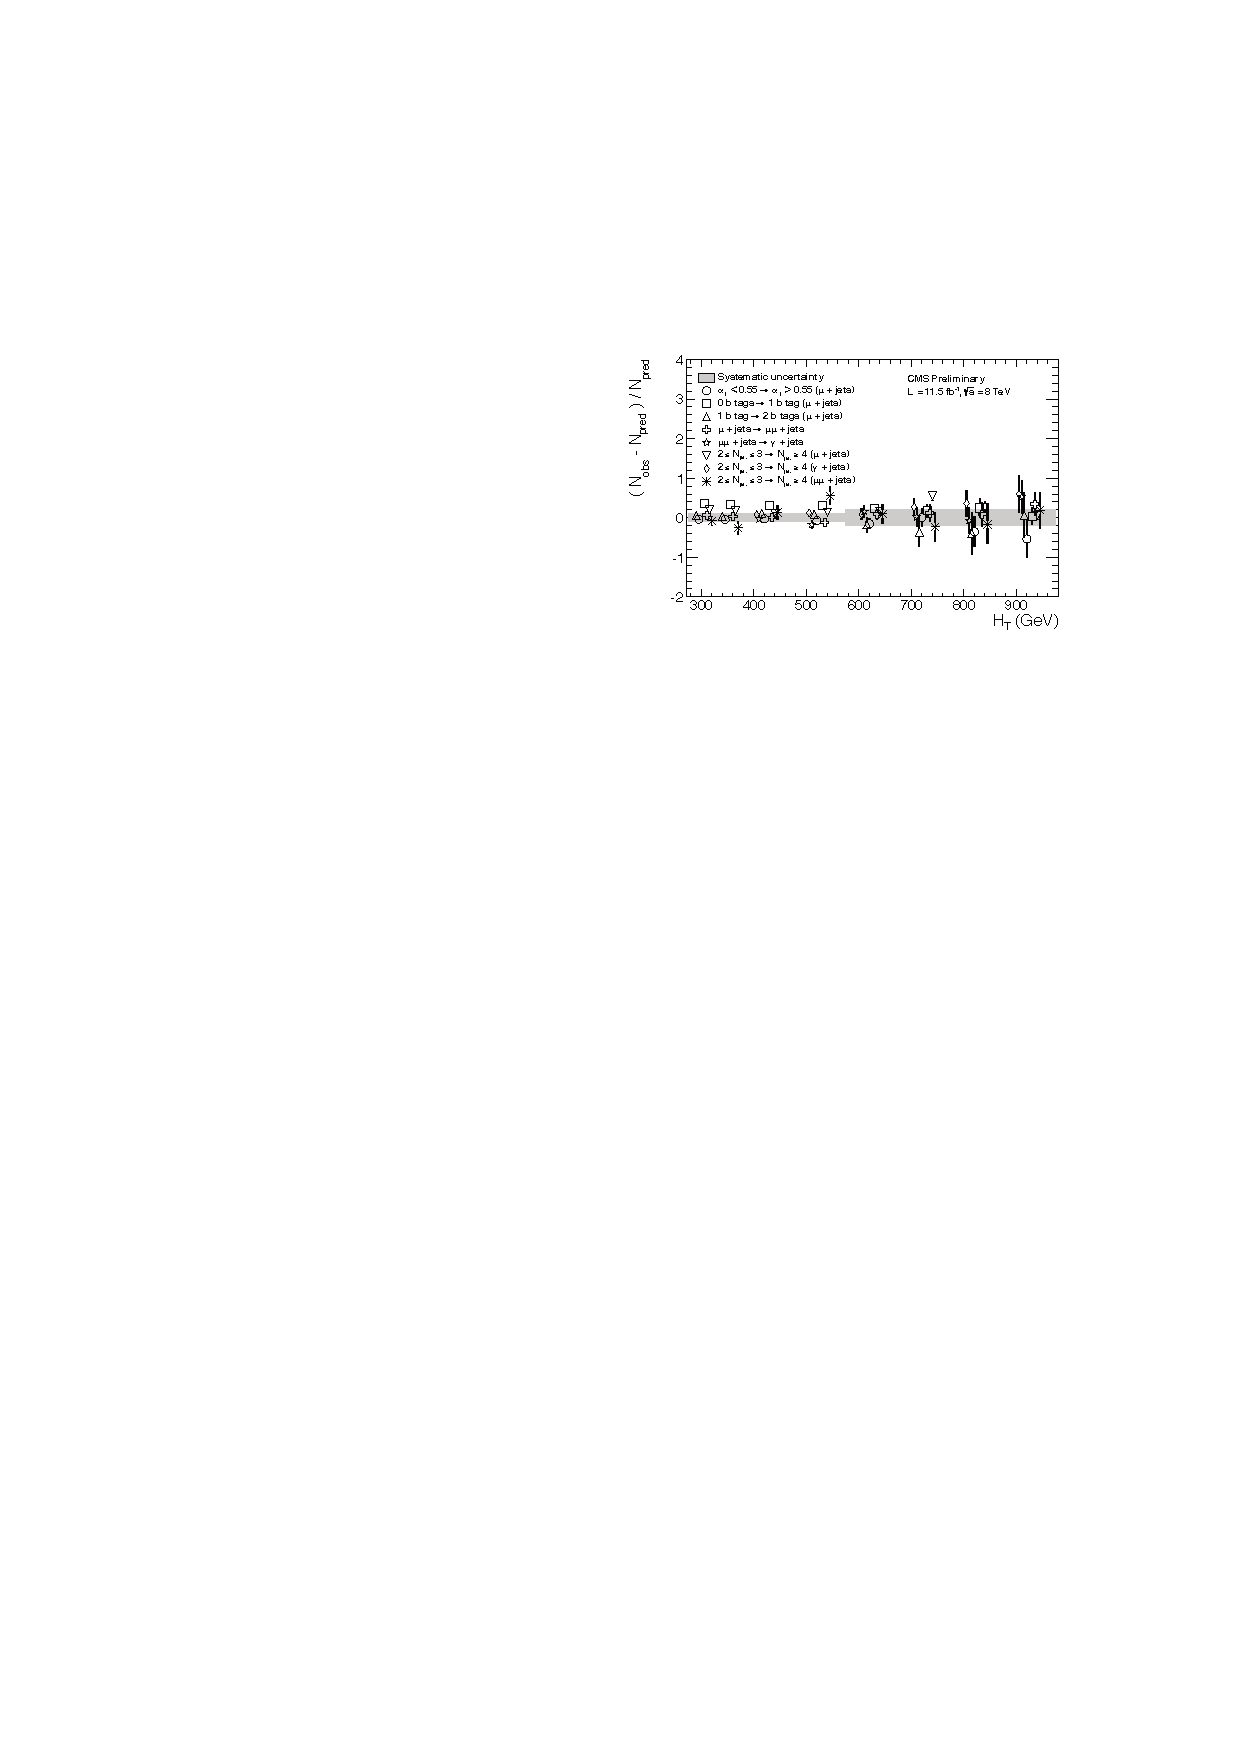
\includegraphics[width = 1.0\linewidth]{plots/syst-le3j_varied.pdf}
\centering
(b) 
\end{minipage}
\caption[Sets of closure tests overlaid on top of the systematic uncertainty used for each of the five \theht regions.]{Sets of closure tests (open symbols) overlaid on top of the systematic uncertainty used for each of the five \theht regions (shaded bands) and for the two different jet multiplicity bins (a) $2 \leq n_{jet} \leq 3$ and (b) $n_{jet} \geq 4$.}
\label{fig:xsecvariedle3j}
\end{figure}


\begin{figure}[ht]
\centering
\begin{minipage}[b]{0.48 \linewidth}
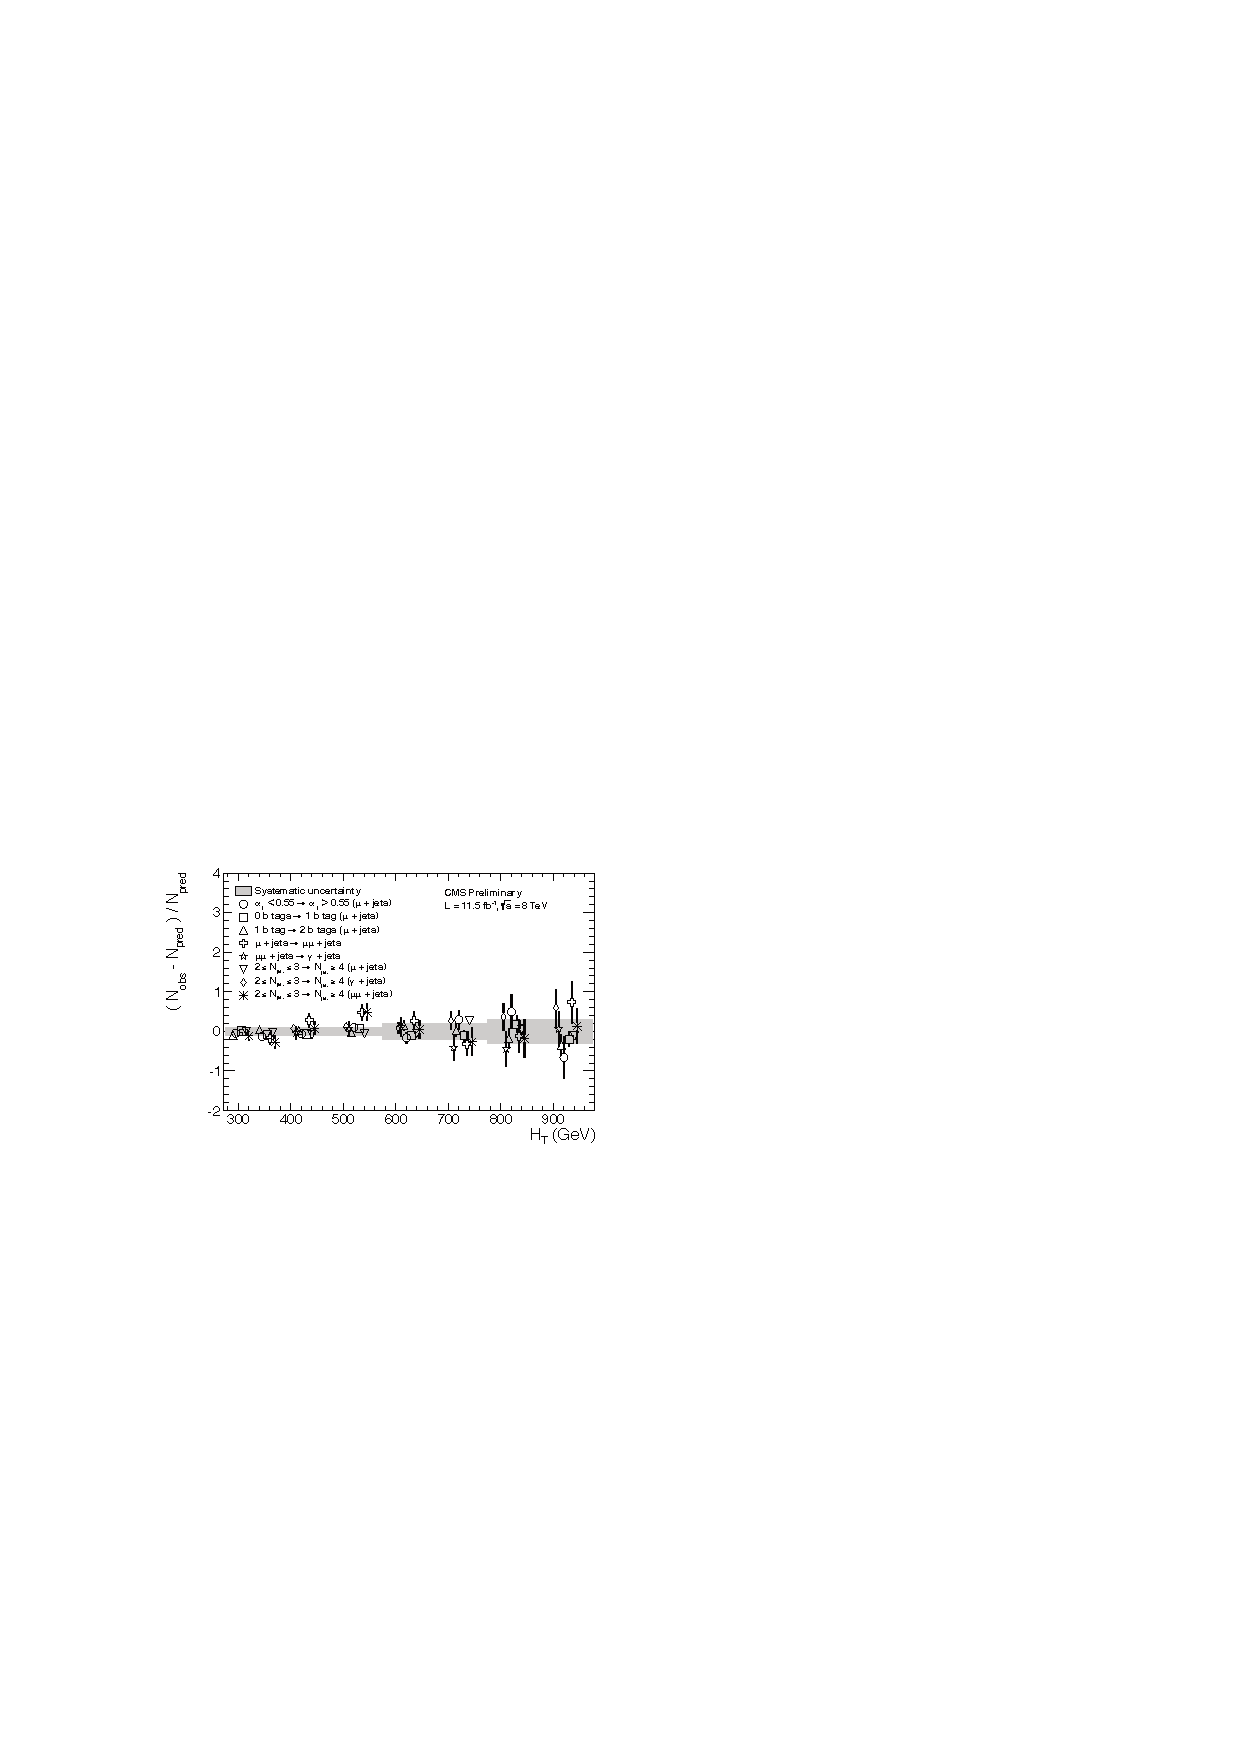
\includegraphics[width = 1.0\linewidth]{plots/syst-ge4j_nominal.pdf}
\centering
(a)  
\end{minipage}
\quad
\begin{minipage}[b]{0.48\linewidth}
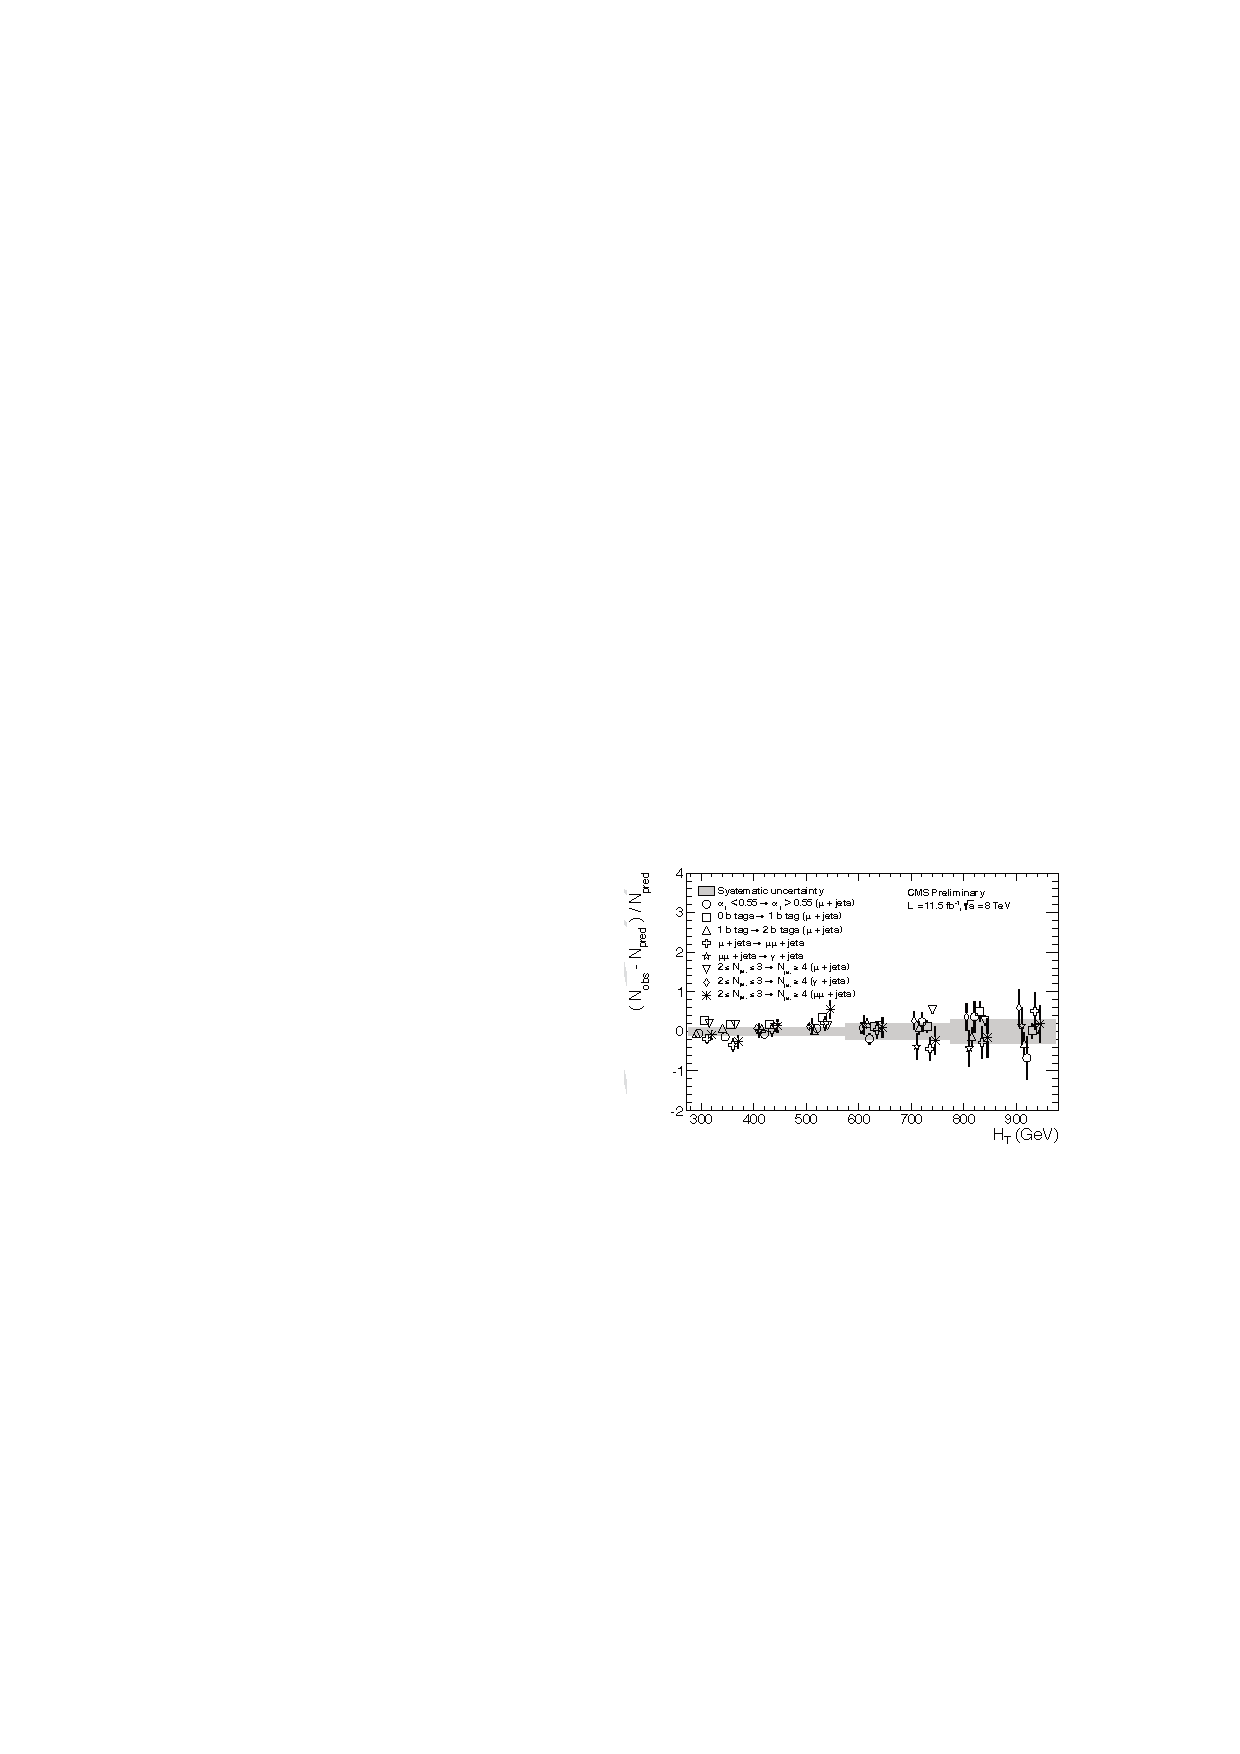
\includegraphics[width = 1.0\linewidth]{plots/syst-ge4j_varied.pdf}
\centering
(b) 
\end{minipage}
\caption[Sets of closure tests overlaid on top of the systematic uncertainty used for each of the five \theht regions.]{Sets of closure tests (open symbols) overlaid on top of the systematic uncertainty used for each of the five \theht regions (shaded bands) and for the two different jet multiplicity bins (a) $2 \leq n_{jet} \leq 3$ and (b) $n_{jet} \geq 4$.}
\label{fig:xsecvariedge4j}
\end{figure}

\def\arraystretch{1.3}
\begin{table}[ht!]
\begin{center}
\footnotesize
\begin{tabular}{ cccccc}
\hline\hline
\multicolumn{2}{c}{}               & \multicolumn{4}{c}{$H_{T}$ (GeV)} \\
$n_{b}^{reco}$ & Cross Section     & 275--325                  & 325--375                  & 375--475                  & 475--575                 \\ 
\hline
 0 & Nominal                       & 0.303  $\pm$  0.010       & 0.258  $\pm$  0.007       & 0.192  $\pm$  0.003       & 0.148  $\pm$  0.004      \\
 0 & Varied                        & 0.300  $\pm$  0.010       & 0.256  $\pm$  0.007       & 0.191  $\pm$  0.003       & 0.147  $\pm$  0.004      \\ 
 1 & Nominal                       & 0.294  $\pm$  0.005       & 0.246  $\pm$  0.004       & 0.189  $\pm$  0.003       & 0.139  $\pm$  0.003      \\
 1 & Varied                        & 0.295  $\pm$  0.006       & 0.248  $\pm$  0.004       & 0.191  $\pm$  0.003       & 0.140  $\pm$  0.003      \\ 
 2 & Nominal                       & 0.208  $\pm$  0.003       & 0.183  $\pm$  0.004       & 0.145  $\pm$  0.003       & 0.123  $\pm$  0.004      \\
 2 & Varied                        & 0.211  $\pm$  0.004       & 0.185  $\pm$  0.004       & 0.147  $\pm$  0.003       & 0.124  $\pm$  0.004      \\ 
 3 & Nominal                       & 0.214  $\pm$  0.005       & 0.202  $\pm$  0.007       & 0.159  $\pm$  0.006       & 0.140  $\pm$  0.007      \\
 3 & Varied                        & 0.215  $\pm$  0.005       & 0.203  $\pm$  0.007       & 0.159  $\pm$  0.006       & 0.140  $\pm$  0.007      \\ 
 $\geq$4 & Nominal                 & 0.220  $\pm$  0.015       & 0.245  $\pm$  0.035       & 0.119  $\pm$  0.009       & -                         \\
 $\geq$4 & Varied                  & 0.220  $\pm$  0.015       & 0.245  $\pm$  0.035       & 0.119  $\pm$  0.009       & -                          \\  
\hline\hline
$n_{b}^{reco}$ & Cross Section   & 575--675                  & 675--775                  & 775--875                  & 875--$\infty$            \\ 
\hline
0 & Nominal                        & 0.119  $\pm$  0.004       & 0.098  $\pm$  0.005       & 0.077  $\pm$  0.006       & 0.049  $\pm$  0.005      \\
0 & Varied                         & 0.120  $\pm$  0.005       & 0.098  $\pm$  0.006       & 0.077  $\pm$  0.007       & 0.049  $\pm$  0.005      \\ 
1 & Nominal                        & 0.115  $\pm$  0.004       & 0.093  $\pm$  0.005       & 0.075  $\pm$  0.007       & 0.063  $\pm$  0.006      \\
1 & Varied                         & 0.116  $\pm$  0.004       & 0.098  $\pm$  0.005       & 0.081  $\pm$  0.007       & 0.065  $\pm$  0.006      \\ 
2 & Nominal                        & 0.096  $\pm$  0.005       & 0.070  $\pm$  0.006       & 0.051  $\pm$  0.007       & 0.063  $\pm$  0.008      \\
2 & Varied                         & 0.098  $\pm$  0.005       & 0.073  $\pm$  0.006       & 0.053  $\pm$  0.007       & 0.064  $\pm$  0.008      \\ 
3 & Nominal                        & 0.114  $\pm$  0.009       & 0.065  $\pm$  0.007       & 0.070  $\pm$  0.017       & 0.092  $\pm$  0.020      \\
3 & Varied                         & 0.114  $\pm$  0.009       & 0.066  $\pm$  0.007       & 0.070  $\pm$  0.016       & 0.093  $\pm$  0.020      \\ 
\end{tabular}
\end{center}
\caption[Translation factors constructed from the \mupjets control sample and signal selction MC, to predict yields for the W + jets and \ttbar back-grounds in the signal region.]{Translation factors constructed from the \mupjets control sample and signal selction MC, to predict yields for the W + jets and \ttbar back-grounds in the signal region with (a) NNLO cross sections corrected by k-factors determined from a data sideband see Section (\ref{subsec:mckfactors}), marked as �Nominal�, and (b) the same cross sections but with those for W + jets and \ttbar varied up and down by 20\%, respectively, marked as �Varied�. No requirement is placed on the jet multiplicity of events within this table.}\label{tab:xsecvaried}
\end{table}
\def\arraystretch{1.0}


\chapter{Additional Material  For B-tag Template Method}
\label{app:templatematerial}
\section{Templates Fits in Simulation}
\label{app:templatemc}

Template fits for the three \ac{CSV} working points in the $n_{jet} = 3$, \theht $>$ 375 category:

\begin{figure}[ht]
\centering
\begin{minipage}[b]{0.51 \linewidth}
\vspace{30mm}
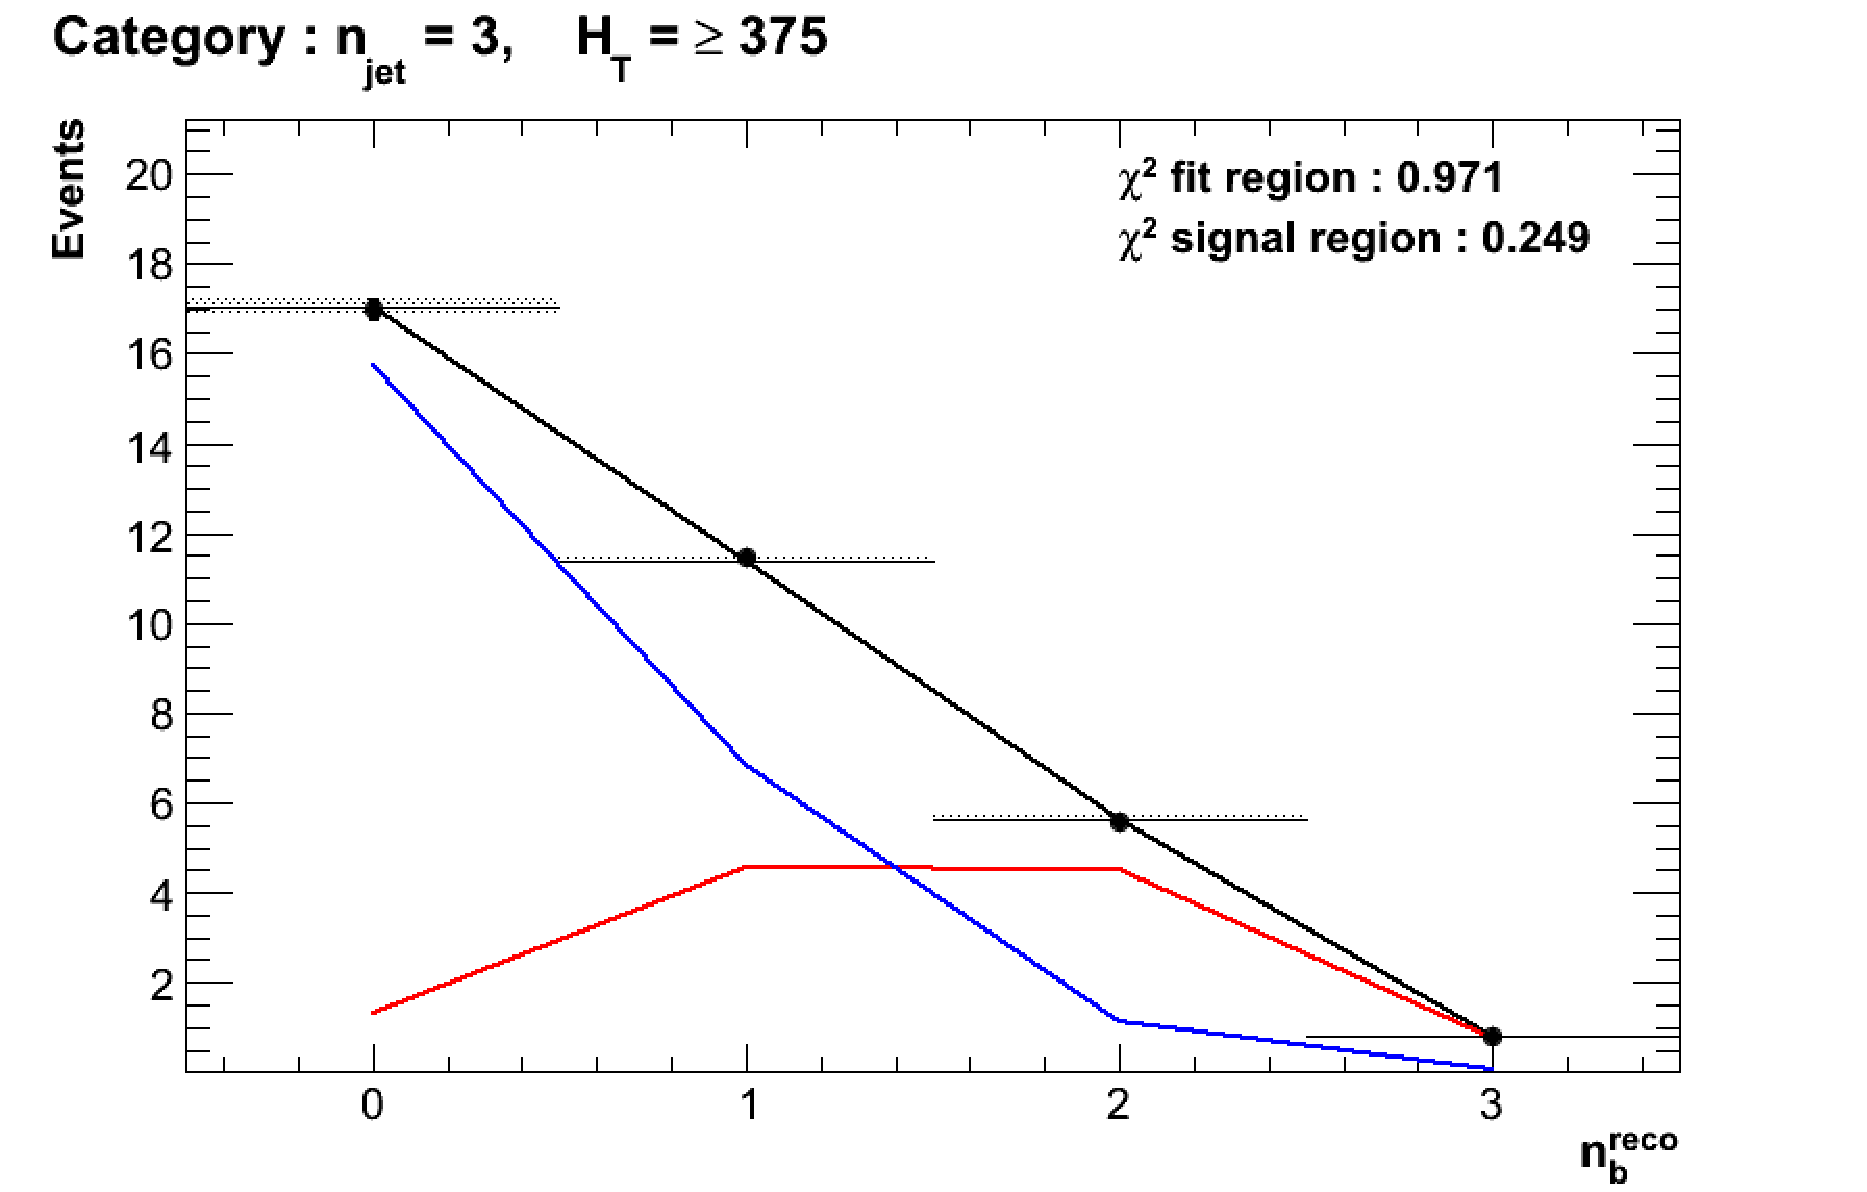
\includegraphics[width = 1.0\linewidth]{plots/ThesisPlots/Final_Fit_To_MC_Normal_Loose_HTBin_OneMuon_Template_375_jet_mult_3.pdf}
\centering (a) Loose working point $n_{jet}$ = 3 
\end{minipage}
\end{figure}
\begin{figure}
\begin{minipage}[b]{0.51\linewidth}
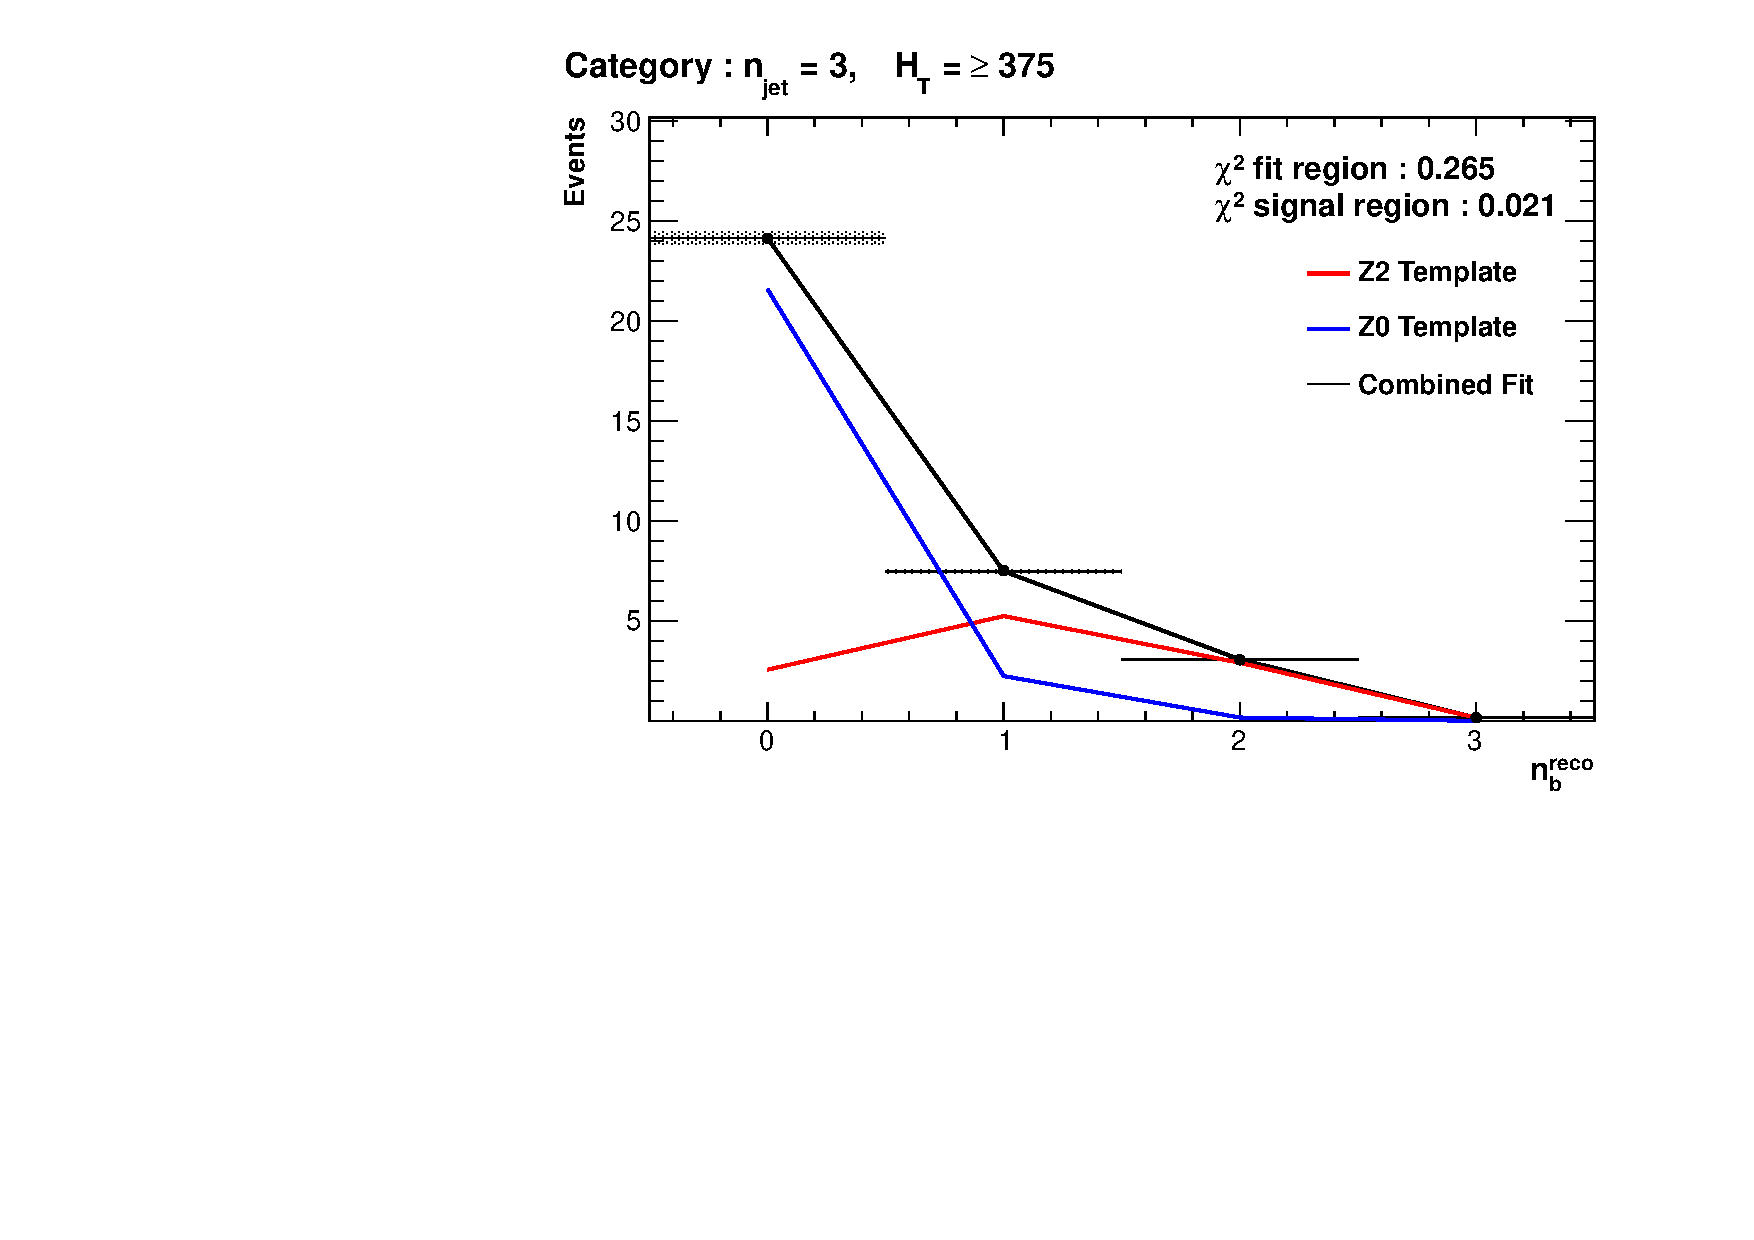
\includegraphics[width = 1.0\linewidth]{plots/ThesisPlots/Final_Fit_To_MC_Normal_Medium_HTBin_OneMuon_Template_375_jet_mult_3.pdf}
\centering (b) Medium working point $n_{jet}$ = 3 
\end{minipage}
\quad
\begin{minipage}[b]{0.51\linewidth}
\centering
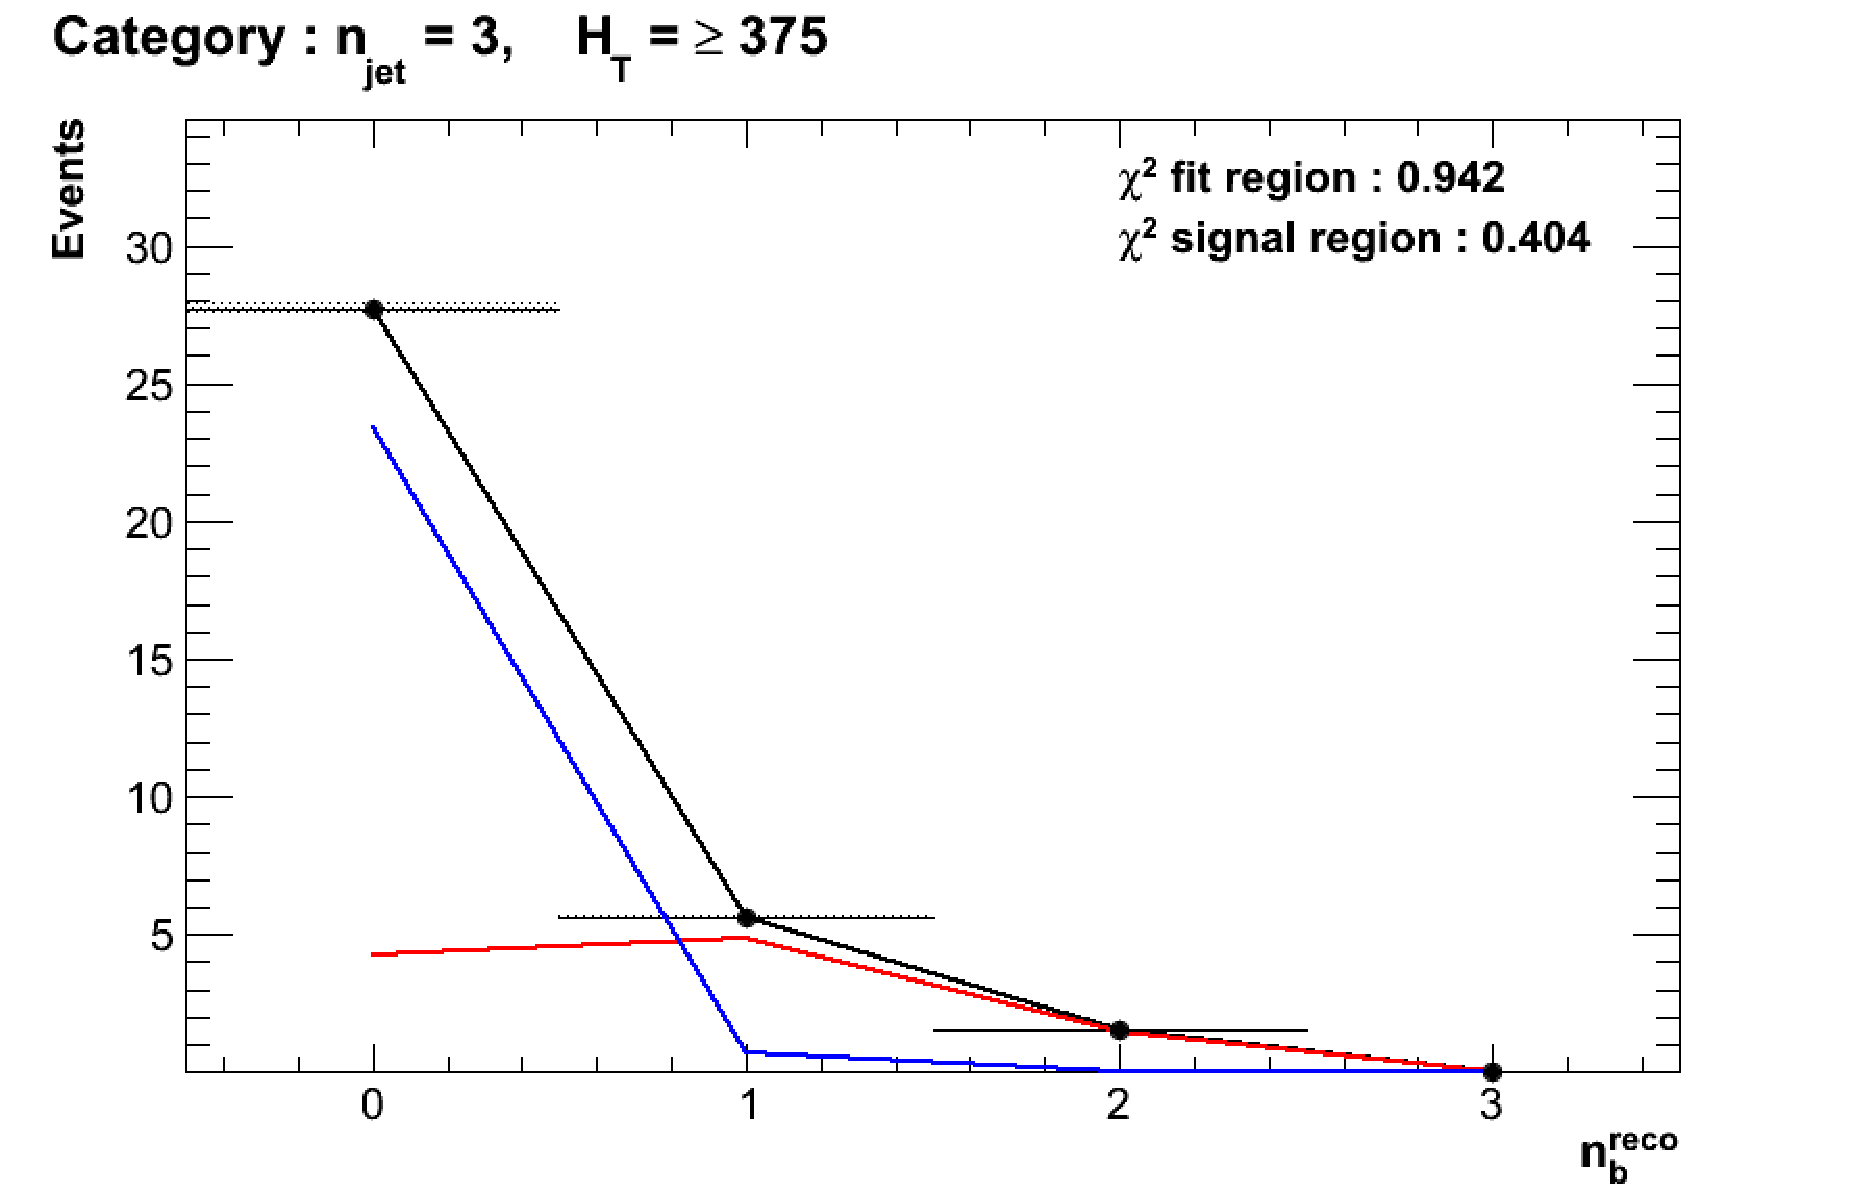
\includegraphics[width = 1.0\linewidth]{plots/ThesisPlots/Final_Fit_To_MC_Normal_Tight_HTBin_OneMuon_Template_375_jet_mult_3.pdf}
\centering (c) Tight working point $n_{jet} =$ 3 
\end{minipage}
\caption[The results of fitting the Z = 0 and Z = 2 templates to the $n_{b}^{reco}$ = 0, 1, 2 bins taken directly from simulation in the region \theht $>$ 375 \GeV, for the $n_{jet} = 3$ category.]{The results of fitting the Z = 0 and Z = 2 templates to the $n_{b}^{reco}$ = 0, 1, 2 bins taken directly from simulation in the region \theht $>$ 375 \GeV, for the $n_{jet} = 3$ category. The blue template represents Z = 0, while the red template represents Z = 2. Grey bands represent the statistical uncertainty of the fit.The $\chi^{2}$ parameter displayed represents the goodness of fit to the low$ n_{b}^{reco}$ (0-2) control region.}
\label{app:template_closure_njet3}
\end{figure}

\FloatBarrier

Template fits for the three \ac{CSV} working points in the $n_{jet} = 4$, \theht $>$ 375 category:

\begin{figure}[ht]
\centering
\begin{minipage}[b]{0.51\linewidth}
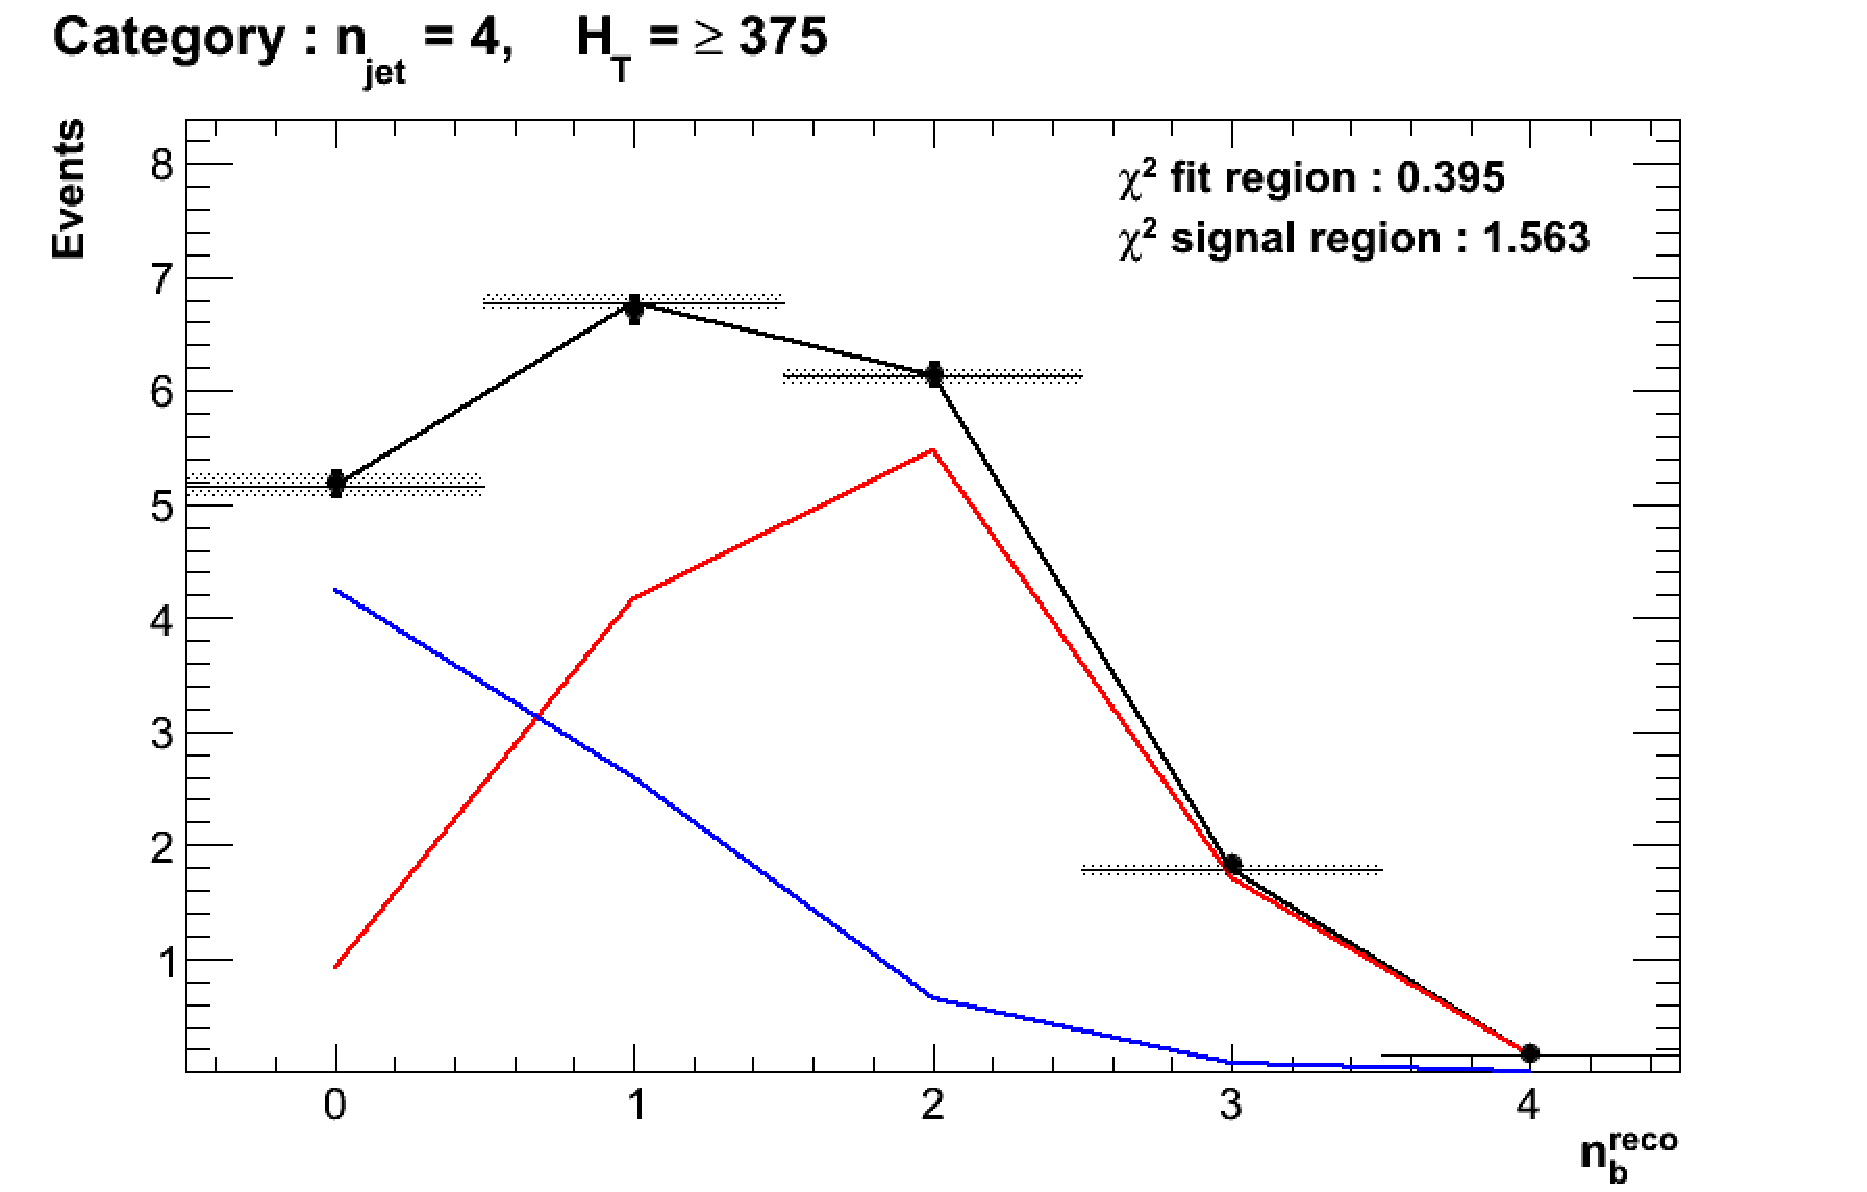
\includegraphics[width = 1.0\linewidth]{plots/ThesisPlots/Final_Fit_To_MC_Normal_Loose_HTBin_OneMuon_Template_375_jet_mult_4.pdf}
\centering (a) Loose working point $n_{jet}$ = 4 
\end{minipage}
\quad
\begin{minipage}[b]{0.51\linewidth}
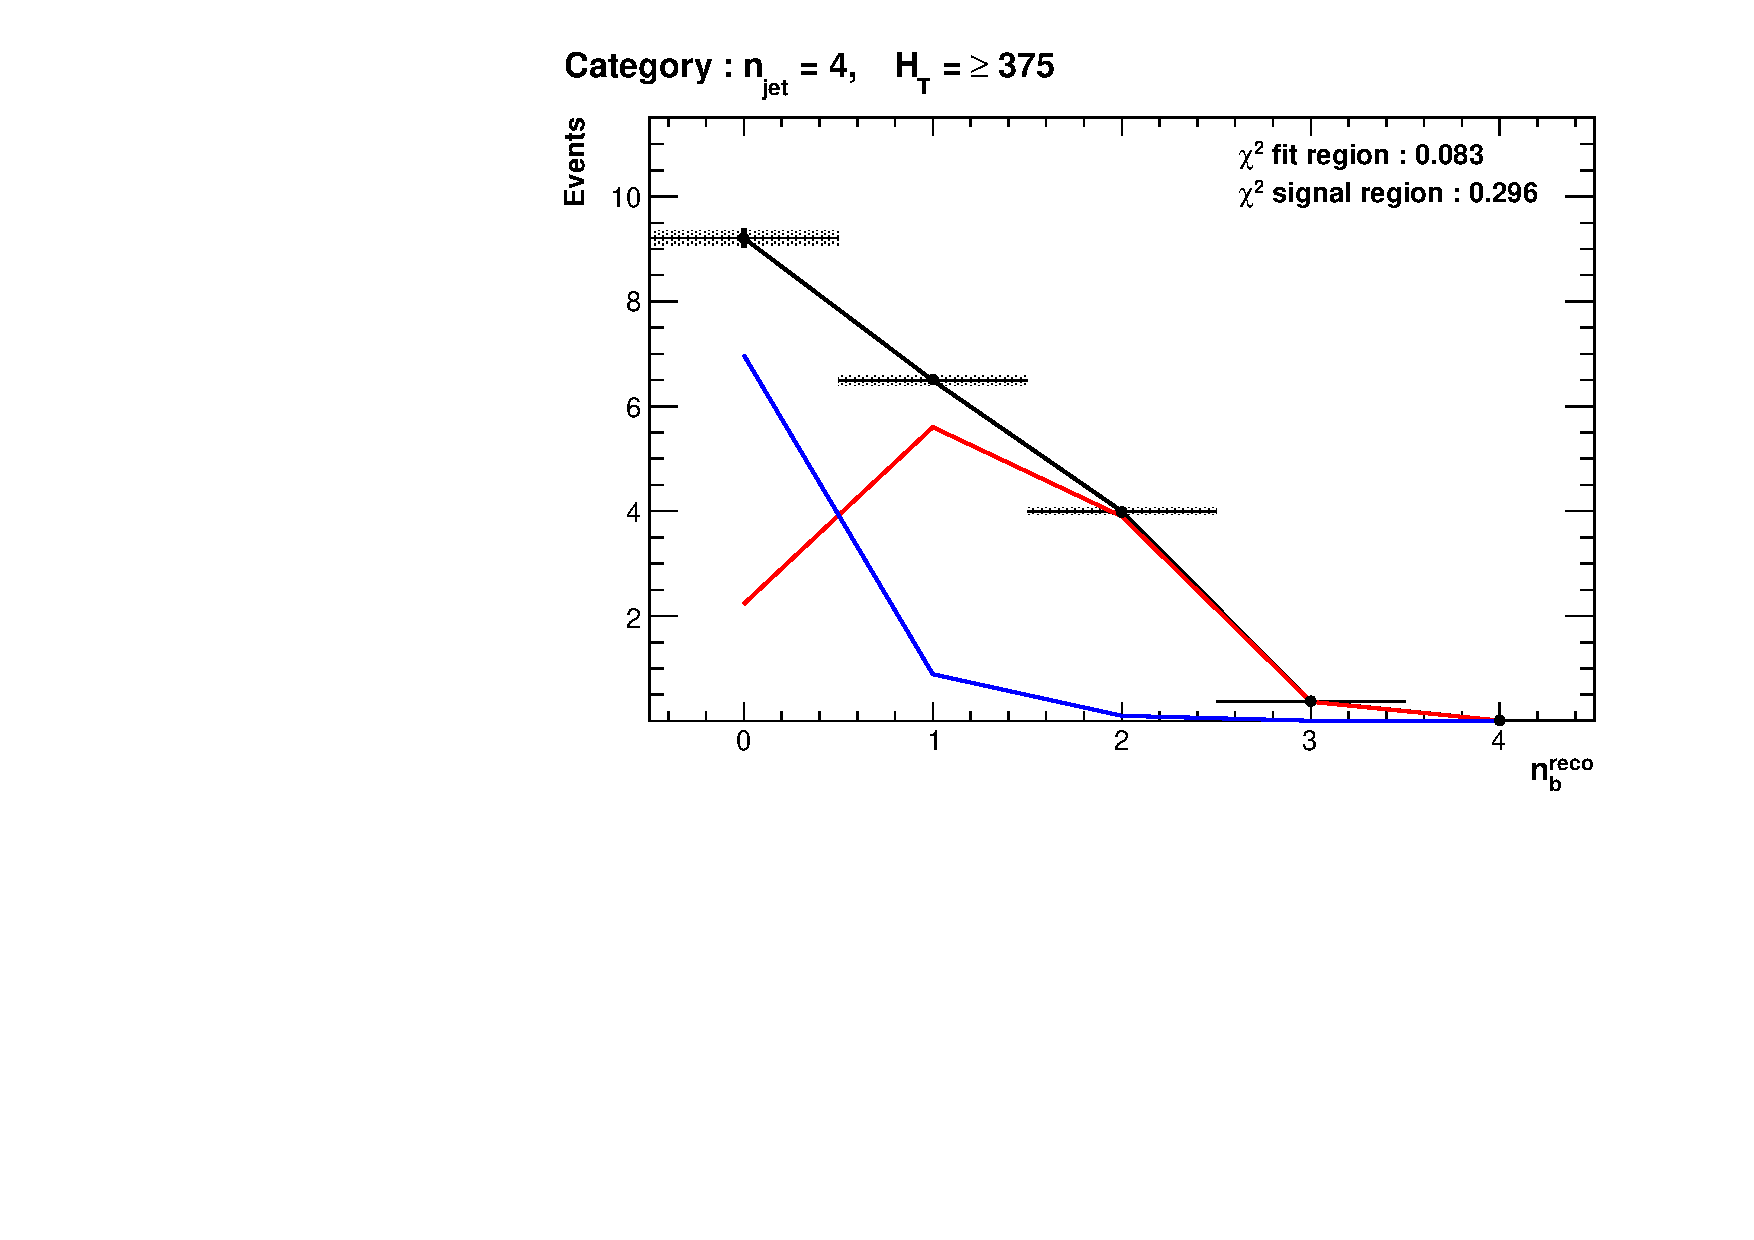
\includegraphics[width = 1.0\linewidth]{plots/ThesisPlots/Final_Fit_To_MC_Normal_Medium_HTBin_OneMuon_Template_375_jet_mult_4.pdf}
\centering (b) Medium working point $n_{jet}$ = 4 
\end{minipage}
\quad
\begin{minipage}[b]{0.51\linewidth}
\centering
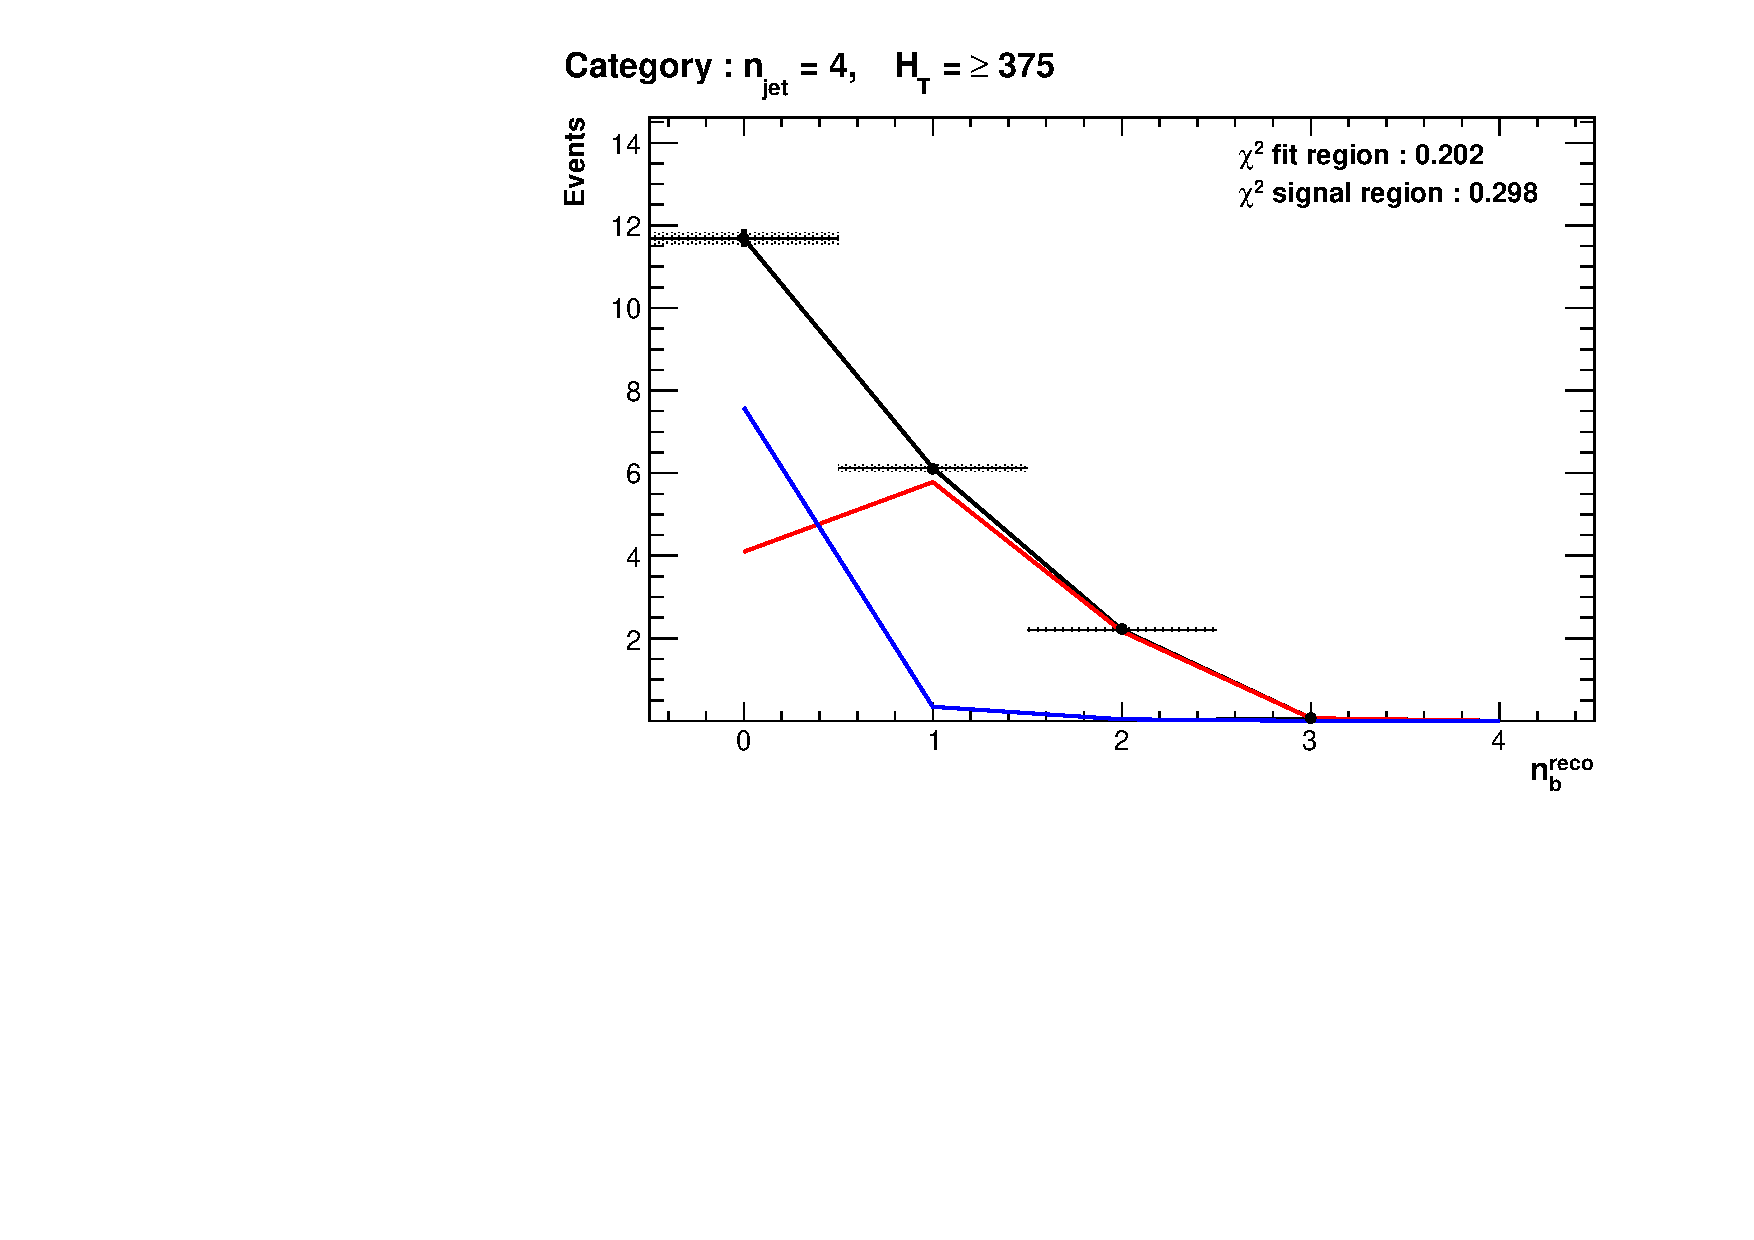
\includegraphics[width = 1.0\linewidth]{plots/ThesisPlots/Final_Fit_To_MC_Normal_Tight_HTBin_OneMuon_Template_375_jet_mult_4.pdf}
\centering (c) Tight working point $n_{jet} =$ 4 
\end{minipage}
\caption[The results of fitting the Z = 0 and Z = 2 templates to the $n_{b}^{reco}$ = 0, 1, 2 bins taken directly from simulation in the region \theht $>$ 375 \GeV, for the $n_{jet} = 4$ category.]{The results of fitting the Z = 0 and Z = 2 templates to the $n_{b}^{reco}$ = 0, 1, 2 bins taken directly from simulation in the region \theht $>$ 375 \GeV,  for the $n_{jet} = 4$ category. The blue template represents Z = 0, while the red template represents Z = 2. Grey bands represent the statistical uncertainty of the fit.The $\chi^{2}$ parameter displayed represents the goodness of fit to the low$ n_{b}^{reco}$ (0-2) control region.}
\label{fig:template_closure_high}
\end{figure}

\FloatBarrier

\section{Pull Distributions for Template Fits}
\label{app:templatepulldistributions}

\begin{figure}[ht]
\centering
\begin{minipage}[b]{0.48 \linewidth}
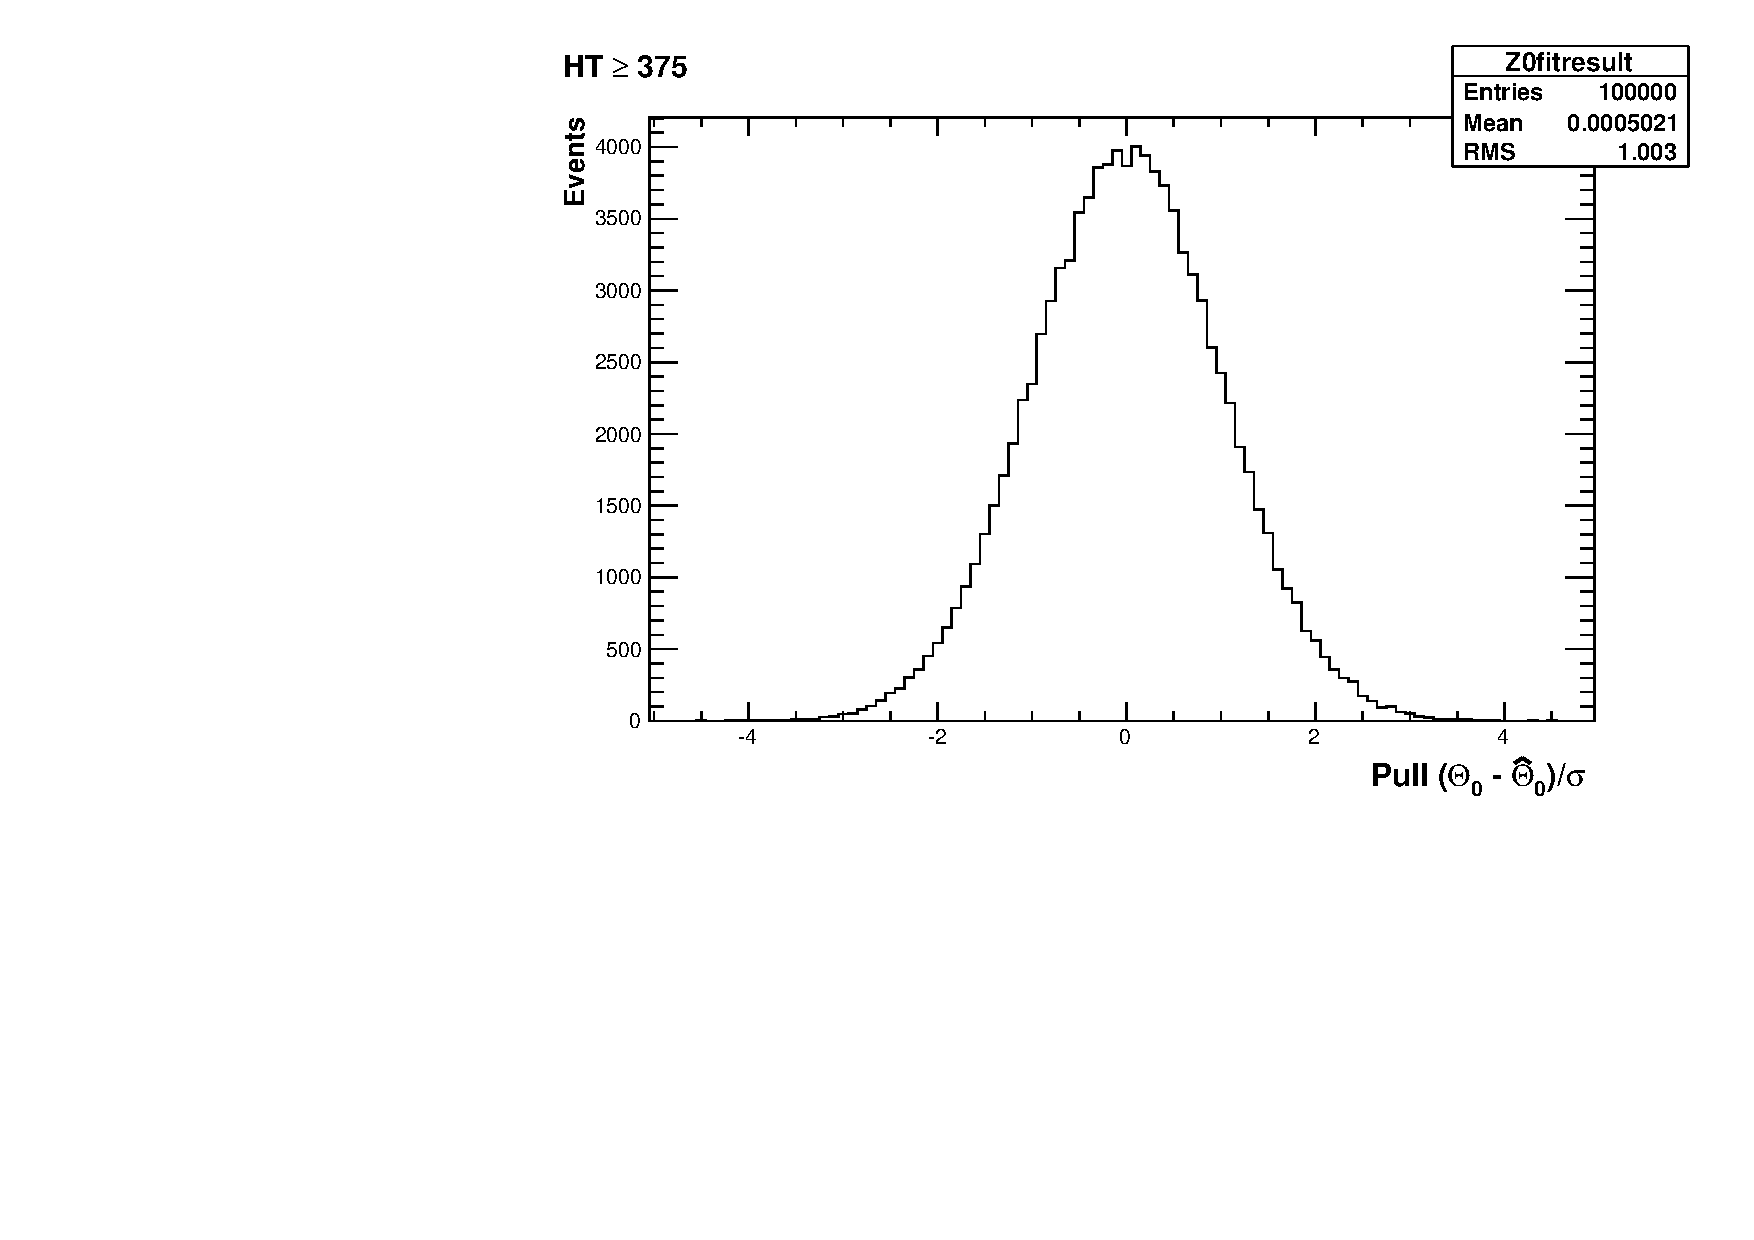
\includegraphics[width = 1.0\linewidth]{plots/ThesisPlots/Pull_Plot_Z0_HTbin_Template_375_jet_mult_3_num_param_3.pdf}
\centering (a) Z0 Template, \theht $> 375$ ,  $n_{jet} = 3$
\end{minipage}
\quad
\begin{minipage}[b]{0.48\linewidth}
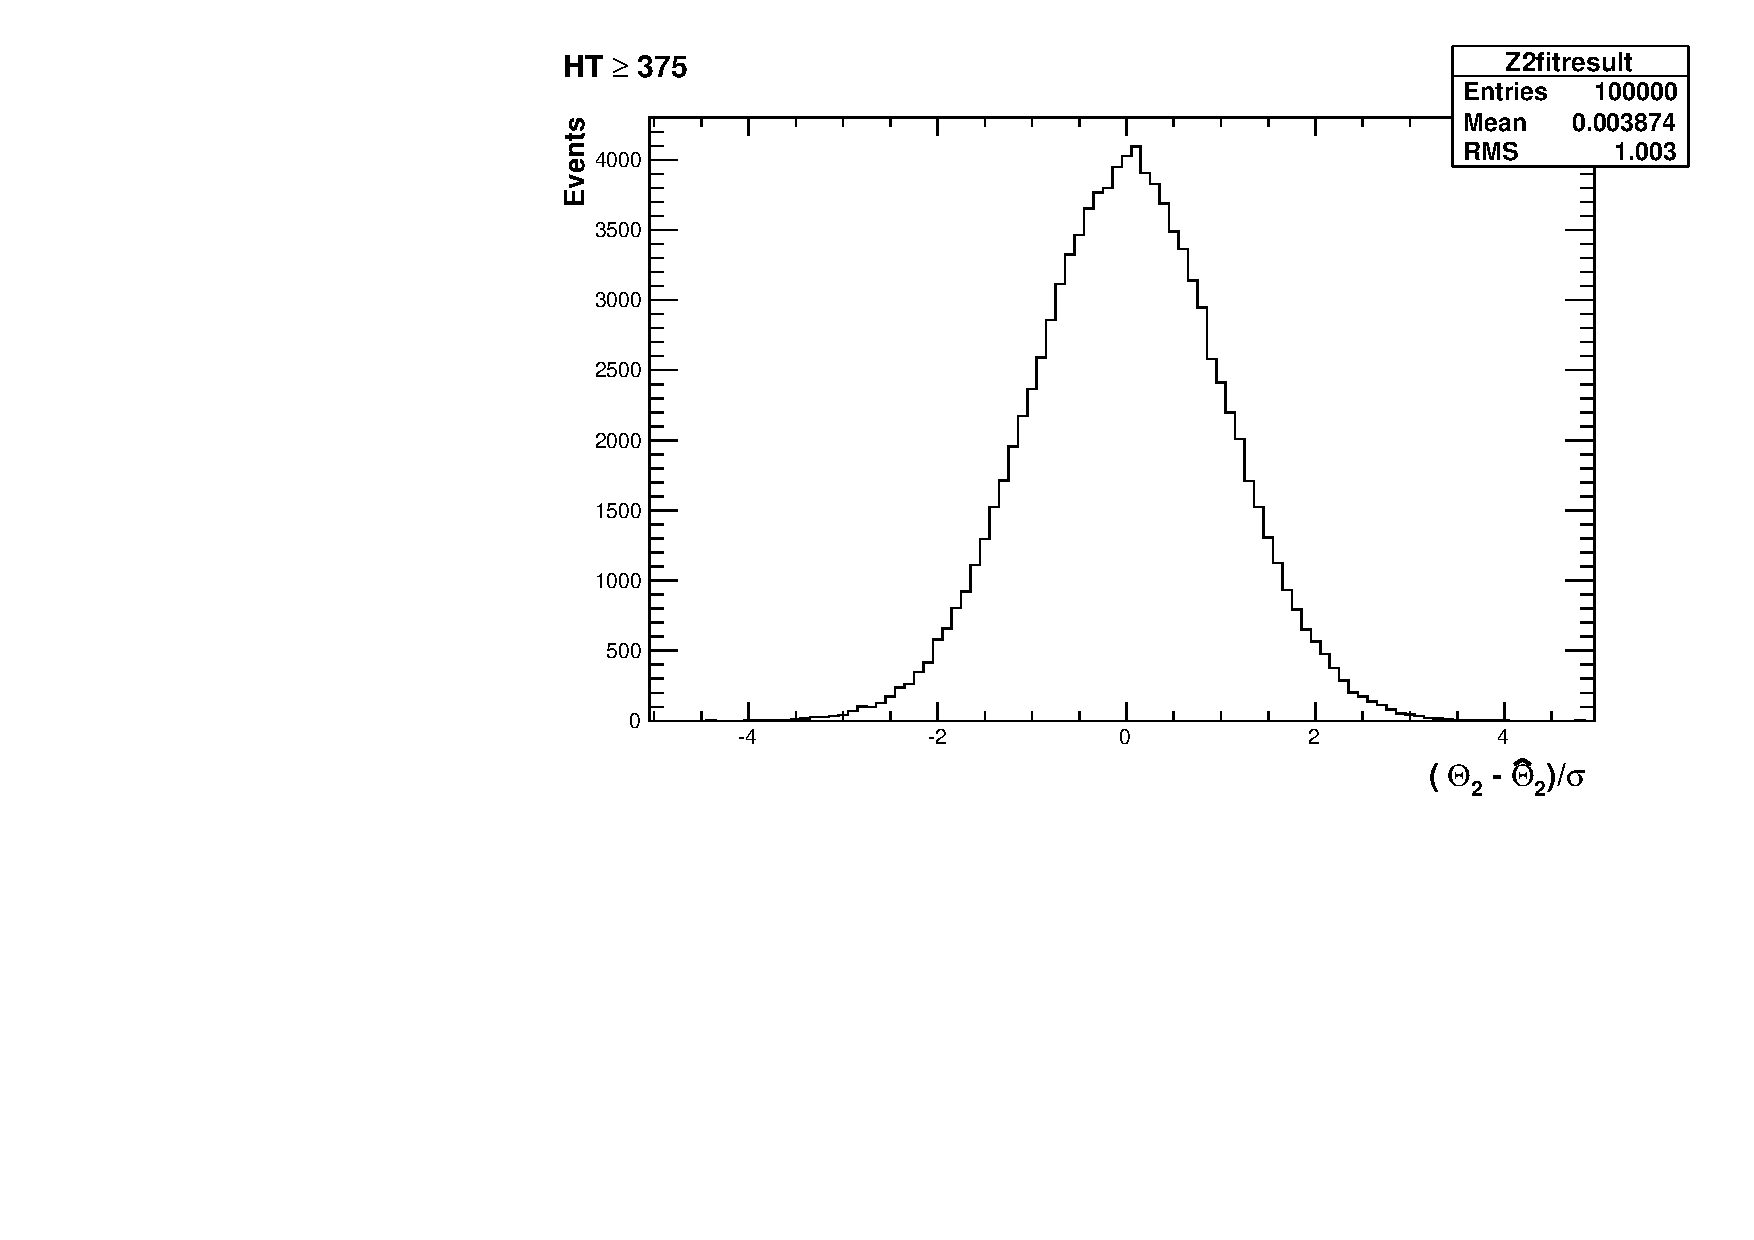
\includegraphics[width = 1.0\linewidth]{plots/ThesisPlots/Pull_Plot_Z2_HTbin_Template_375_jet_mult_3_num_param_3.pdf}
\centering (b) Z2 Template, \theht $> 375$ ,  $n_{jet} = 3$
\end{minipage}
\quad
\begin{minipage}[b]{0.48 \linewidth}
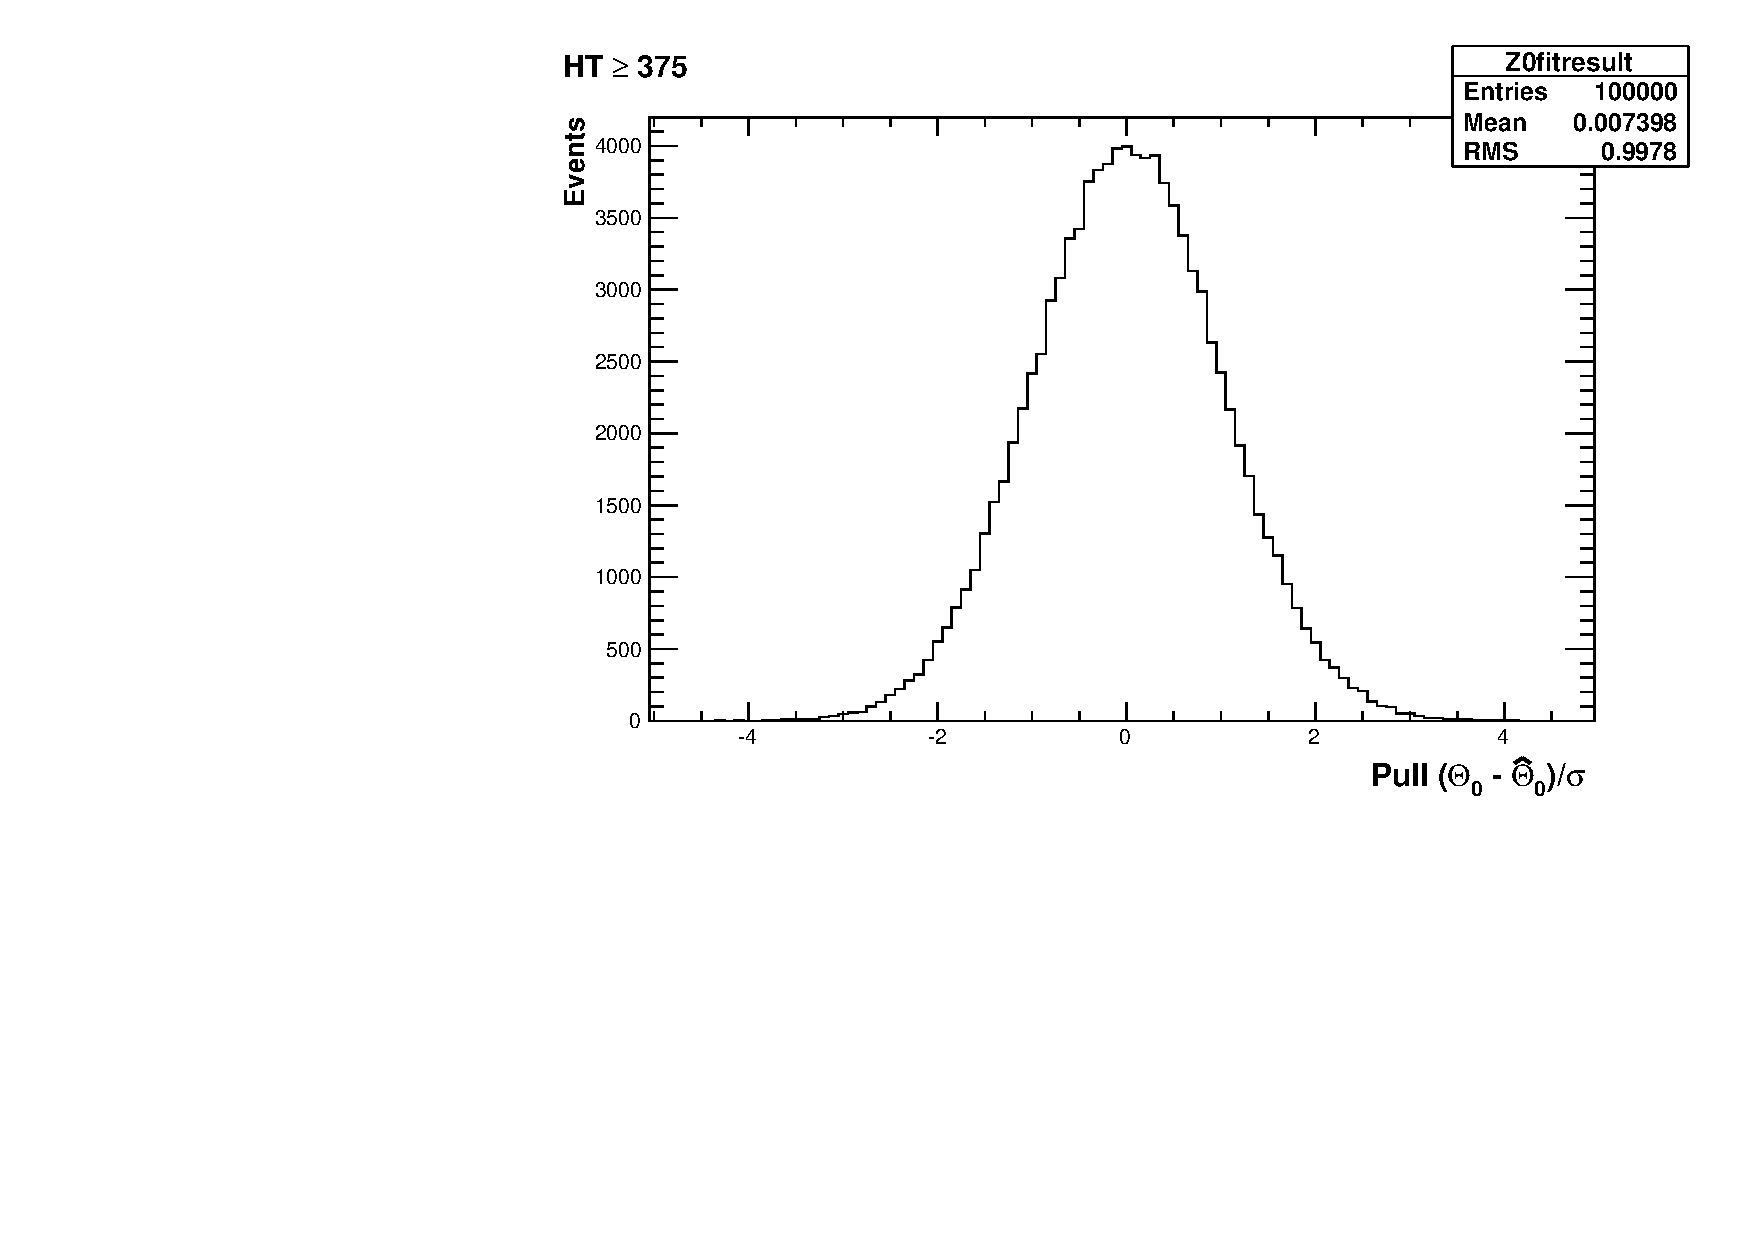
\includegraphics[width = 1.0\linewidth]{plots/ThesisPlots/Pull_Plot_Z0_HTbin_Template_375_jet_mult_4_num_param_3.pdf}
\centering (a) Z0 Template, \theht $> 375$ ,  $n_{jet} = 4$
\end{minipage}
\quad
\begin{minipage}[b]{0.48\linewidth}
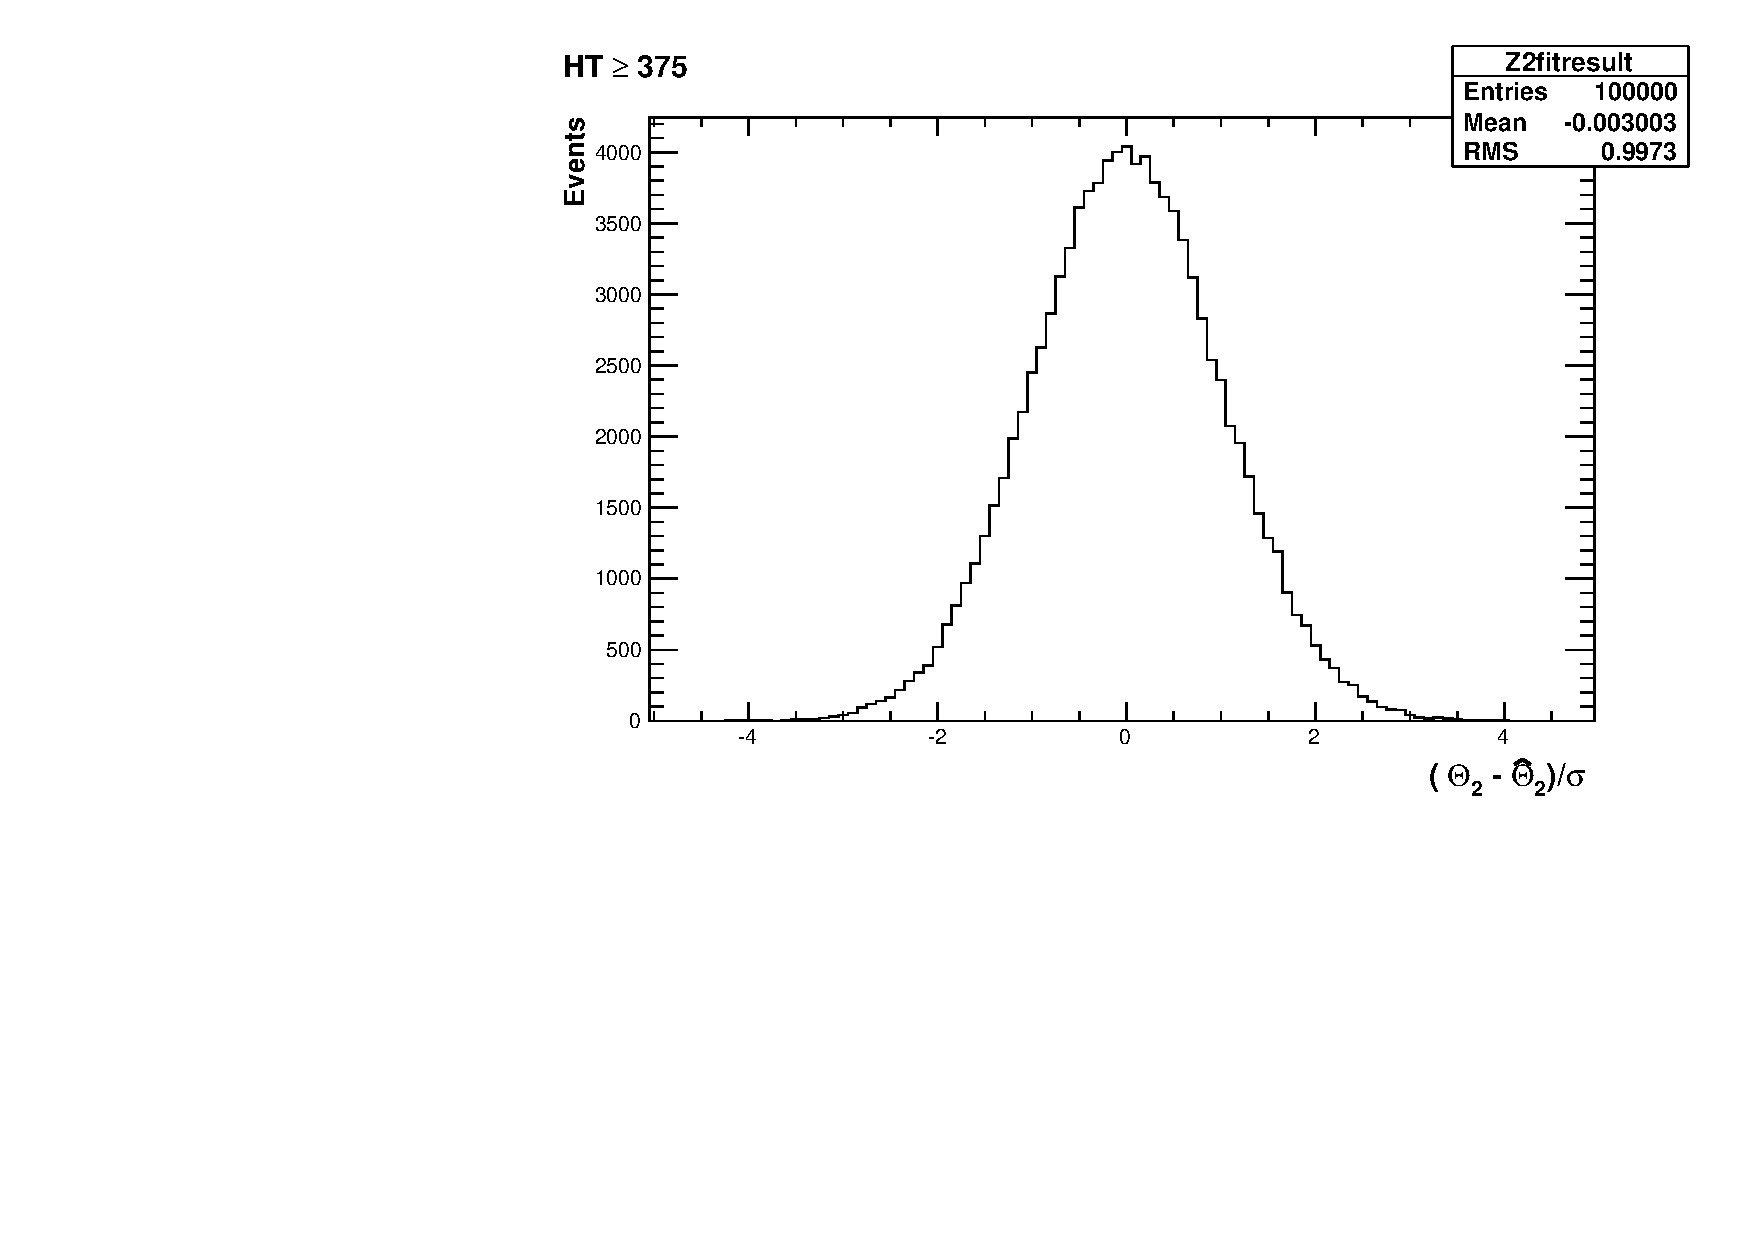
\includegraphics[width = 1.0\linewidth]{plots/ThesisPlots/Pull_Plot_Z2_HTbin_Template_375_jet_mult_4_num_param_3.pdf}
\centering (b) Z2 Template, \theht $> 375$ ,  $n_{jet} = 4$
\end{minipage}
\quad
\begin{minipage}[b]{0.48 \linewidth}
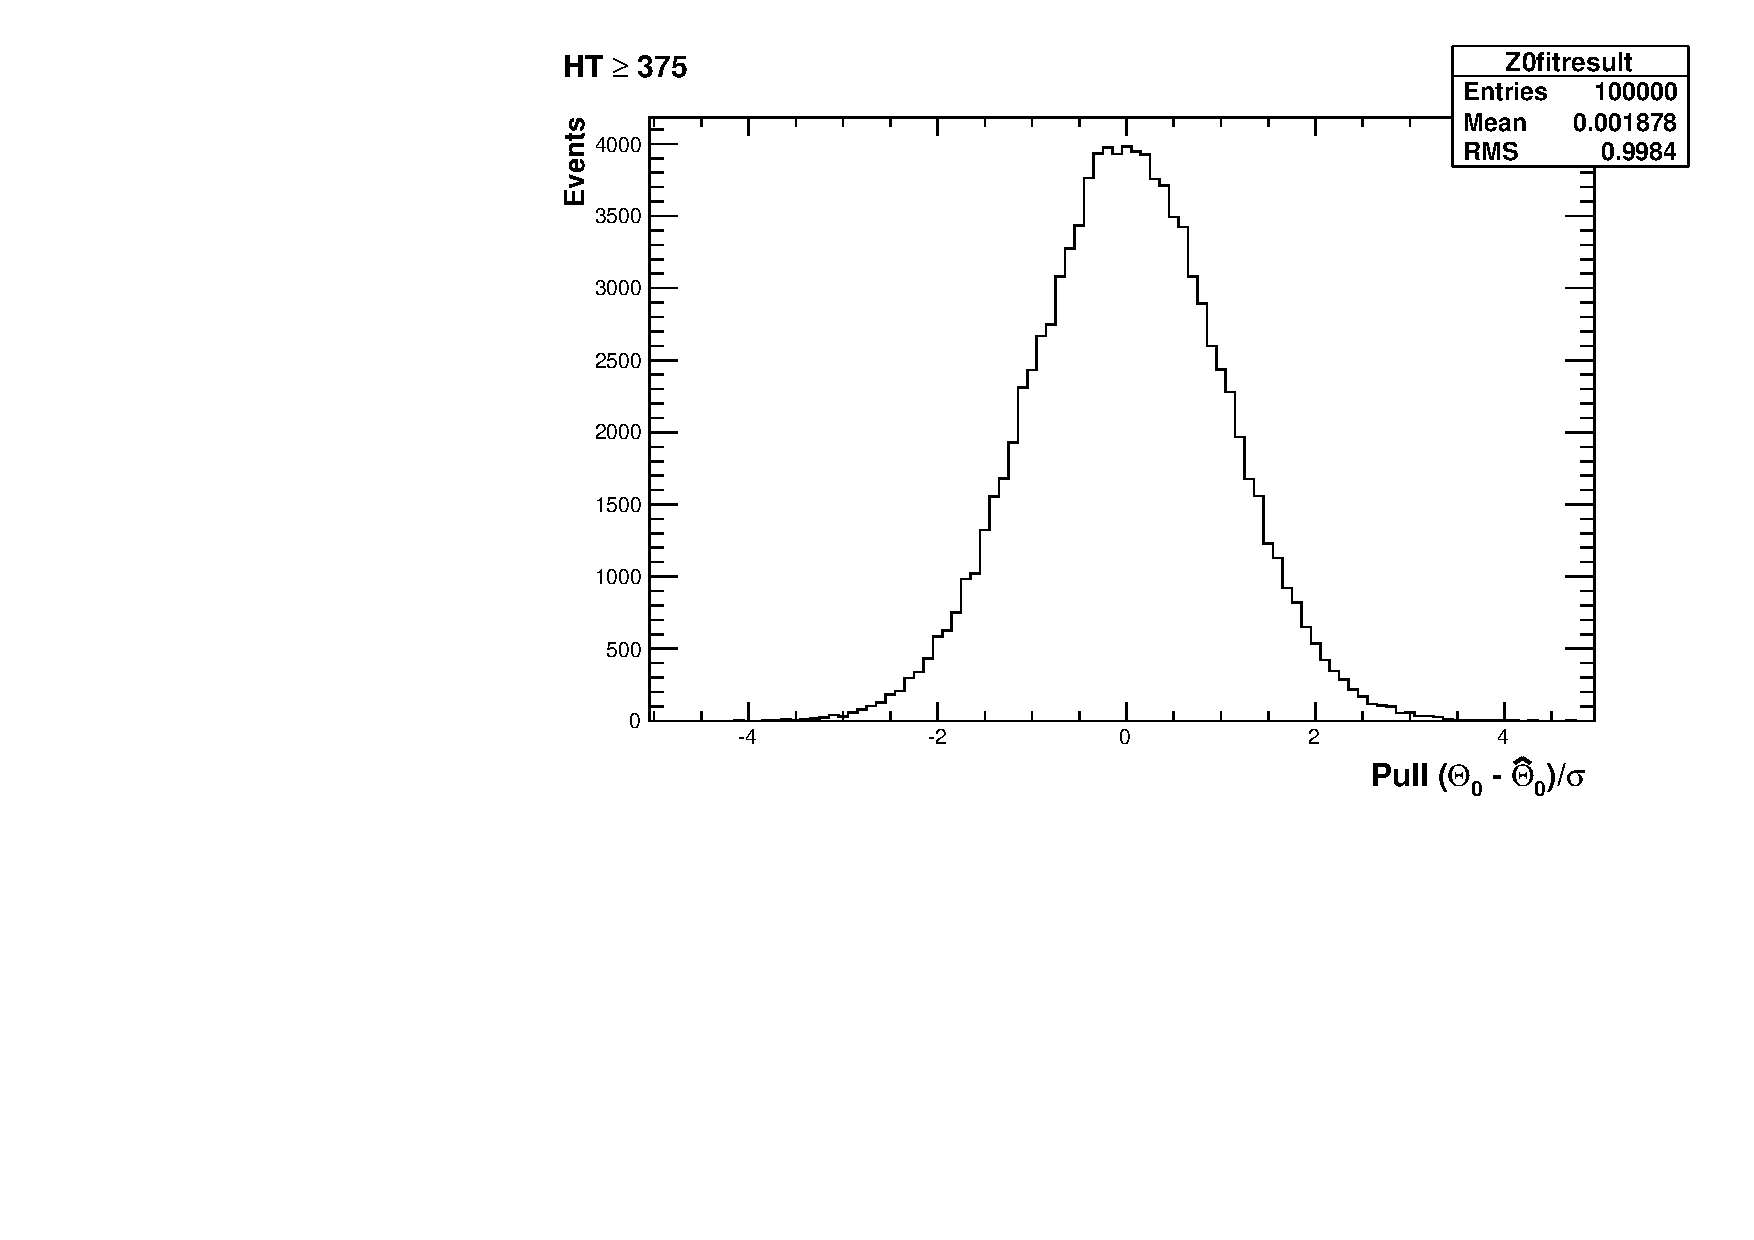
\includegraphics[width = 1.0\linewidth]{plots/ThesisPlots/Pull_Plot_Z0_HTbin_Template_375_jet_mult_5_num_param_3.pdf}
\centering (a) Z0 Template, \theht $> 375$ ,  $n_{jet} \geq 5$
\end{minipage}
\quad
\begin{minipage}[b]{0.48\linewidth}
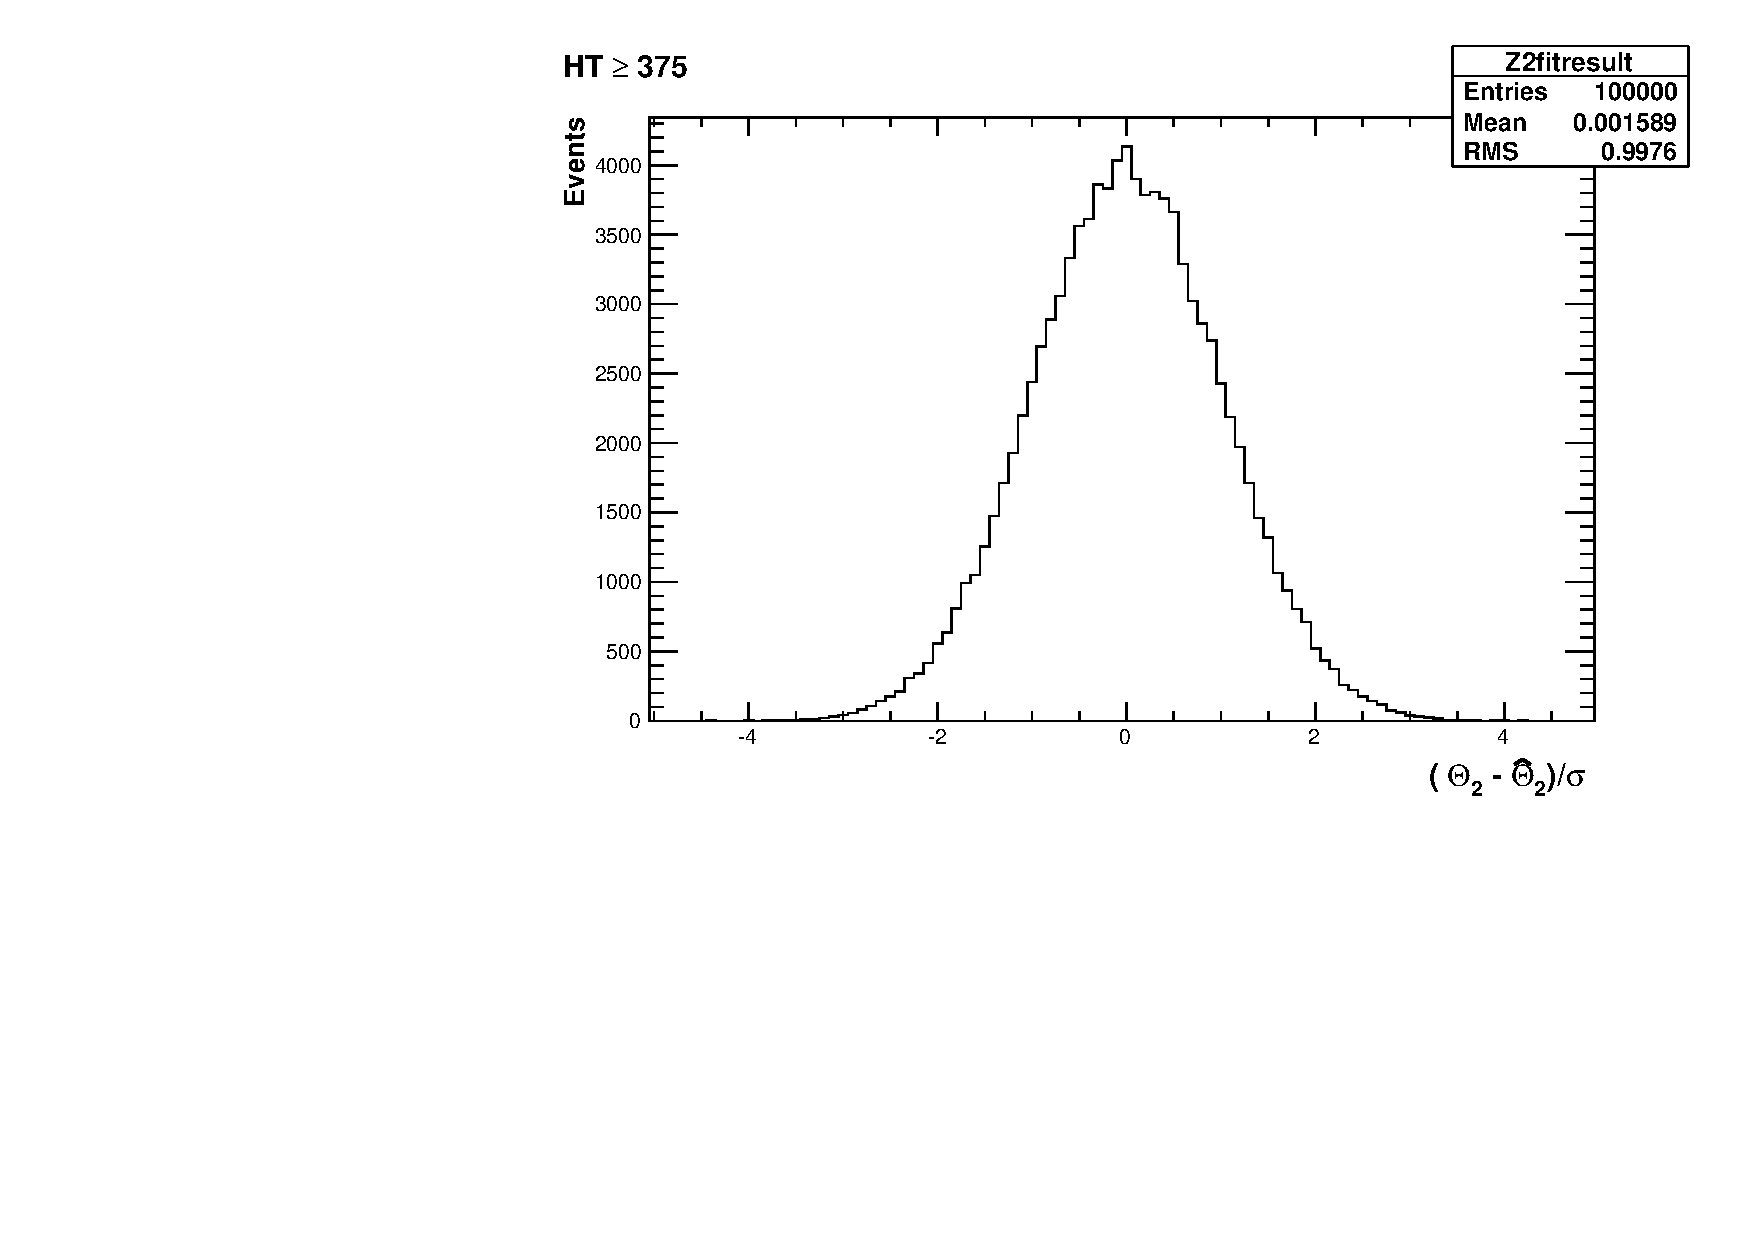
\includegraphics[width = 1.0\linewidth]{plots/ThesisPlots/Pull_Plot_Z2_HTbin_Template_375_jet_mult_5_num_param_3.pdf}
\centering (b) Z2 Template, \theht $> 375$ ,  $n_{jet} \geq 5$
\end{minipage}
\caption[Pull distributions of $\frac{(\theta - \hat{\theta})}{\sigma}$for $10^{4}$ pseudo-experiments generated from a gaussian distribution centred on the $n_{b}^{reco}$ template values from simulation with width $\sigma$.]{Pull distributions of $\frac{(\theta - \hat{\theta})}{\sigma}$for $10^{4}$ pseudo-experiments generated from a gaussian distribution centred on the $n_{b}^{reco}$ template values from simulation with width $\sigma$. Distributions are shown for both Z0 and Z2 templates for the medium \ac{CSV} working point.}
\label{app:templatepulldistributionsmedium}
\end{figure}



\section{Templates Fits in Data Control Sample}
\label{app:templatedata}

Template fits for the three \theht bins, in the $n_{jet} = 3$,  medium \ac{CSV} working point:

\begin{figure}[ht]
\centering
\begin{minipage}[b]{0.51 \linewidth}
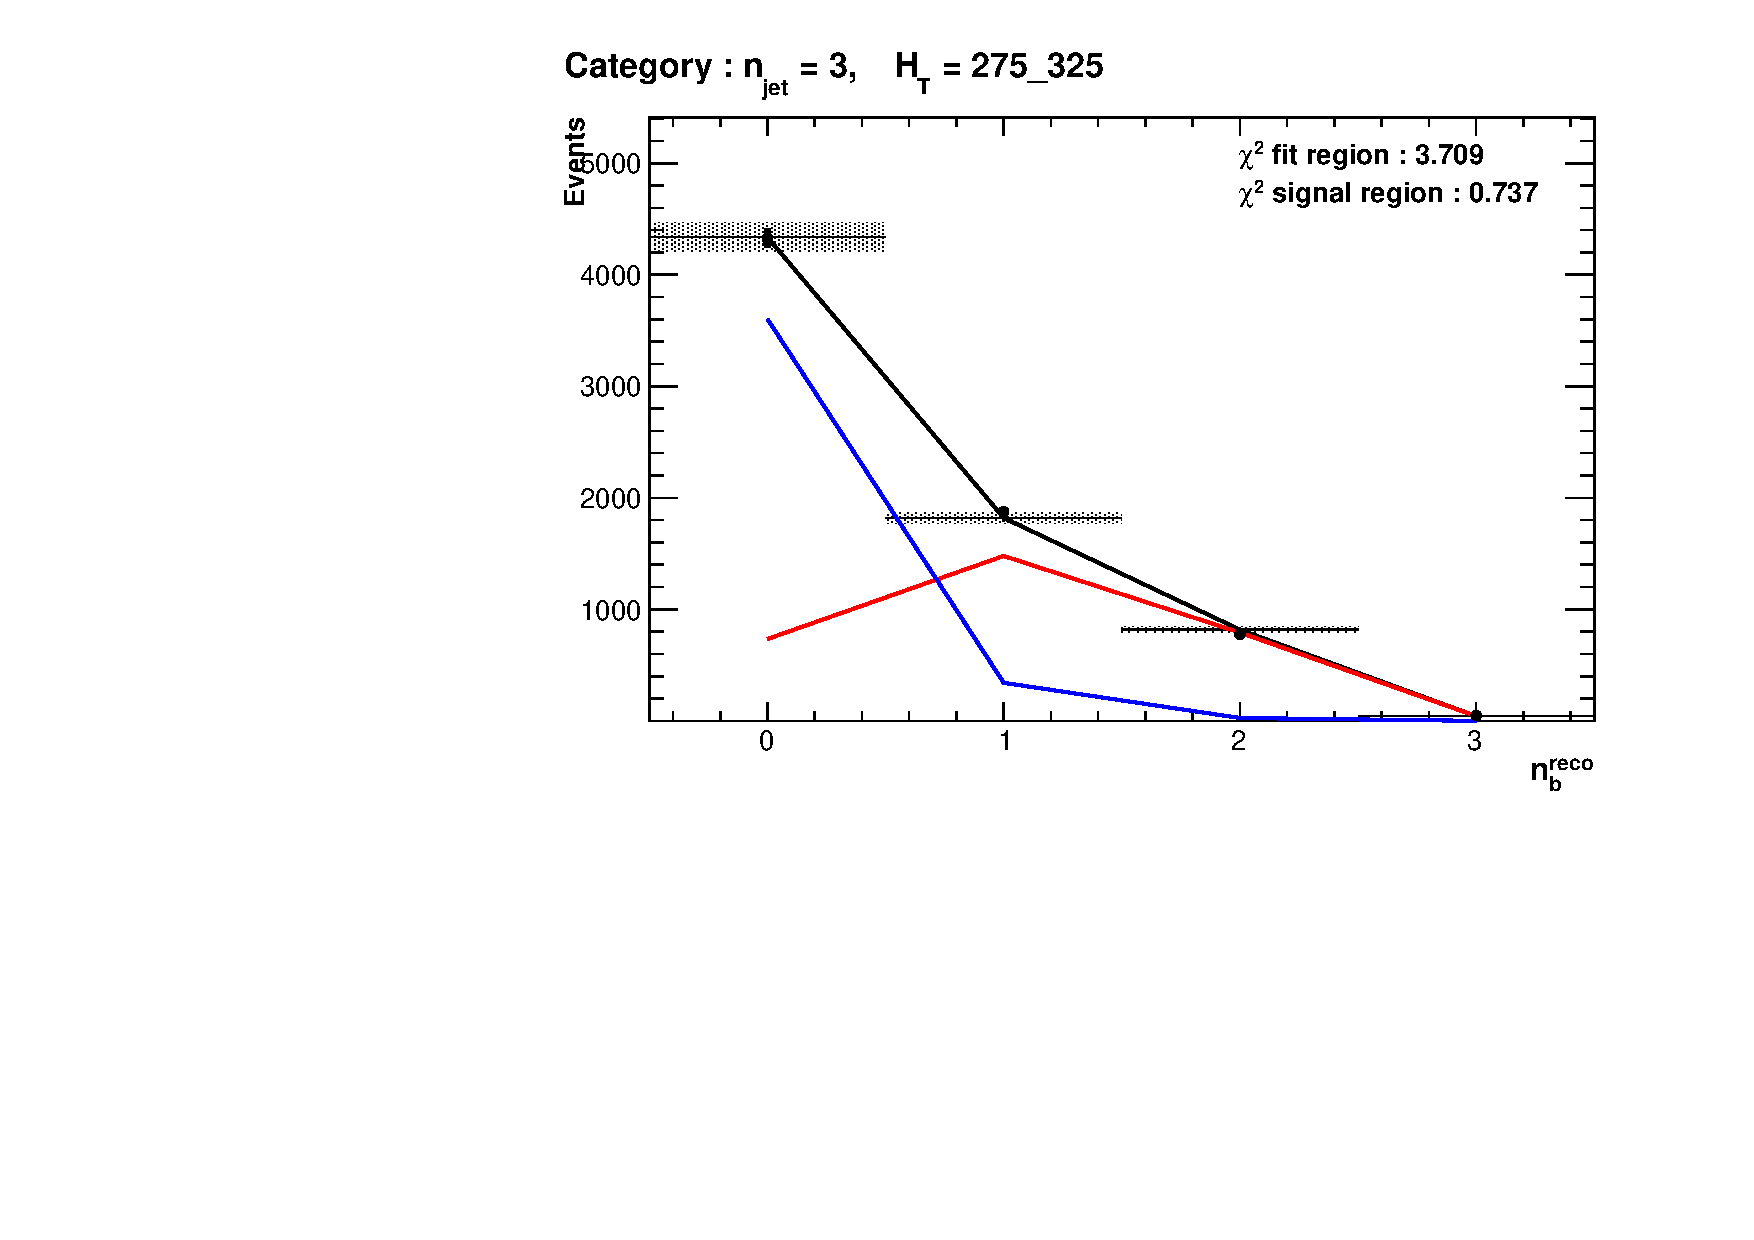
\includegraphics[width = 1.0\linewidth]{plots/ThesisPlots/Final_Fit_To_Data_Normal_Medium_HTBin_OneMuon_275_325_jet_mult_3.pdf}
\centering (a) $n_{jet} =$  3 , 275 $<$ \theht $<$ 325
\end{minipage}
\quad
\begin{minipage}[b]{0.51\linewidth}
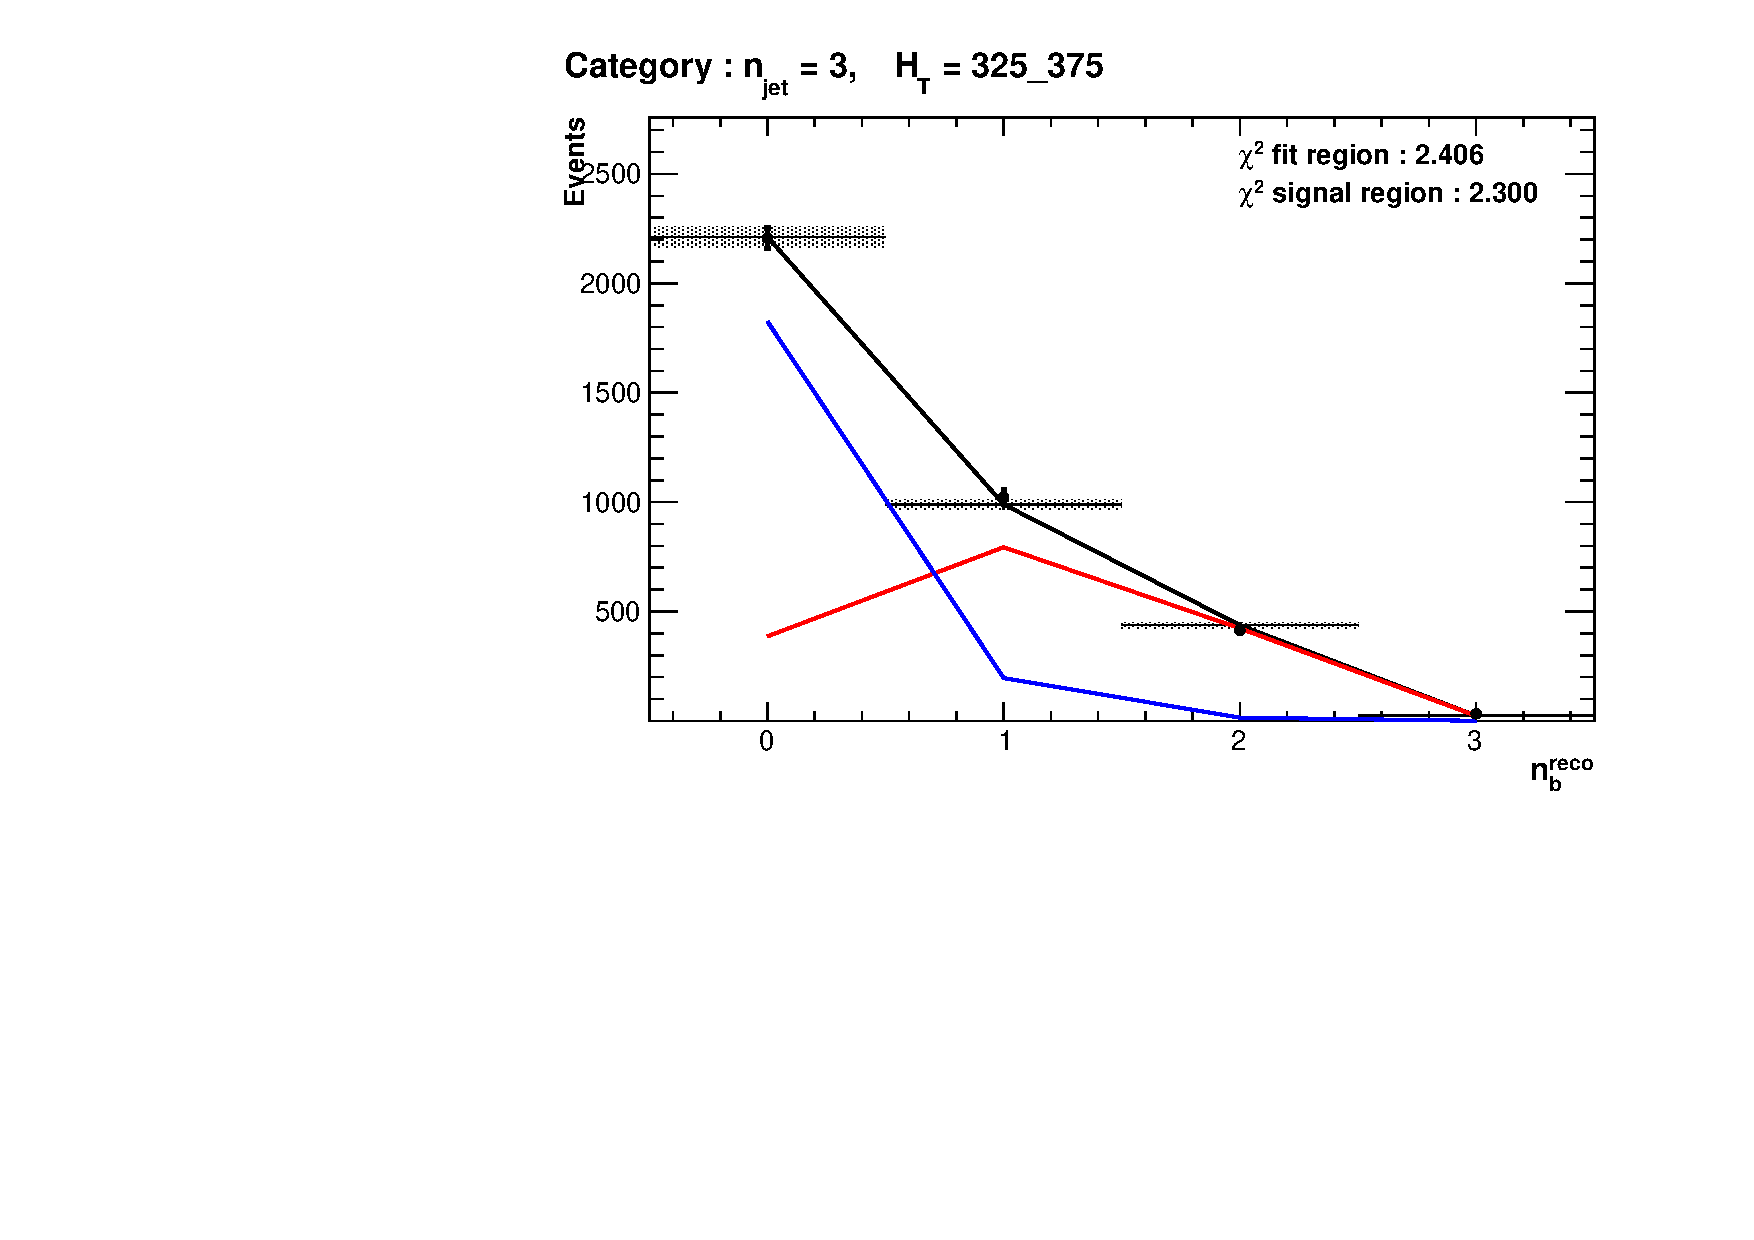
\includegraphics[width = 1.0\linewidth]{plots/ThesisPlots/Final_Fit_To_Data_Normal_Medium_HTBin_OneMuon_325_375_jet_mult_3.pdf}
\centering (b) $n_{jet} =$  3 , 325 $<$ \theht $<$ 375 
\end{minipage}
\quad
\begin{minipage}[b]{0.51\linewidth}
\centering
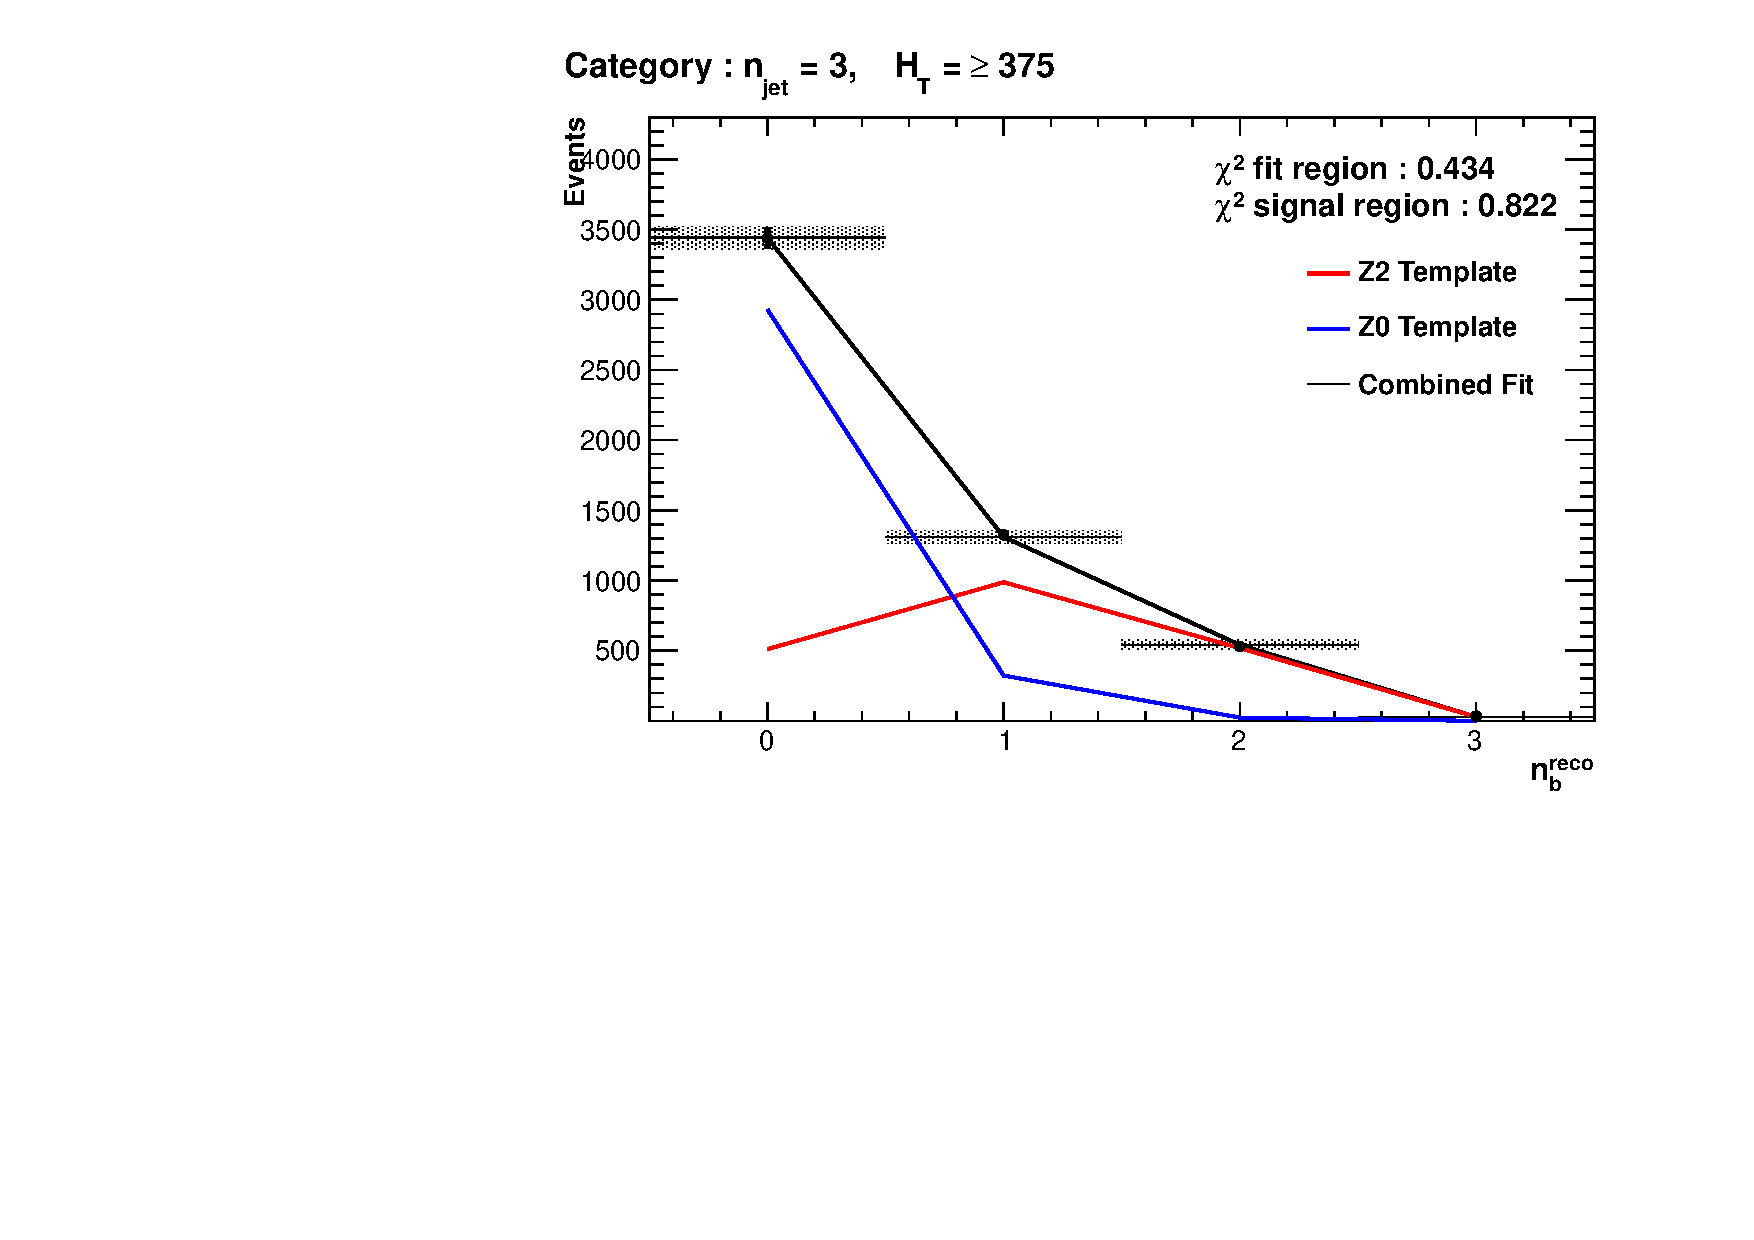
\includegraphics[width = 1.0\linewidth]{plots/ThesisPlots/Final_Fit_To_Data_Normal_Medium_HTBin_OneMuon_Template_375_jet_mult_3.pdf}
\centering (c) $n_{jet} =$ 3 , \theht $>$ 375 
\end{minipage}
\caption[The results of fitting the Z = 0 and Z = 2 templates to the $n_{b}^{reco}$ = 0, 1, 2 bins taken directly from data, for the $n_{jet} = 3$ category and medium \ac{CSV} working point.]{The results of fitting the Z = 0 and Z = 2 templates to the $n_{b}^{reco}$ = 0, 1, 2 bins taken from data, for the $n_{jet} = 3$ category and medium \ac{CSV} working point. The blue template represents Z = 0, while the red template represents Z = 2. The $\chi^{2}$ parameter displayed represents the goodness of fit to the low $n_{b}^{reco}$ (0-2) control region.}
\label{app:template_data_loose_njet5}
\end{figure}
\FloatBarrier

Template fits for the three \theht bins, in the $n_{jet} = 4$,  medium \ac{CSV} working point:

\begin{figure}[ht]
\centering
\begin{minipage}[b]{0.51 \linewidth}
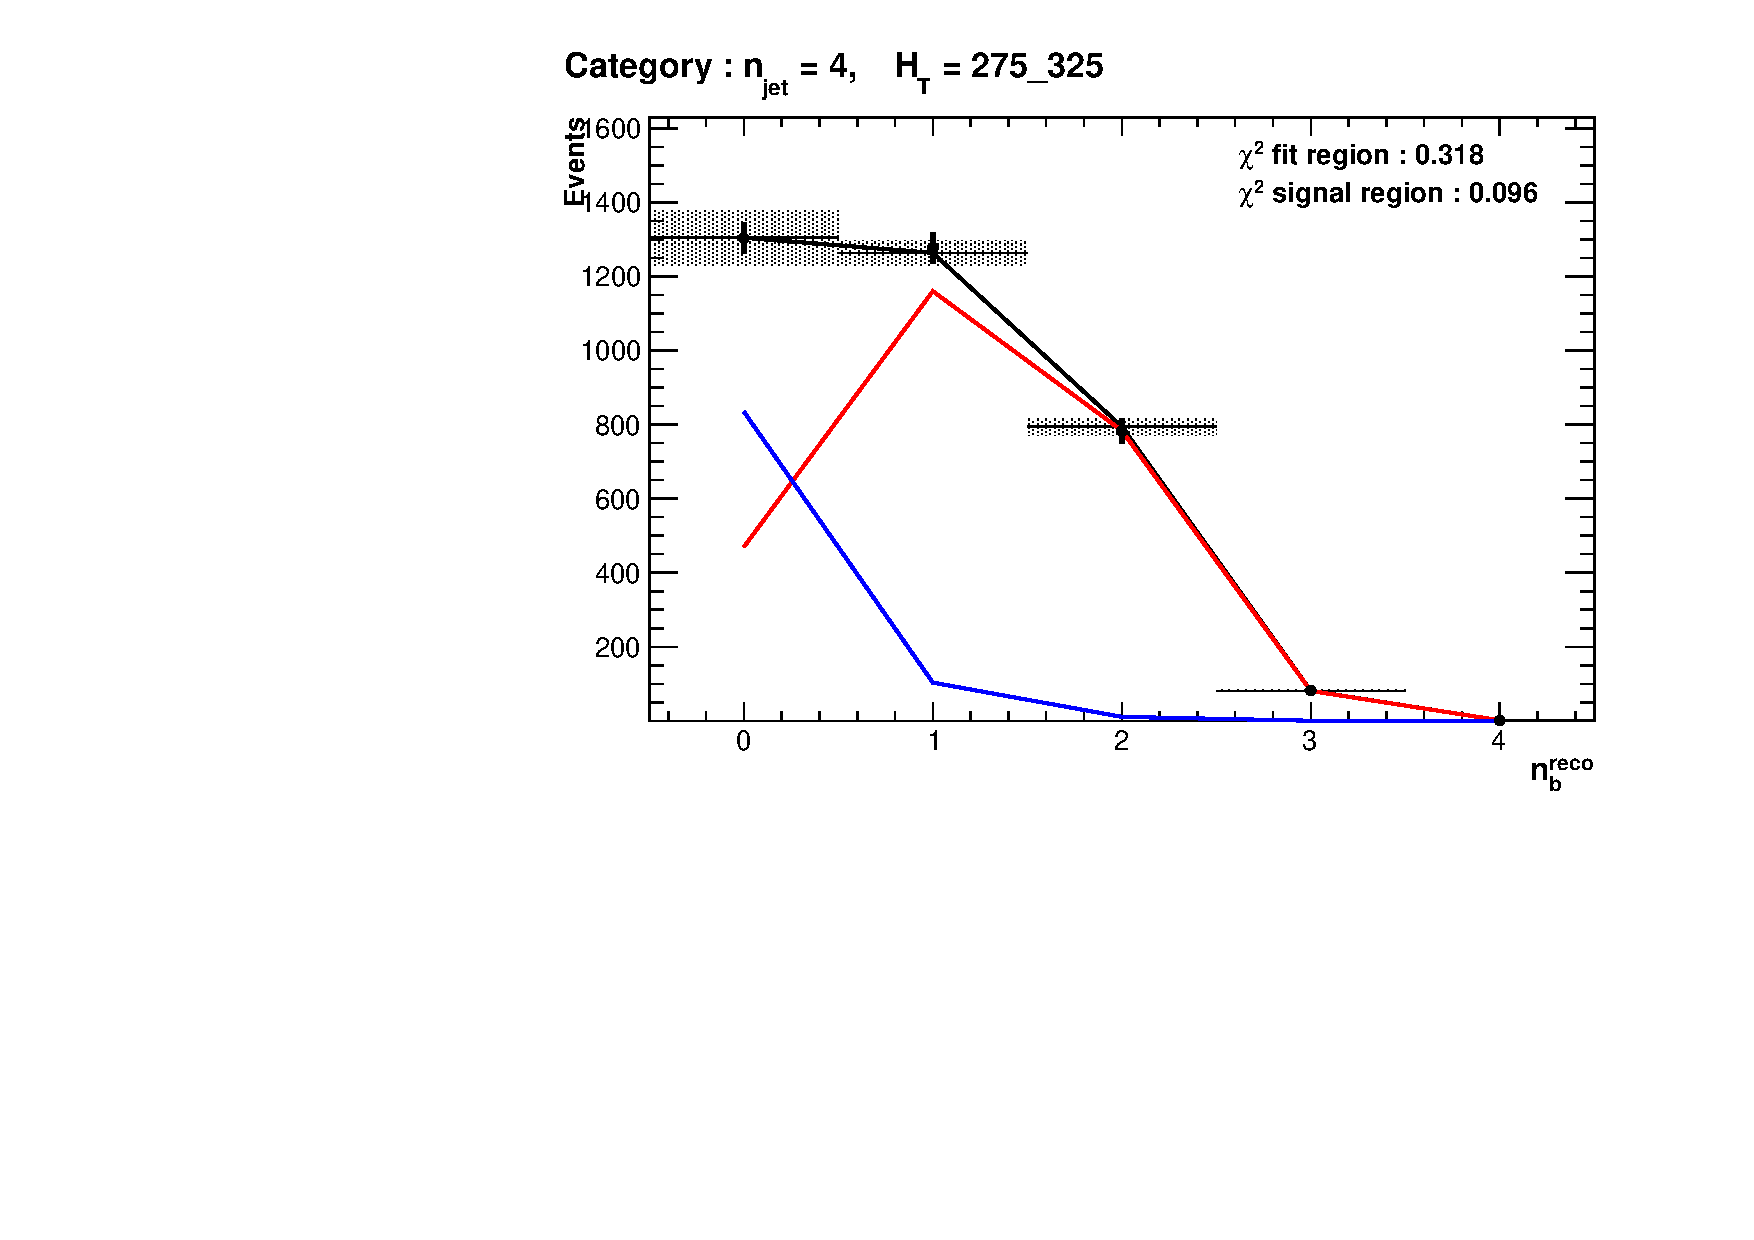
\includegraphics[width = 1.0\linewidth]{plots/ThesisPlots/Final_Fit_To_Data_Normal_Medium_HTBin_OneMuon_275_325_jet_mult_4.pdf}
\centering (a) $n_{jet} =$  4 , 275 $<$ \theht $<$ 325
\end{minipage}
\quad
\begin{minipage}[b]{0.51\linewidth}
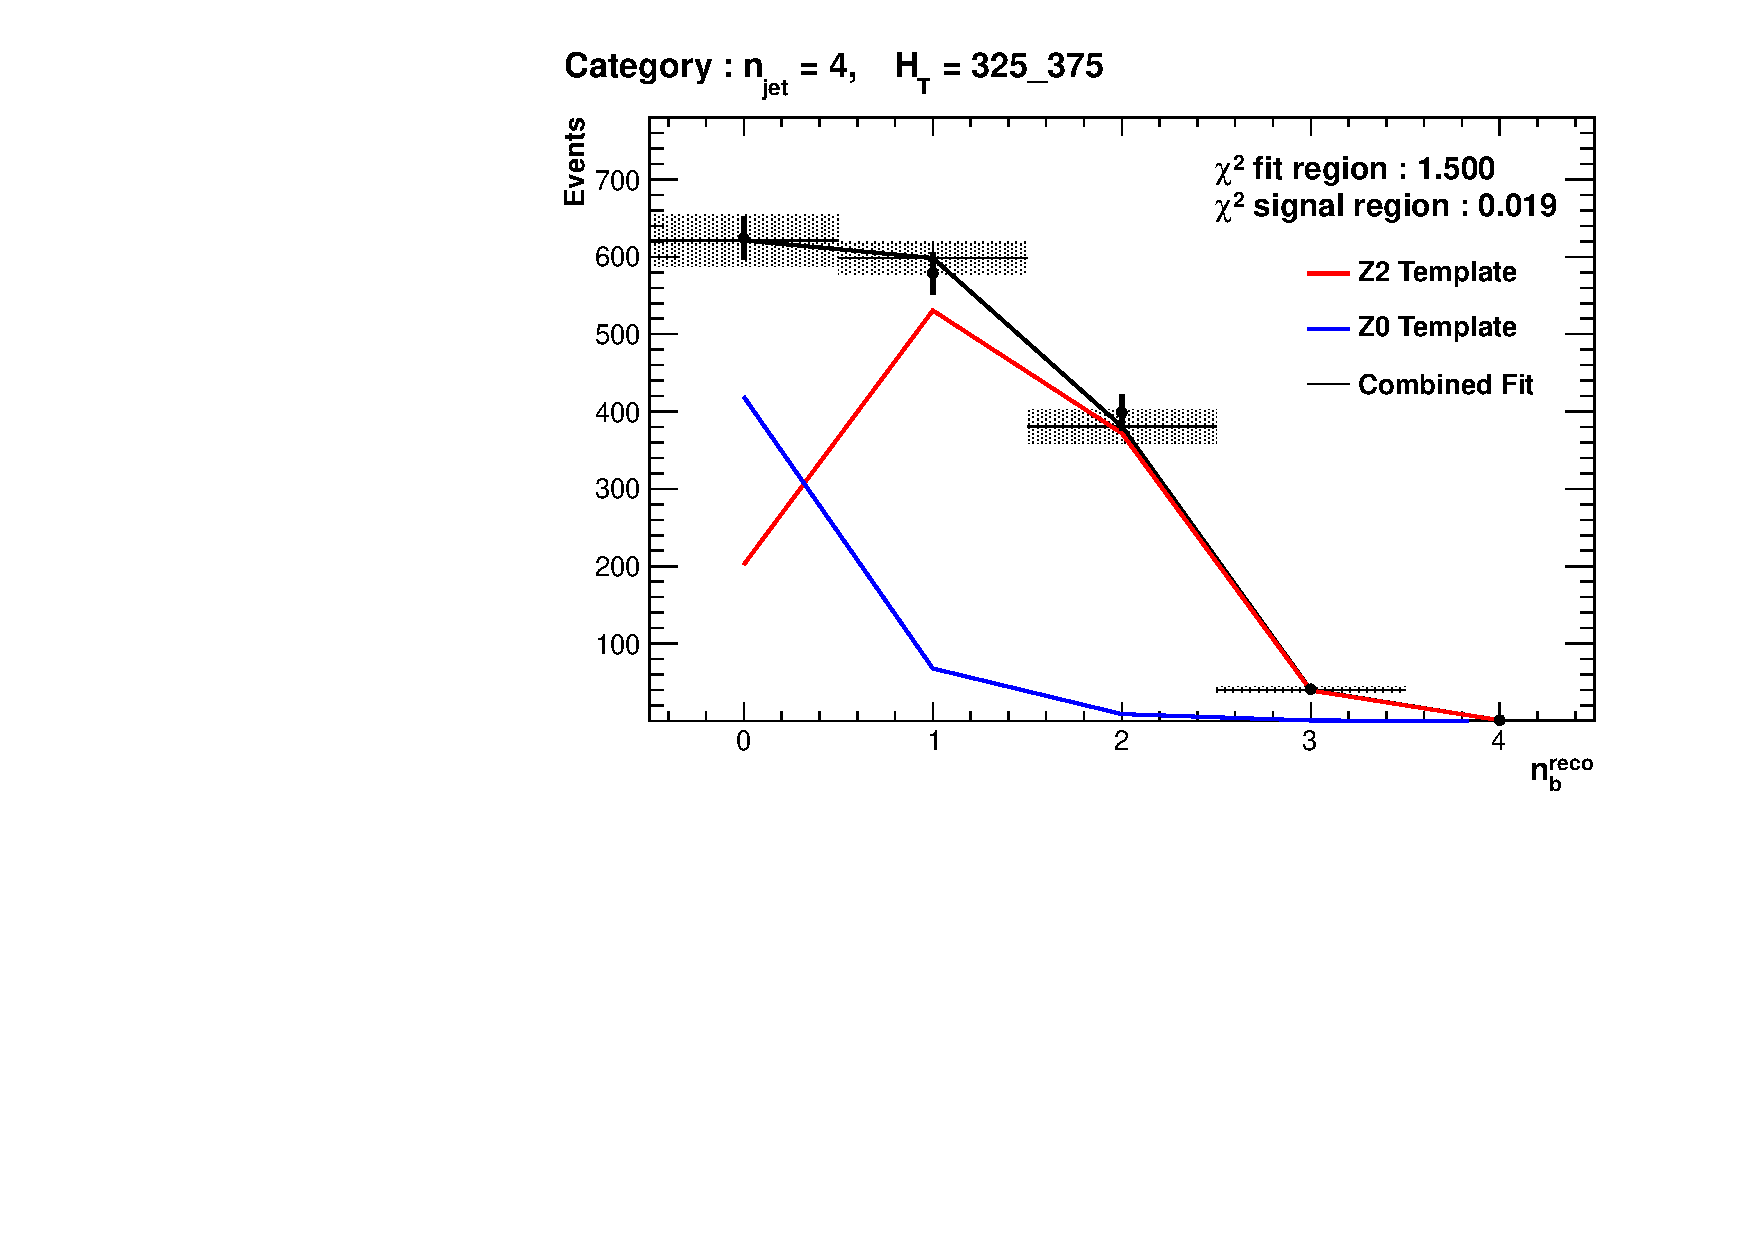
\includegraphics[width = 1.0\linewidth]{plots/ThesisPlots/Final_Fit_To_Data_Normal_Medium_HTBin_OneMuon_325_375_jet_mult_4.pdf}
\centering (b) $n_{jet} =$ 4 , 325 $<$ \theht $<$ 375 
\end{minipage}
\quad
\begin{minipage}[b]{0.51\linewidth}
\centering
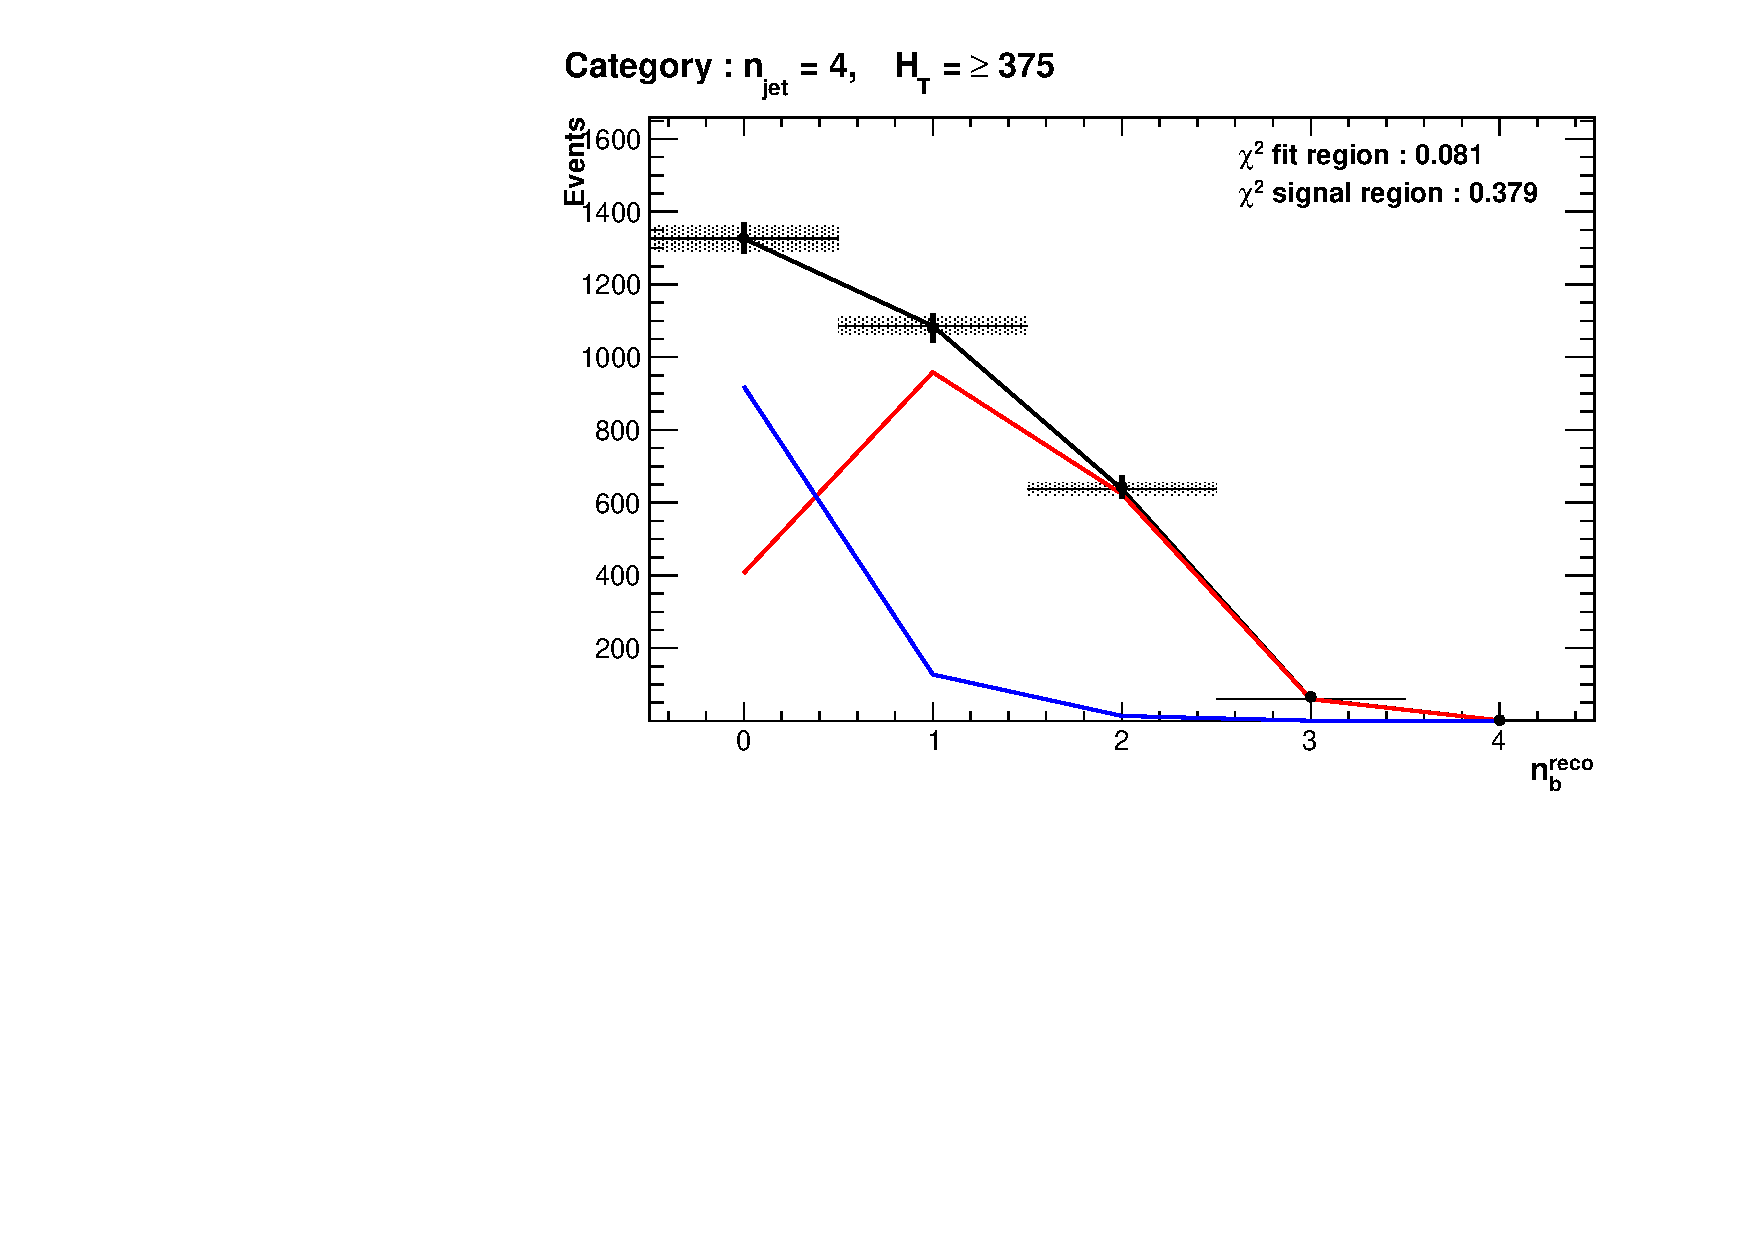
\includegraphics[width = 1.0\linewidth]{plots/ThesisPlots/Final_Fit_To_Data_Normal_Medium_HTBin_OneMuon_Template_375_jet_mult_4.pdf}
\centering (c) $n_{jet} =$ 4 , \theht $>$ 375 
\end{minipage}
\caption[The results of fitting the Z = 0 and Z = 2 templates to the $n_{b}^{reco}$ = 0, 1, 2 bins taken directly from data, for the $n_{jet} = 4$ category and medium \ac{CSV} working point.]{The results of fitting the Z = 0 and Z = 2 templates to the $n_{b}^{reco}$ = 0, 1, 2 bins taken from data, for the $n_{jet} = 4$ category and medium \ac{CSV} working point. The blue template represents Z = 0, while the red template represents Z = 2. The $\chi^{2}$ parameter displayed represents the goodness of fit to the low $ n_{b}^{reco}$ (0-2) control region.}
\label{app:template_data_tight_njet5}
\end{figure}

\section{Templates Fits in Data Signal Region}
\label{app:templatedata_signal}

Template fits for the three \ac{CSV} working points, in the $n_{jet}$ = 3, \theht $>$ 375 category :

\begin{figure}[ht]
\footnotesize
\centering
\begin{minipage}[b]{0.51 \linewidth}
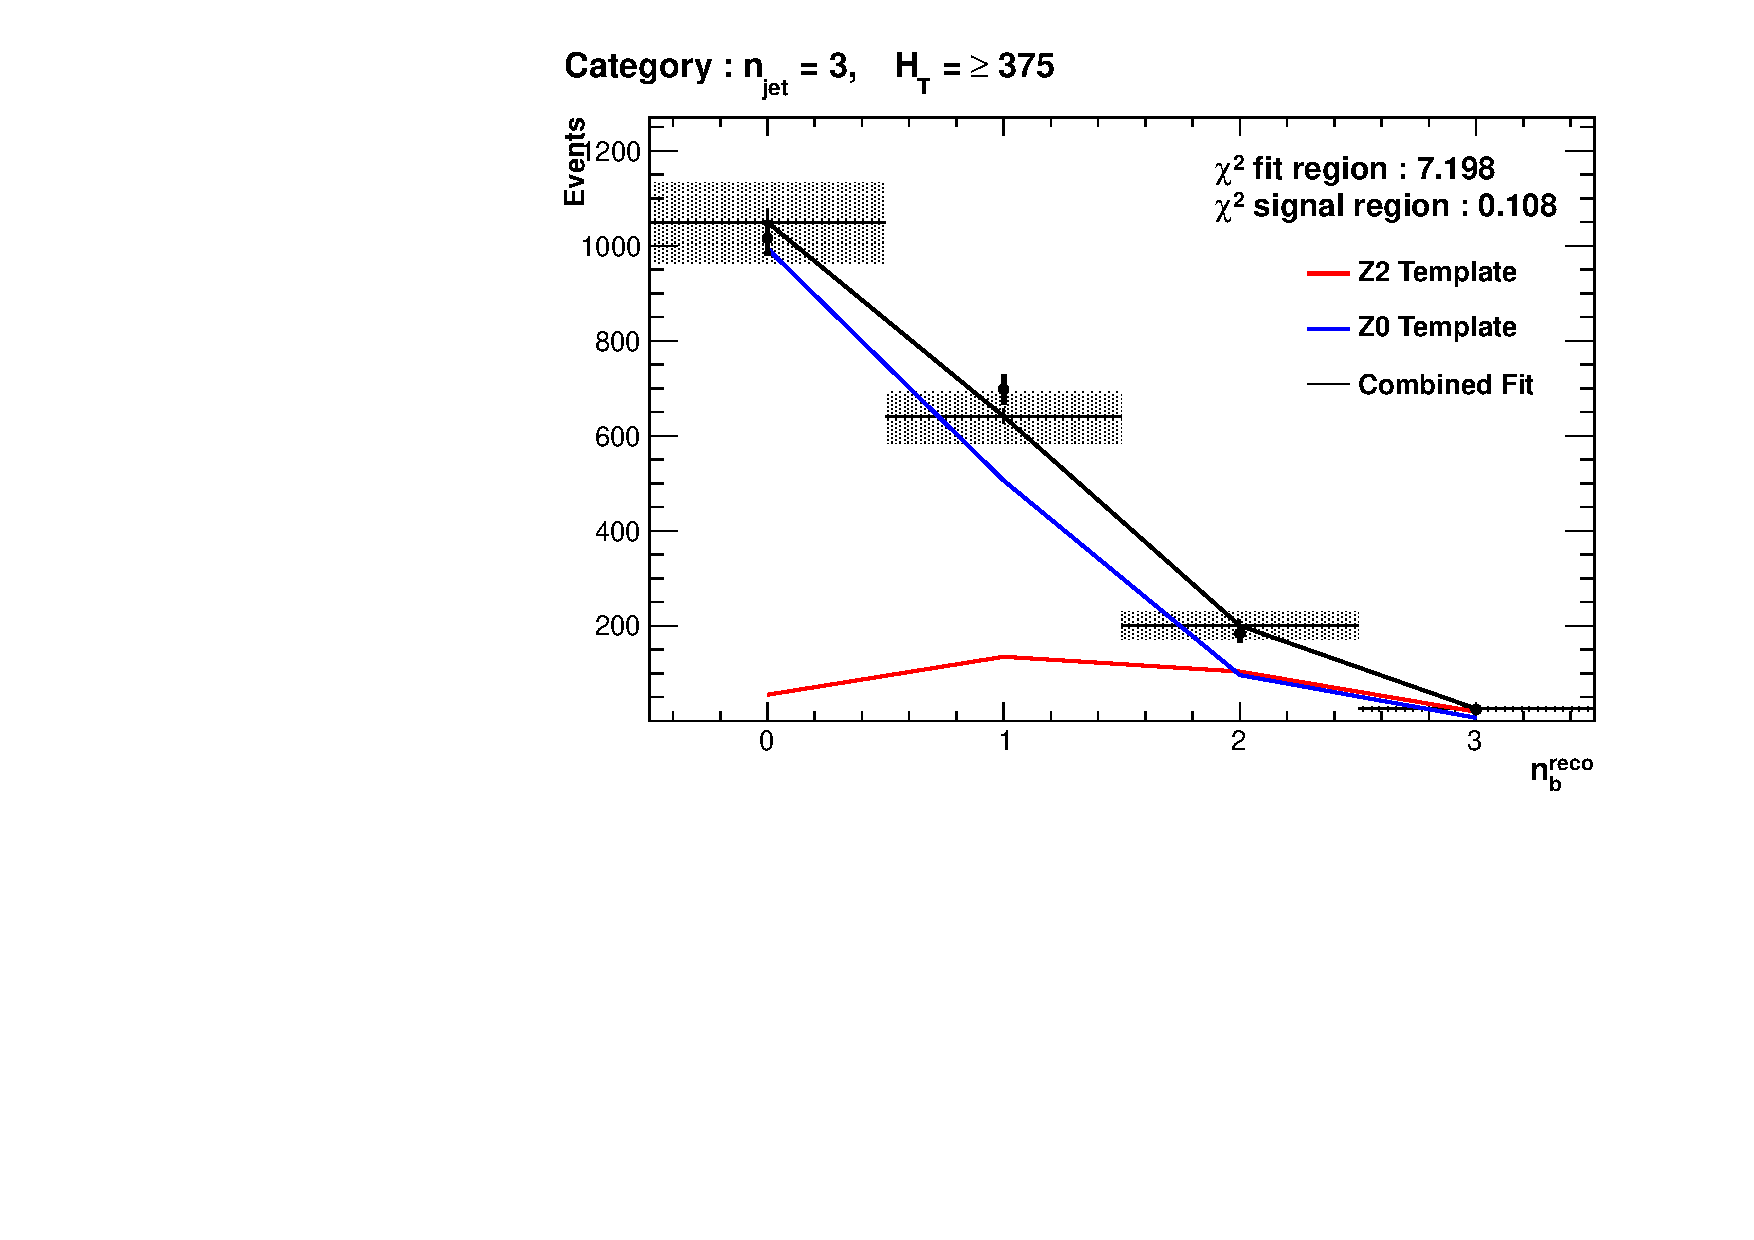
\includegraphics[width = 1.0\linewidth]{plots/TemplatesSignal/Final_Fit_To_Data_Normal_Loose_HTBin_Template_375_jet_mult_3.pdf}
\centering (a) Loose working point : $n_{jet}=$  3 , \theht $>$ 375
\end{minipage}
\quad
\begin{minipage}[b]{0.51\linewidth}
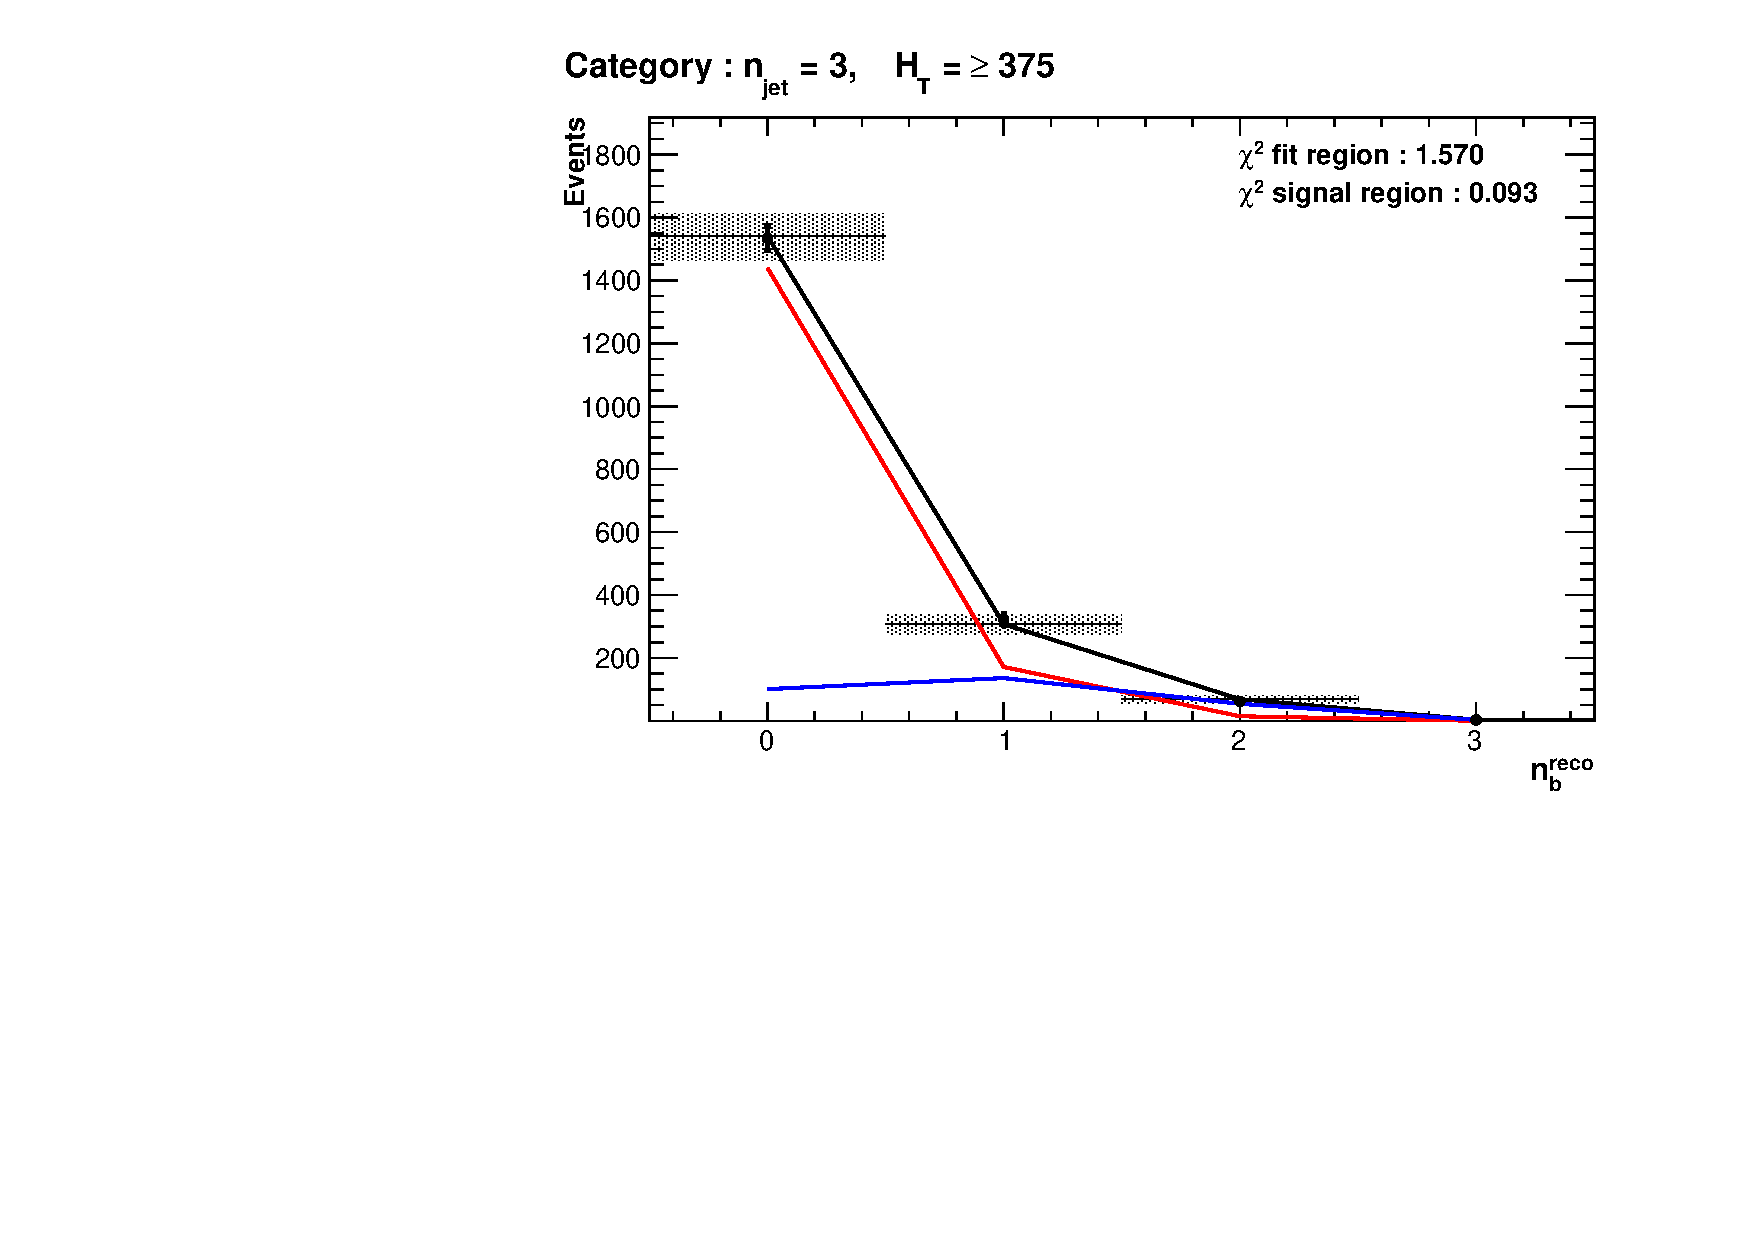
\includegraphics[width = 1.0\linewidth]{plots/TemplatesSignal/Final_Fit_To_Data_Normal_Medium_HTBin_Template_375_jet_mult_3.pdf}
\centering (b) Medium working point : $n_{jet}$ = 3 , \theht $>$ 375 
\end{minipage}
\quad
\begin{minipage}[b]{0.51\linewidth}
\centering
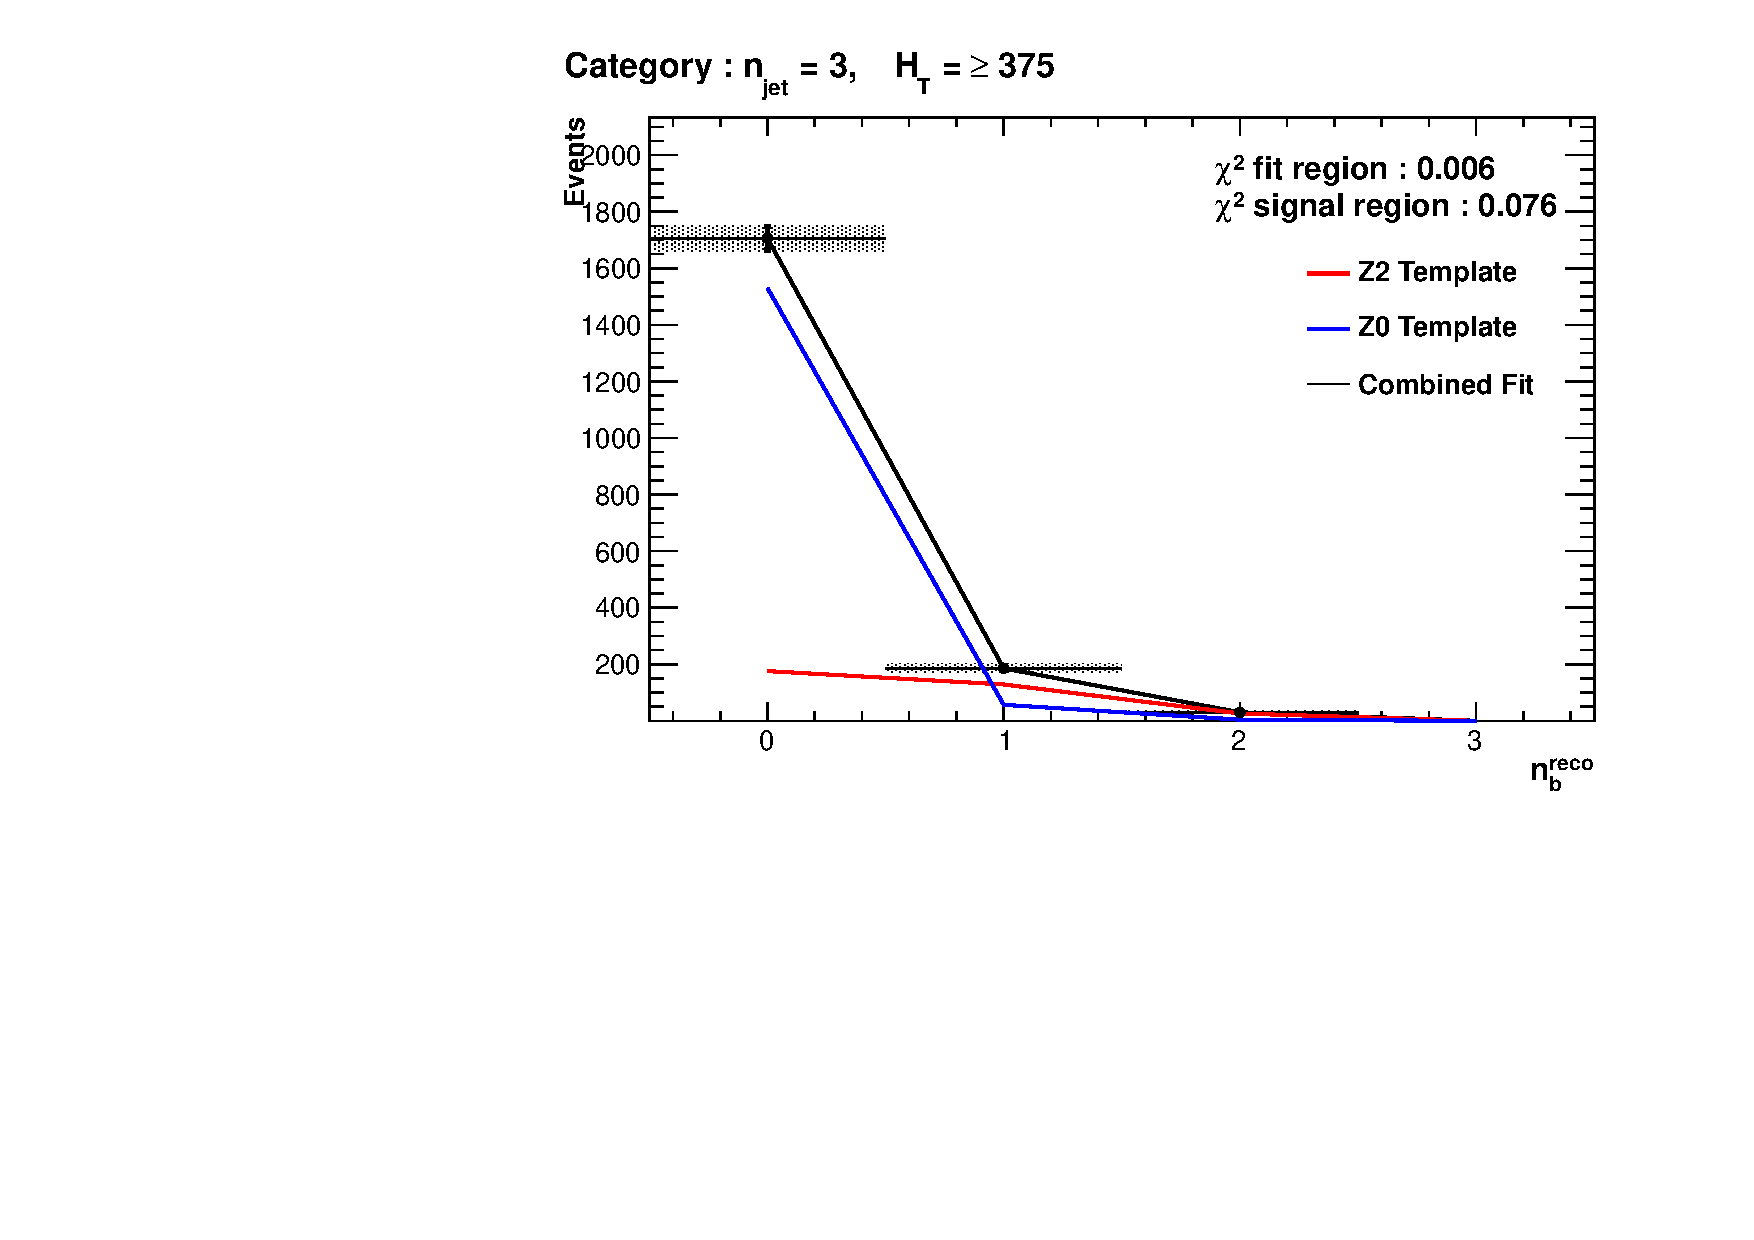
\includegraphics[width = 1.0\linewidth]{plots/TemplatesSignal/Final_Fit_To_Data_Normal_Tight_HTBin_Template_375_jet_mult_3.pdf}
\centering (c) Tight working point :  $n_{jet} =$ 3 , \theht $>$ 375 
\end{minipage}
\caption[The results of fitting the Z = 0 and Z = 2 templates to the $n_{b}^{reco}$ = 0, 1, 2 bins taken from data, in the $n_{jet} = 3$ and \theht $>$ 375 category for all \ac{CSV} working points.]{The results of fitting the Z = 0 and Z = 2 templates to the $n_{b}^{reco}$ = 0, 1, 2 bins taken from data, in the $n_{jet} =3$ and \theht $>$ 375 category for all \ac{CSV} working points. The blue template represents Z = 0, while the red template represents Z = 2. The $\chi^{2}$ parameter displayed represents the goodness of fit to the low$ n_{b}^{reco}$ (0-2) control region.}
\label{app:template_data_signal_njet3}
\end{figure}

Template fits for the three \ac{CSV} working points, in the $n_{jet}$ = 4, \theht $>$ 375 category :

\begin{figure}[ht]
\footnotesize
\centering
\begin{minipage}[b]{0.51 \linewidth}
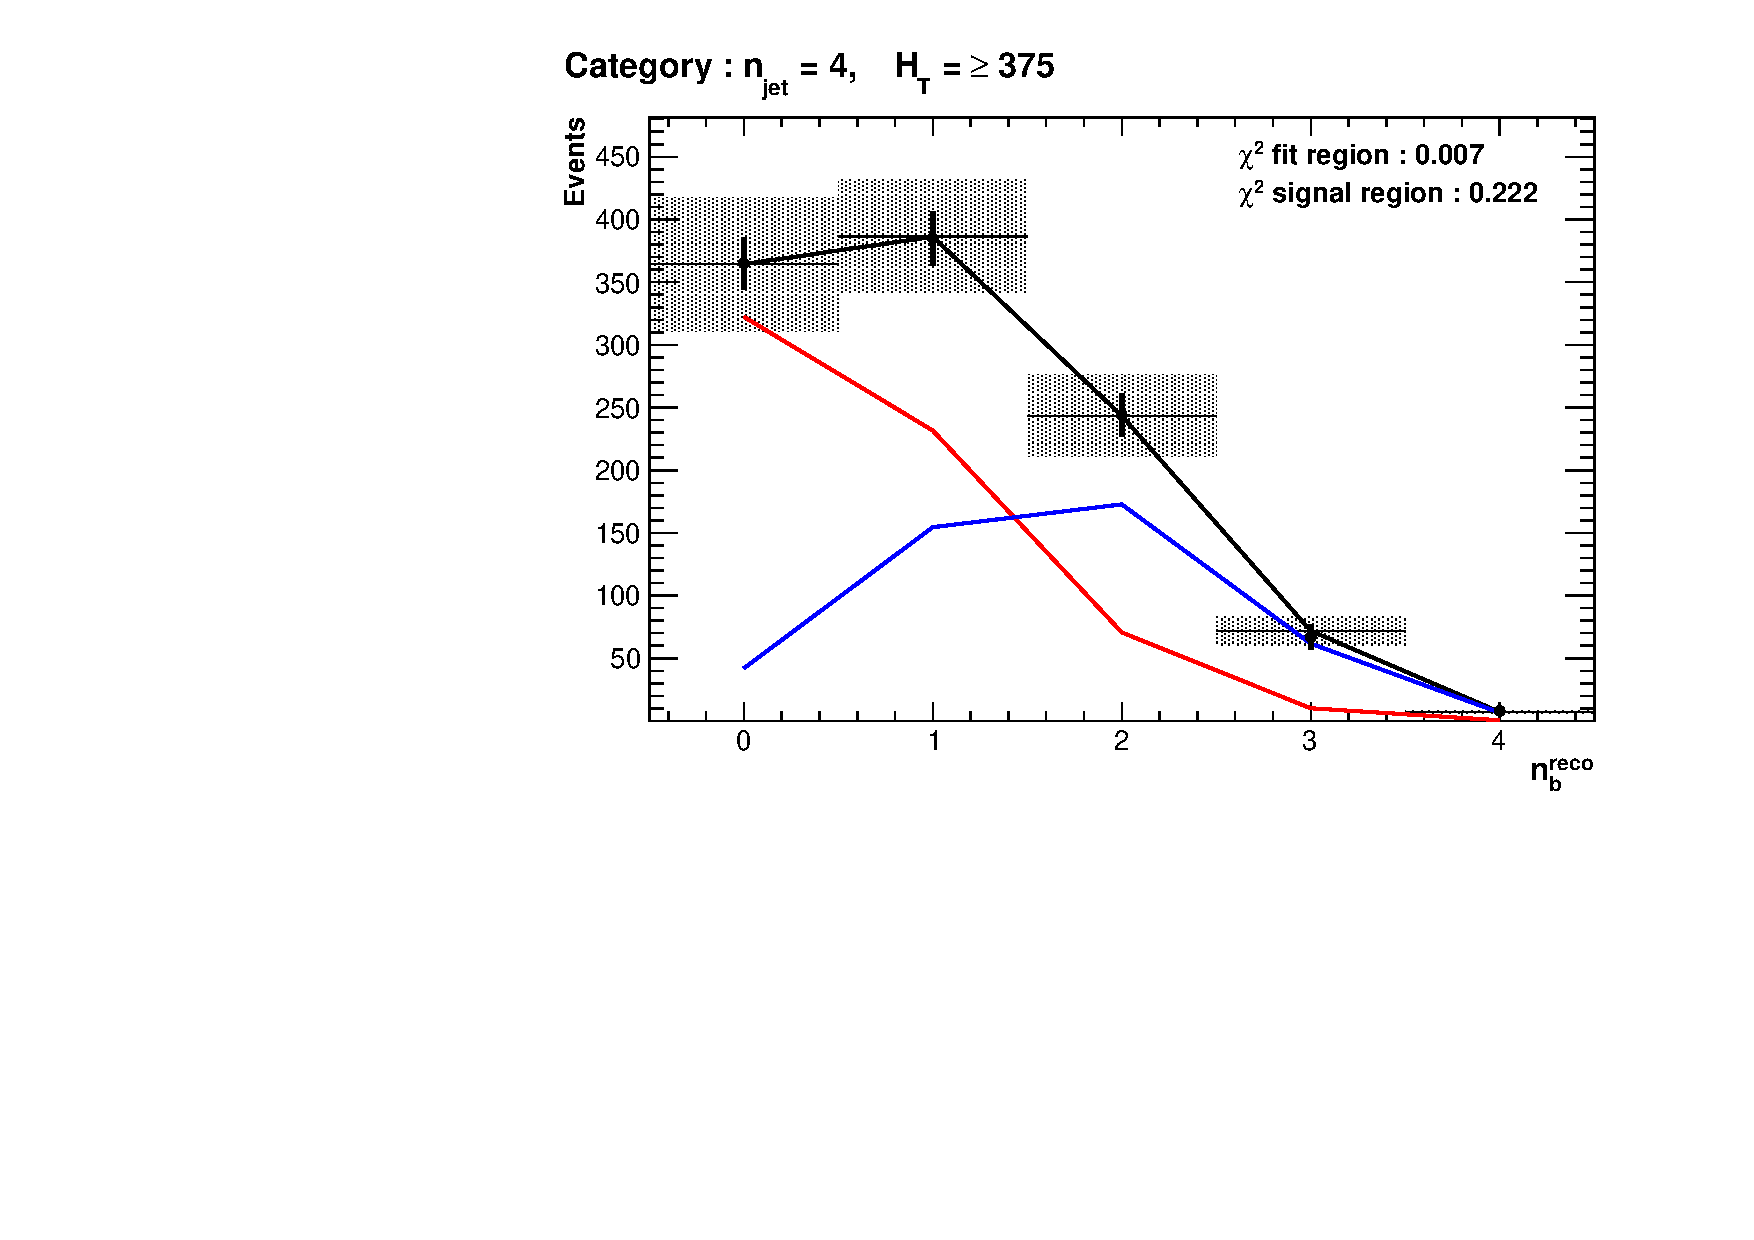
\includegraphics[width = 1.0\linewidth]{plots/TemplatesSignal/Final_Fit_To_Data_Normal_Loose_HTBin_Template_375_jet_mult_4.pdf}
\centering (a) Loose working point : $n_{jet}=$  4 , \theht $>$ 375
\end{minipage}
\quad
\begin{minipage}[b]{0.51\linewidth}
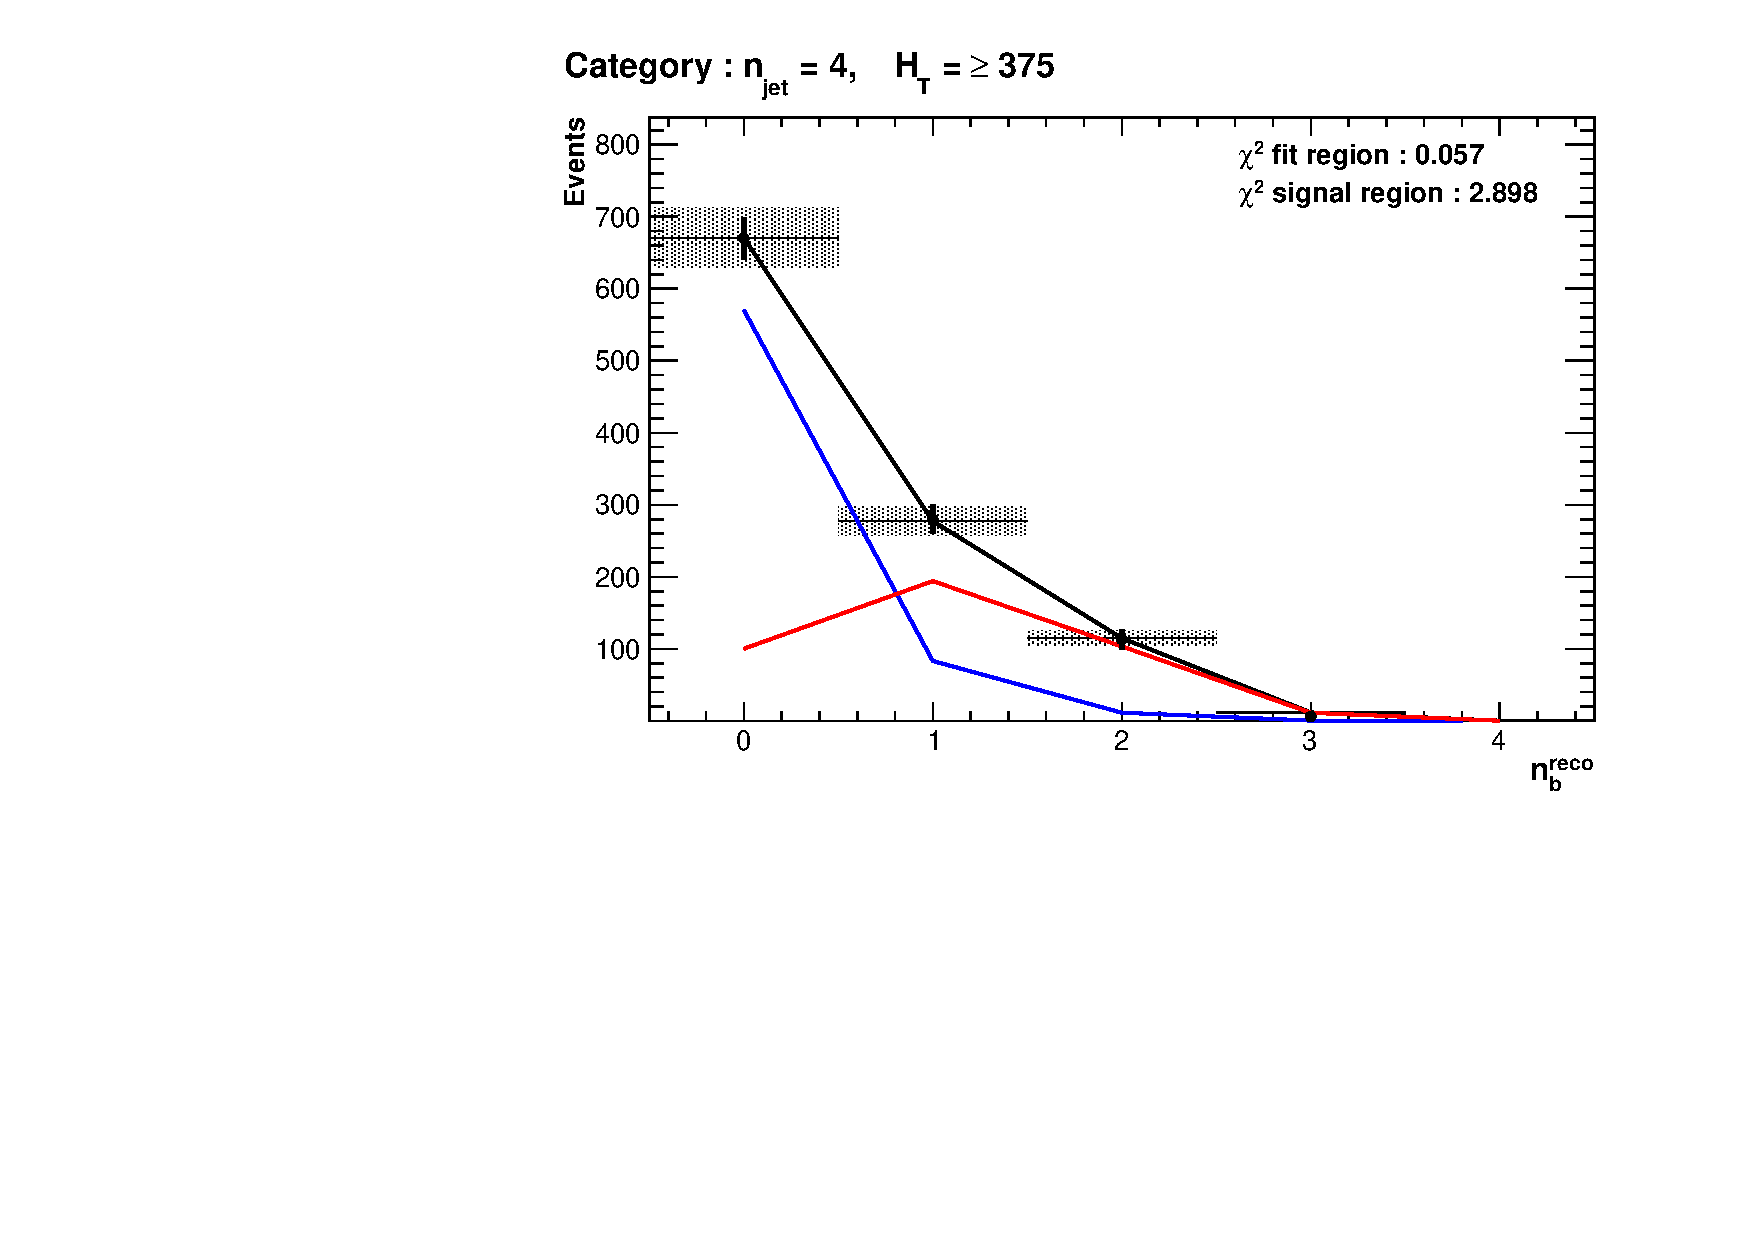
\includegraphics[width = 1.0\linewidth]{plots/TemplatesSignal/Final_Fit_To_Data_Normal_Medium_HTBin_Template_375_jet_mult_4.pdf}
\centering (b) Medium working point : $n_{jet}$ = 4 , \theht $>$ 375 
\end{minipage}
\quad
\begin{minipage}[b]{0.51\linewidth}
\centering
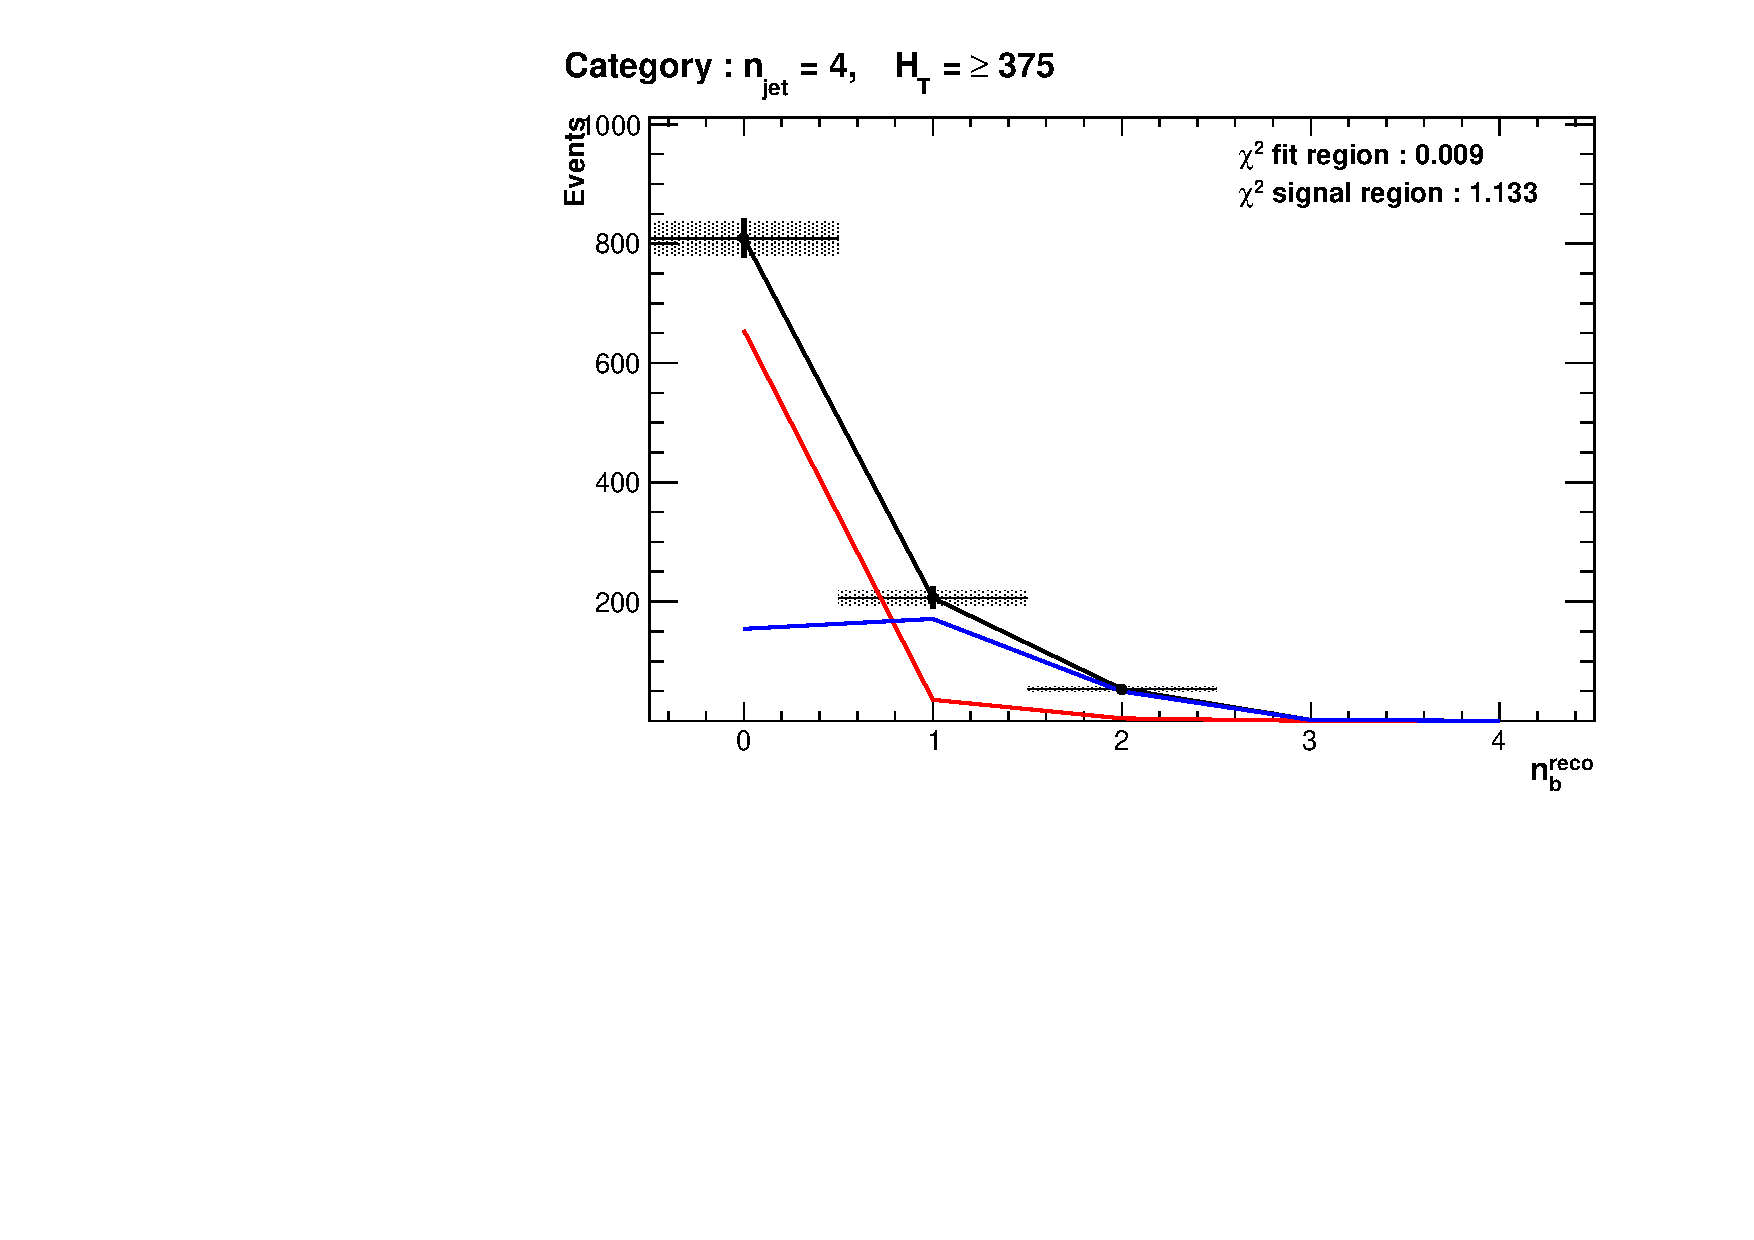
\includegraphics[width = 1.0\linewidth]{plots/TemplatesSignal/Final_Fit_To_Data_Normal_Tight_HTBin_Template_375_jet_mult_4.pdf}
\centering (c) Tight working point :  $n_{jet} =$ 4 , \theht $>$ 375 
\end{minipage}
\caption[The results of fitting the Z = 0 and Z = 2 templates to the $n_{b}^{reco}$ = 0, 1, 2 bins taken from data, in the $n_{jet} = 4$ and \theht $>$ 375 category for all \ac{CSV} working points.]{The results of fitting the Z = 0 and Z = 2 templates to the $n_{b}^{reco}$ = 0, 1, 2 bins taken from data, in the $n_{jet} =4$ and \theht $>$ 375 category for all \ac{CSV} working points. The blue template represents Z = 0, while the red template represents Z = 2. The $\chi^{2}$ parameter displayed represents the goodness of fit to the low$ n_{b}^{reco}$ (0-2) control region.}
\label{app:template_data_signal_njet3}
\end{figure}
